%%%%%%%%%%%%%%%%%%%%%%%%%%%%%%%
%========================================%
%=P=H=Y=S=I=C=S===C=O=M=P=E=N=D=I=U=M=%
%=H=H===================================%
%=Y===Y==================================%
%=S======S===============================%
%=I========I==============================%
%=C=========C============================%
%=S===========S==========================%
%========================================%
%=C===============C======================%
%=O=================O====================%
%=M===================M=================%
%=P======================P===============%
%=E========================E=============%
%=N==========================N===========%
%=D=============================D========%
%=I================================I======%
%=U=================================U===%
%=M===================================M=%
%========================================%
%%%%%%%%%%%%%%%%%%%%%%%%%%%%%%%

\documentclass{article}

\usepackage{braket}
\usepackage{bigints}
\usepackage{hyperref}
\usepackage{array}
\usepackage{graphicx}
\usepackage{enumitem}
\usepackage{mathtools}
\usepackage{esint}
\usepackage{amsfonts}
\usepackage{amsmath}
\usepackage{amsbsy}
\usepackage[margin=1in]{geometry}

\linespread{2.5}
\setlength\parindent{1cm}


%%%%%%%%%%
%% MACROS %%
%%%%%%%%%%

\newcommand{\angst}{\text{\normalfont\AA}}

\newcommand*{\vv}[1]{\vec{\mkern0mu#1}}

\newcommand{\BigP}[1]{\Big( #1 \Big)}

\newcommand{\Mtx}[1]{\textrm{\textbf{\textsf{#1}}}}

\newcommand{\Table}[1]{\center \begin{tabular}{|c|c|} #1 \end{tabular} \flushleft}

\newcommand{\MiniPg}[2]{\begin{minipage}{#1\textwidth} \vspace{3mm} #2 \vspace{3mm} \end{minipage}}

\newcommand{\GraphicWHN}[3]{\center \includegraphics[width=#1\linewidth, height=#2\linewidth]{images/#3}  \flushleft}

\newcommand\SmallMatrix[1]{
\renewcommand\arraystretch{0.44}
\renewcommand \arraycolsep{3pt}
  \small  \begin{pmatrix}#1\end{pmatrix} \large}
  
\newcommand\MPalign[1]{
\centering
\renewcommand\arraystretch{1}
  $\begin{array}{r@{{}\mathrel{}{}}l}
    #1
  \end{array}$
}

%%%%%%%%%%%%%%%%%
%%% WHATS UP DOC? %%%
%%%%%%%%%%%%%%%%%

\begin{document}

\title{Que's Compendium of Memorization and Reference Items for the Hard Working Physicist}
\author{Ethan Que Williams}
\maketitle

This list of physics knowledge bits was originally intended to be a study guide for the physics GRE. As such, the sections are organized in the order of study topics listed by good ol' ETS.

%\large

\tableofcontents


\section{Good numbers to know}

\Table{
\hline

Mass of proton & $1.67 \times 10^{-27}$ kg

\\ \hline

Diameter of proton & about a femtometer $(10^{-15})$
 
\\ \hline

Diameter of an atom & about 0.1 nanometers = 1 \angst

\\ \hline

Mass of electron & $9.1 \times 10^{-31}$ kg
 
\\ \hline

Elementary charge & $1.6 \times 10^{-19}$ C

\\ \hline

Mass of the Earth & $6 \times 10^{24}$ kg

\\ \hline

Radius of the Earth & $6 \times 10^6$ m

\\ \hline

Mass of the Sun & $2 \times 10^{30}$ kg

\\ \hline

Radius of the Sun & 10,000 km = $7 \times 10^8 $ m

\\ \hline

The astronomical unit & 150 million km = $1.5 \times 10^{11} $ m

\\ \hline

Density of water & 1000 kg/m$^3$

 \\ \hline

}

%===========================================%

\Table{
\hline
\MiniPg{.2}{
Wavelength frequency ranges of visible light. 
}
&
\MiniPg{.6}{
\GraphicWHN{.6}{.4}{color_wavelength_frequency.png}

\tiny \url{http://reikiservices.cfsites.org/files/color_wavelength_frequency.png}
}
 \\ \hline

}

%===========================================%

\GraphicWHN{.9}{.5}{EM_Spectrum.png}
\center
\tiny \url{https://xkcd.com/273/} \large
\flushleft

%%%%%%%%%%%%%%%%%%%%%%%%%%%%%%%%%
%===========================================%
%%%%%%%%%%%%%%%%%%%%%%%%%%%%%%%%%



\section{Math}

\Table{
\hline

\MiniPg{.3}{
Normal Gaussian Distribution
}
&

\MiniPg{.7}{
\center

$f(x) = \dfrac{1}{\sqrt{2 \sigma^2 \pi}} e^{- \frac{(x- \mu)^2}{2 \sigma^2}}$,

where $\mu$ is expectation, $\sigma$ is standard deviation, $\sigma^2$ is variance.

}

\\ \hline

Empirical Rule

&

\MiniPg{.7}{

\GraphicWHN{1}{.57}{Empirical_Rule.PNG}.
\tiny Stolen without permission from the internet.
}

\\ \hline
}


%===========================================%


\subsection{Trigonometry}
\center

\GraphicWHN{.6}{.6}{UnitCircle.png}
\center \tiny \url{https://en.wikipedia.org/wiki/Unit_circle} \large

\Table{
\hline
\MiniPg{.3}{\center
$\dfrac{\sqrt{2}}{2}$
}
&
\MiniPg{.7}{\center
$\dfrac{\sqrt{2}}{2} \approx \dfrac{1.4}{2} = 0.7$
}
\\ \hline

$\dfrac{\sqrt{3}}{2}$

&

$\dfrac{\sqrt{3}}{2} \approx \dfrac{1.7}{2} = .85$

\\ \hline
}

%%%%

\Table{
\hline

First three pythagorean triples

&
\MiniPg{.6}{\center
$(3, 4, 5), \ \ \ (5, 12, 13), \ \ \ (8, 15, 17)$
}

\\ \hline
}

%%%%

\Table{
\hline

$\sin(\theta \pm \phi) = $ 
&
\MiniPg{.7}{ \center
$\sin(\theta)\cos(\phi) \pm \cos(\theta) \sin(\phi)$
}

\\ \hline

$\cos(\theta \pm \phi) = $ & $ \cos(\theta) \cos(\phi) \mp \sin(\theta) \sin(\phi)$

\\ \hline

$\cos(\theta) \cos(\phi) = $ & $  \dfrac{1}{2}[\cos(\theta + \phi) + \cos(\theta - \phi)]$

\\ \hline

$\sin(\theta) \sin(\phi) = $ & $  \dfrac{1}{2}[\cos(\theta - \phi) - \cos(\theta + \phi)]$

\\ \hline

$\sin(\theta) \cos(\phi) = $ & $ \dfrac{1}{2}[\sin(\theta + \phi) + \sin(\theta - \phi)]$

\\ \hline

}

%%%%

\Table{
\hline

$\sin(\theta) + \sin(\phi) = $ 

& 

\MiniPg{.7}{
\center 
$2 \sin\Big(\dfrac{\theta + \phi}{2} \Big) \, \cos \Big(\dfrac{\theta - \phi}{2} \Big) $
}

\\ \hline

$\sin(\theta) - \sin(\phi) = $ & $2 \sin\Big(\dfrac{\theta - \phi}{2} \Big) \, \cos \Big(\dfrac{\theta + \phi}{2} \Big) $

\\ \hline

$\cos(\theta) + \cos(\phi) = $ & $2 \cos\Big(\dfrac{\theta - \phi}{2} \Big) \, \cos \Big(\dfrac{\theta + \phi}{2} \Big) $

\\ \hline

$\cos(\theta) - \cos(\phi) = $ & $- 2 \sin\Big(\dfrac{\theta - \phi}{2} \Big) \, \sin \Big(\dfrac{\theta + \phi}{2} \Big) $

\\ \hline
}


\Table{
\hline
$\cos^2(\theta) = $ & 
\MiniPg{.7}{\center
$\dfrac{1}{2}[1 + \cos(2\theta)]$
}

\\ \hline

$\sin^2 (\theta) = $ & $ \dfrac{1}{2}[1-\cos(2 \theta)]$

\\ \hline

$\cos^2(\theta) + \sin^2(\theta) = $ & $ 1$

\\ \hline

$e^{i \theta} = $ & $ \cos \theta + i \sin \theta$

\\ \hline

$\cos \theta = $ (Euler's) & $ \dfrac{1}{2}(e^{i \theta} + e^{-i \theta}) $

\\ \hline

$\sin \theta = $ (Euler's) & $ \dfrac{1}{2i}(e^{i \theta} - e^{-i \theta}) $

\\ \hline
}


%===========================================%


\subsection{Calculus}

\Table{
\hline

\MiniPg{.3}{
The first fundamental theorem of calculus...}
&
\MiniPg{.7}{ ... states that if $f$ is continuous on the
closed interval $[a,b]$ and $F$ is the indefinite integral of $f$ on $[a,b]$ then
$\int^b_a f(x) dx = F(b) - F(a)$.}

\\ \hline

\MiniPg{.3}{
The second fundamental theorem of calculus ... }
&
\MiniPg{.7}{... holds for $f$, a continuous
function on an open interval $l$, and $a$, any point in $l$, and states that if $F$ is defined by the integral (antiderivative) $F(x) = \int^x_a f(x) dt$, then $F'(x) = f(x)$ at each point in $l$, where $F'(x)$ is the derivative of $F(x)$.}

\\ \hline

If $f=f(x,y)$ then $df = $ & $\dfrac{\partial f}{\partial x}dx + \dfrac{\partial f}{\partial y}dy$

\\ \hline
}

\Table{
\hline

Chain rule &
\MiniPg{.6}{

If we have z(y) and y(x), then $\dfrac{dz}{dx} = \dfrac{dz}{dy} \cdot \dfrac{dy}{dx}$

}

\\ \hline
}


%===========================================%


\subsection{Taylor and Maclaurin series}

\Table{
\hline
\MiniPg{.3}{
\center
$f(x) = $

Expand about the point $a$.}
&
\MiniPg{.7}{\center
$ f(a) + f'(a)(x-a) + \dfrac{1}{2!}f''(a)(x-a)^2 +\, \dfrac{1}{3!}f'''(a)(x-a)^3 ...$
}
\\ \hline

$e^x = $ & $1 + x + \dfrac{1}{2!}x^2 + \dfrac{1}{3!}x^3 + ...$

\\ \hline

$(1+x)^n = $ & $ 1 + nx + \dfrac{n(n-1)}{2!}x^2 + ... [|x|<1]$ [binomial series]

\\ \hline

$\cos(x) = $ & $ 1 - \dfrac{1}{2!}x^2 + \dfrac{1}{4!}x^4 + ... $

\\ \hline

$\cosh(x) = $ & $ 1 + \dfrac{1}{2!}x^2 + \dfrac{1}{4!}x^4 + ...$

\\ \hline
}

%%%%

\Table{
\hline

$\sin(x) = $
&
\MiniPg{.7}{
\center

$x - \dfrac{1}{3!}x^3 + \dfrac{1}{5!}x^5 - ...$

Also, for small angles, $\sin \theta \approx \tan \theta$.

} 
 \\ \hline

$\sinh(x) = $ & $x + \dfrac{1}{3!}x^3 + \dfrac{1}{5!}x^5 + ...$

\\ \hline

$\tan(x) = $ & $x + \dfrac{1}{3!}x^3 + \dfrac{1}{15!}x^5 + ... [|x|<\pi / 2]$

\\ \hline

$\tanh(x) = $ & $x - \dfrac{1}{3!}x^3 + \dfrac{1}{15!}x^5 - ... [|x|<\pi / 2]$

\\ \hline

$\ln(1 + x) = $ & $x - \dfrac{1}{2}x^2 +\dfrac{1}{3}x^3 - ... [|x| < 1]$

\\ \hline


}

%===========================================%

\subsection{Vector Calculus}  

\Table{
\hline

Laplacian &

\MiniPg{.5}{\center
 $\nabla^2 T = \vv{\nabla} \cdot (\vv{\nabla}T) = \dfrac{\partial^2T}{\partial x^2} + \dfrac{\partial^2T}{\partial y^2} +\dfrac{\partial^2T}{\partial z^2}$

$\nabla^2\vv{v} = \nabla^2v_x \hat x + \nabla^2v_y \hat y +\nabla^2v_z \hat z$
}

\\ \hline

\MiniPg{.4}{\center
What are the two zero vector derivatives? }
&
\MiniPg{.5}{\center
 $\vv{\nabla} \times(\vv{\nabla}T) = 0 $ 

$\vv{\nabla} \cdot (\vv{\nabla} \times \vv{v}) = 0$
}
\\ \hline

$\vv{\nabla} \times (\vv{\nabla} \times \vv{v} ) $ =  & $\vv{ \nabla}(\vv{\nabla} \cdot \vv{v} ) - \nabla^2 \vv{v} $

\\ \hline

Gradient Theorem: 	&
\MiniPg{.5}{\center
 $ \int_a^b (\vv{\nabla}f) \cdot d\vv{l} = f(b) - f(a) $  
 
  Independent of Path. 
  
  $\oint (\vv{\nabla}f) \cdot d\vv{l} = 0 $
}
\\ \hline

Stoke's Theorem: & $ \int_{surface} (\vv{\nabla} \times \vv{v}) \cdot d\vv{a} = \oint_{path} \vv{v} \cdot d\vv{l} $

\\ \hline

Green's (Divergence) Theorem: & $ \int_{volume}(\vv{\nabla} \cdot \vv{v}) d\tau = \oint_{surface} \vv{v} \cdot d\vv{a}$

\\ \hline

}


%%%%%%%%%%%%%%%%%%%%%%%%%%%%%%%%%%%%%%%%%%%%

\subsection{Matrices}

\Table{
\hline

\MiniPg{.3}{
Typical eigenvalue problem
}
&

\MiniPg{.7}{
\center

\MPalign{
\hat{T} \ket{\alpha} &= \lambda \ket{\alpha} \\
\Mtx{T}\Mtx{a} &= \lambda \Mtx{a} \\
(\Mtx{T} - \lambda \Mtx{I})\Mtx{a} &= \Mtx{0} 
}

\flushleft
By assumption, $\Mtx{a} \neq \Mtx{0}$, so $(\Mtx{T} - \lambda \Mtx{I})$ is singular: $\textrm{det}(\Mtx{T} - \lambda \Mtx{I}) = 0$. This gives an algebraic equation for $\lambda$, which is called the characteristic equation for the matrix; its solutions determine the eigenvalues:

\center
$C_n\lambda^n + C_{n-1}\lambda^{n-1} + ... + C_1 \lambda + C_0 = 0$,

\flushleft
where $n$ is the dimensionality of the vector space. By what's apparently called the `fundamental theorem of algebra', there are $n$ complex roots (the eigenvalues). Well, for an $n\times n$ matrix, there is at least one and at most $n$ distinct eigenvalues. The collection of the eigenvalues of a matrix is called its spectrum. If two or more linearly independent eigenvectors share the same eigenvalue, the spectrum is degenerate. To construct the eigenvectors, plug each $\lambda$ back into $\Mtx{T}\Mtx{a} = \lambda \Mtx{a}$ and solve by one-by-one. \tiny This entry paraphrased and largely quoted from Griffiths, \textit{Introduction to Quantum Mechanics} Appendix 5.

}

\\ \hline
}

%%%%

\Table{
\hline

Diagonalization

&

\MiniPg{.7}{
\center

If the eigenvectors span the space, they can be used as a basis.

$\hat{T} \ket{f_n} = \lambda \ket{f_n}$,

$\Mtx{T} =
\SmallMatrix{
\lambda_1 & 0 & ... & 0 \\
0 & \lambda_2 & ... & 0 \\
\vdots & \vdots & .\vdots. & \vdots \\
0 & 0 & ... & \lambda_n
}$

and the normalized eigenvectors are

$\SmallMatrix{1 \\0 \\ \vdots \\ 0}, \SmallMatrix{0 \\ 1 \\ \vdots \\ 0}, ...,\SmallMatrix{0 \\0 \\ \vdots \\ 1}$.

A matrix that can be brought to diagonal form by a change of basis is said to be diagonalizable. Also note that the trace of a matrix (sum of the diagonal components) is invariant under transformation.

 \tiny This entry paraphrased and largely quoted from Griffiths, \textit{Introduction to Quantum Mechanics} Appendix 5.
}

\\ \hline
}

































\section{Classical Mechanics}
(such as kinematics, Newton’s laws, work and
energy, oscillatory motion, rotational
motion about a fixed axis, dynamics of
systems of particles, central forces and
celestial mechanics, three-dimensional
particle dynamics, Lagrangian and
Hamiltonian formalism, noninertial
reference frames, elementary topics in
fluid dynamics)



\subsection{Kinematics} 
\Table{
\hline

$v(t) = $ & $v(t) = v_0 + at$

\\ \hline

$x(t) = $ & $x(t) = x_0 + vt + \dfrac{1}{2}at^2$

\\ \hline

\MiniPg{.4}{$v(x)$ in uniform acceleration }

&

\MiniPg{.6}{
\center

$KE = KE_0 + W$

$\dfrac{1}{2}mv^2 = \dfrac{1}{2}m v_0^2 +  ma(x-x_0)$

$v(x) = \sqrt{v_0^2 + 2a(x - x_0)}$

}

\\ \hline

}

%%%%

\Table{
\hline

Projectile motion: $v_{xi} = $ & $v_{xi} = v_i\cos\theta_{i}$

\\ \hline

Projectile motion: $v_{yi} = $ & $v_{yi} = v_i\sin\theta_{i}$

\\ \hline

\MiniPg{.3}{
Acceleration (tangential) of a particle on a fixed track, $y(x)$, in a gravitational field
}

&

\MiniPg{.7}{

Position vector for the track: $\vec f(x) = (x, y(x))$.

Tangential vector: $\vec T(x) = \frac{d \vec f}{dx} = (1, \frac{dy}{dx}). $

Tangential acceleration: $a(x) = \vec g \cdot  \dfrac{\vec T}{|\vec T|}. $ 

Supposing $\vec g$ is in the $y$-direction, $\boxed{a(x) = \dfrac{g\,T_y}{|\vec T|}}.$
}
\\ \hline
}


%===========================================%


\subsection{Newton's Laws, implications, common forces} 

\Table{
\hline

Newton's Law I

&

\MiniPg{.7}{
\center

Law of Inertia: Every body persists in its state of being at rest or of moving uniformly straight forward, except insofar as it is compelled to change its state by force impressed. 
}

\\ \hline
}

%%%%

\Table{
\hline

Newton's Law II

&

\MiniPg{.7}{
\center
Force Law: The alteration of motion is ever proportional to the motive force impress'd; and is made in the direction of the right line in which that force is impress'd.

$\bold{F}_{net} = \dfrac{d \bold{p} }{dt} = m\bold{a}$
}

\\ \hline
}

%%%%

\Table{
\hline
Newton's Law III

&

\MiniPg{.7}{
\center
Action-Reaction Law: To every action there is always opposed an equal reaction: or the mutual actions of two bodies upon each other are always equal, and directed to contrary parts.

$\bold{F}_{12} = - \bold{F}_{21}$
}
\\ \hline
}

%%%%

\Table{
\hline

Law of gravitation: &\MiniPg{.7}{ \center $F_g = G \dfrac{m_1m_2}{r^2}$}

\\ \hline
}

%%%%

\Table{
\hline

\MiniPg{.4}{\center
Force of static friction 
}
&

\MiniPg{.6}{\center
 $f_s \leq \mu_s n$
 }

 \\ \hline

Force of kinetic friction & $f_k = \mu_k n$

\\ \hline

Resistive force at low speed: & $\bold{R} = -b\bold{v}$

\\ \hline

Resistive force at high speed: & $\bold{R} = - c\bold{v}^2$

\\ \hline
}

%%%%

\Table{
\hline

\MiniPg{.4}{
Differential for object falling though resistive medium.
}

&

$\dfrac{dv}{dt} = g - \dfrac{b}{m}v$ 

$v(t) = \dfrac{mg}{b}(1-e^{-bt/m})$ 

\\ \hline

Terminal speed: 

&

\MiniPg{.6}{

\center

 $v_T = \dfrac{mg}{b}$, or $v_T = \sqrt{ \dfrac{mg}{c}}$, or $v_T = \sqrt{ \dfrac{2mg}{D \rho A}}$
}

\\ \hline
}

%%%%%%%%%%%%%%%%%%%%%%%%%%%%%%%%%%%%

\subsection{Work and Energy}

\Table{
\hline

Potential from a given force & $U = -\int_{ref}^{r} \bold{F} \cdot d\bold{r}$

\\ \hline

Force from a given potential & $\bold{F}(x) = -\dfrac{\partial U}{\partial x} \hat x$ \\
& or, rather, $\bold{F}  = - \nabla U$
 
\\ \hline

Work $W = $ & $W = \int_{x_i}^{x_f} \bold{F}_x \cdot d\bold{x} = Fd \cos\theta $

\\ \hline

Kinetic Energy, friction, work & $\Delta KE = -f_k \Delta x + W_{net}$

\\ \hline
}

%%%%

\Table{
\hline

Power: & $P =  \dfrac{dE}{dt} = \dfrac{dW}{dt} = \bold{F} \cdot \bold{v} $

\\ \hline

Average power: & $ \bar{P} = \dfrac{W}{\Delta t}$

\\ \hline

Gravitational potential energy: & $U_g = mgh = - G \dfrac{m_1m_2}{r}$

\\ \hline

Conservation of energy: & $KE + U + E_{internal} = constant$

\\ \hline

Impulse & $\bold{I} = \int_{t_i}^{t_f} \sum \bold{F_{ext}}dt = \Delta \bold{p}_{tot}$

 \\ \hline
}

%%%%%%%%%%%%%%%%%%%%%%%%%%%%%%%%%%%%%%%%%%%%

\subsection{Oscillatory motion}
\Table{
\hline

Hooke's law: & $F_s = -kx$

\\ \hline

$x(t) = $	& $x(t) = A \cos(\omega t + \phi) $ \\ 
		& or $x(t) = c_1 \cos(\omega t) + c_2 \sin(\omega t) $

\\ \hline

Resonant frequency & $\omega =  \sqrt{\dfrac{k}{m}}$

\\ \hline

Period	& $T = 2\pi \sqrt{m}{k} $

\\ \hline
}

%%%%

\Table{
\hline

\MiniPg{.4}{ \center
$a(x) $
} 
&

\MiniPg{.6}{\center
$a(x) = - \omega^2 x $
}

\\ \hline

Kinetic Energy	& $T = \dfrac{1}{2} k \dot{x}^2 = \dfrac{1}{2} k A^2 \sin^2(\omega t + \phi) $

\\ \hline

Elastic potential & $U_s = \dfrac{1}{2} kx^2 = \dfrac{1}{2} k A^2 \cos^2(\omega t + \phi)  $

\\ \hline

Total energy	& $E = \dfrac{1}{2} k A^2 $

\\ \hline
}

%%%%

\Table{
\hline

\MiniPg{.4}{\center

Effective spring coefficient of multiple springs 
}
&
\MiniPg{.6}{\center
Sum in parallel. Reciprocals sum in series.
}

\\ \hline

\MiniPg{.4}{\center

Reduced mass and resonant frequency of two masses connected by a spring.
}
&
\MiniPg{.6}{\center
$\mu = \dfrac{m_1 m_2}{m_1 + m_2}, \ \ \ \ \ \omega =  \sqrt{\dfrac{k}{\mu}}$
}

\\ \hline
}

%%%%

\Table{
\hline

\MiniPg{.3}{
Solution to the damped harmonic oscillator
}

&

\MiniPg{.7}{
\center
Homogeneous second order D.E.: $m \ddot x + c \dot x + kx = 0 $.

Solution of the form $x(t) = e^{\lambda t}$.

Auxiliary equation: $m \lambda^2 + c \lambda + k = 0 $.

Roots: $\lambda = \dfrac{-c \pm \sqrt{c^2 - 4mk}}{2m}$.

Resulting behavior:

$c^2 - 4mk > 0 \ \  \rightarrow $ Overdamped (Slower exponential decay)

$c^2 - 4mk = 0 \ \ \rightarrow $ Critically damped (Fastest exponential decay)

$c^2 - 4mk < 0  \ \ \rightarrow $ Underdamped (Exp. decaying sinusoid)

}

\\ \hline
}

%%%%

\Table{
\hline

Damping coefficient 

&

\MiniPg{.7}{

If $F_{damping} = -cv $ then the damping coefficient is $ \gamma = \dfrac{c}{2m}$.
}
\\ \hline
}

%%%%

\Table{
\hline

\MiniPg{.3}{
Damping ratio and damping
}

&

\MiniPg{.7}{
\center

Using $\omega_0 = \sqrt{k/m}$, rewrite: $\ddot x + 2 \zeta \omega_0 \dot x + \omega_0^2 x = 0,$ where $\zeta = \dfrac{c}{2\sqrt{mk}}$ is the `damping ratio'.

Solution of the form $x(t) = e^{\lambda t}$.

Auxiliary equation: $\lambda^2 + 2 \zeta \omega_0 \lambda + \omega_0^2 = 0 $.

Roots: $\lambda = \dfrac{- 2 \zeta \omega_0 \pm \sqrt{4\zeta^2\omega_0^4 - 4\omega_0^2}}{2}$.


$ \zeta = \dfrac{c}{2m\omega_0} $ 

$\zeta >1 \ \  \rightarrow $ Overdamped

$\zeta =1 \ \ \rightarrow $ Critically damped 

$\zeta <1 \ \ \rightarrow $ Underdamped
}

\\ \hline
}
 
%%%%

\Table{
\hline
\MiniPg{.3}{
Underdamped oscillator solution
}

&

\MiniPg{.7}{

$x(t) = e^{-\gamma t}a \cos(\omega_1^2 t - \alpha)$, where $\omega_1 = \sqrt{\omega_0^2 - \gamma^2} = \omega_0 \sqrt{1-\zeta^2},$ using $\gamma = \omega_0 \zeta$. This is an exponentially decaying sinusoid. In full glory: $x(t) = e^{-\frac{c}{2m} t}a \cos\BigP{\omega_0^2\BigP{1- \dfrac{c^2}{4mk}} t - \alpha}$.
 
 } 
 \\ \hline
}

%%%%

\Table{
\hline

\MiniPg{.3}{
3 masses and 2 springs,
find modes and frequencies
}

&

\MiniPg{.7}{
\tiny \url{http://scienceworld.wolfram.com/physics/SpringsThreeMasses.html}  
}

\\ \hline
}


%%%%%%%%%%%%%%%%%%%%%%%%%%%%%%%%%%%%%%%%%


\subsection{Rotational motion about a fixed axis}

\Table{
\hline

Centripetal acceleration

&

\MiniPg{.6}{
\center
$a_c = \dfrac{v^2}{r} = \dfrac{(\dfrac{2 \pi r}{T})^2}{r} = \dfrac{4 \pi^2 r}{T^2} = \omega^2 r$

\GraphicWHN{.7}{.37}{CentAccGeomProof.png}
\center \tiny \url{http://hyperphysics.phy-astr.gsu.edu/hbase/cf.html}

}

\\ \hline
}

%%%%

\Table{
\hline

Period: $T = $ & $T = \dfrac{2 \pi r}{v}$

\\ \hline

Tangential acceleration: $a_t = $ & $a_t = \dfrac{d |\bold{v}|}{dt}$

\\ \hline
}

%%%%

\Table{
\hline

Radial acceleration: $a_r = $ & $a_r = -a_c = \dfrac{-v^2}{r}$

\\ \hline

Total acceleration $\bold{a} =$ & $\bold{a_r} + \bold{a_t}$

\\ \hline

}

%%%%

\Table{
\hline
Angular position & $ \theta = \dfrac{s}{r} $

\\ \hline

Angular velocity & $ \omega = \dfrac{d \theta}{dt} = \dfrac{v}{r} $

\\ \hline

Angular acceleration & $ \alpha = \dfrac{d^2 \theta}{dt^2} = \dfrac{a}{r} $

\\ \hline
}

%%%%

\Table{
\hline

Angular position a.a.f.o. time & $\theta(t) = \dfrac{1}{2} \alpha t^2 + \omega t + \theta_0$

\\ \hline

Angular velocity a.a.f.o. time & $\omega(t) = \alpha t + \omega_0$

\\ \hline
}

%%%%

\Table{
\hline
Torque & $\pmb{\tau} = \bold{r} \times \bold{F} = I\alpha $

\\ \hline

Angular momentum 

& 

$\bold{L} = \bold{r} \times \bold{p} \ \ \ \ \ \bold{L}_{body} = I \omega $

\\ \hline
}

%%%%

\Table{
\hline
 
Moment of inertia

&

$I = \sum_i m_i r_i^2 = \int_{0}^{M}r^2 \,dm = \int_{V}r^2 \rho \, dV$ 
 
 \\ \hline
 
 Rotational Kinetic Energy & $ E_{Rot} = \dfrac{1}{2} I \omega^2 = \dfrac{L^2}{2I}$
 
 \\ \hline
}

%%%%

\Table{
\hline
 
 Radius of gyration & $R_g = \sqrt{I/M} $
 
 \\ \hline

 Frequency of pendulum of arbitrary shape & $\omega = \sqrt{\dfrac{MgR_{com}}{I}}$
 
 \\ \hline
}

%%%%

\Table{
\hline

\MiniPg{.3}{
Angular frequency gyroscopic precession
}

&

\MiniPg{.7}{
\center

Consider the old bicycle tire on a string trick. The tire is connected to the string by a rod of length $r$. Consider a change to the tire's angular momentum vector $\bold{L}$ pointing out to the side.

\MPalign{

d\bold{L} &= \pmb{\tau} \, dt \\
dL &= Mgr \, dt \\

}

Also, $dL = L \, d\theta$, and we are interested in $d\theta$, so

\MPalign{

d \theta &= \dfrac{dL}{L} = \dfrac{Mgr}{L}\,dt \\
\omega_{\textrm{precession}} &= \dfrac{Mgr}{L}

}

}

\\ \hline
}

%%%%%

\Table{
\hline

\MiniPg{.3}{

Moment of inertia and frequency of a mass on a massless pendulum of length $l$. 

}

&

\MiniPg{.7}{
\center

$I = ml^2 $ 

$I \vec{\ddot \theta} =  \pmb{\tau} = \bold{r} \times \bold{F}
\ \ \rightarrow \ \ 
I \ddot \theta = -rmg \sin \theta \approx -rmg\theta$ 

Think Hooke's law: $m \ddot x = -kx \rightarrow \omega = \sqrt{\dfrac{k}{m}}$ 

$\boxed{\omega = \sqrt{\dfrac{g}{l}}}$
}

 \\ \hline
}

%%%%

\Table{
\hline

Parallel Axis Theorem & $I_{new} = I_{cm} + md^2$

\\ \hline

\MiniPg{.3}{

Angular frequency of hoop on a nail

}

&

$\sqrt{\dfrac{g}{2r}}$

\\ \hline
}


%%%%%%%%%%%%%%%%%%%%%%%%%%%%%%%%%%%%%%%

\subsection{Dynamics of systems of particles}

\Table{
\hline

Center of mass

&

\MiniPg{.7}{
\center

System of particles: $\Mtx{R} = \dfrac{1}{M} \sum_{i=1}^n m_i \bold{r}_i$

Continuous volume: $\Mtx{R} = \dfrac{1}{M}  \bigint_V \rho(\bold{r}) \bold{r} dV$

}


\\ \hline
}

%%%%

\Table{
\hline

Elastic collision

& 

\MiniPg{.7}{
Total energy and total momentum are both conserved.
}

\\ \hline

\MiniPg{.3}{
Elastic collision with velocities along the x-direction
}

&

\MiniPg{.7}{
$v_{i1} - v_{i2} = v_{f1} - v_{f2}$ ??? is x axis the axis of approach?
}

\\ \hline

\MiniPg{.3}{

Momentum of center of mass in elastic collision

}

&

$MV_{CM,i} = MV_{CM,f}$

\\ \hline
}

%%%%
\Table{
\hline
Inelastic collision 	
&

\MiniPg{.7}{
Kinetic energy is not conserved, but total momentum is. e.g. sticking globs.
}

\\ \hline
}

%%%%


\Table{
\hline
Rocket equation

&

\MiniPg{.7}{
\center

 $m \dfrac{dV}{dt} = -v_e \dfrac{dm}{dt}$ where $m$ is the mass of the rocket, $V$ is the velocity according to an outside observer, and $-v_e$ is the exhaust speed in the rocket frame. Solving this yields
 
$\Delta V = v_e \ln \dfrac{m_0}{m_1}$.

}
\\ \hline
}

%%%%%%%%%%%%%%%%%%%%%%%%%%%%%%%%%%%%%%%%

\subsection{Central forces and celestial mechanics}
\Table{
\hline

\textbf{Kepler's Law I}

& 

\MiniPg{.7}{
\center
The orbit of every planet is an ellipse with the Sun at one of the two foci:

$r(\theta) = \dfrac{p}{1 + \mathcal{E} \cos \theta},$ 

where $\theta = 0$ indicates the direction toward the periapsis.
}

\\ \hline
}

%%%%

\Table{
\hline

peri- vs. apo- & peri- = closest ... apo- = farthest

\\ \hline
}

%%%%

\Table{
\hline

Semi-major axis & Arithmetic mean between $ r_p$ and $ r_a$. \\
			  & $ r_a - a = a -  r_p$ \\
			  & $ a = \dfrac{p}{1- \mathcal{E}^2} $
			  
\\ \hline
}

%%%%

\Table{
\hline

Semi-minor axis & Geometric mean between $ r_p$ and $ r_a$. \\
			  & $ \dfrac{ r_a}{b} = \dfrac{b} { r_p} $\\
			  & $ b = \dfrac{p}{\sqrt{1 - \mathcal{E}^2}} $
			  
\\ \hline
}

%%%%

\Table{
\hline

Semi-latus rectum $p$	& Harmonic mean between $ r_p$ and $ r_a$. \\
					& $ \dfrac{1}{ r_p}  - \dfrac{1}{p} =  \dfrac{1}{p} - \dfrac{1}{ r_a} $ \\
					& $ pa = r_a  r_p = b^2 $

\\ \hline
}

%%%%

\Table{
\hline

Eccentricity calculation	& A.K.A. coefficient of variation between $ r_p$ and $ r_a$. \\
					&  $\mathcal{E} = \dfrac{ r_a -  r_p}{ r_a +  r_p}$
				
\\ \hline
}

%%%%

\Table{
\hline

Eccentricity values 		& $\mathcal{E} = 0 \ \ \  \rightarrow $ circle  \\
					& $ 0 < \mathcal{E} < 1 \ \ \ \rightarrow $ ellipse  \\
					& $\mathcal{E} = 1 \ \ \  \rightarrow $ parabola  \\
					& $\mathcal{E} > 1 \ \ \ \rightarrow $ hyperbola 

\\ \hline
}

%%%%

\Table{
\hline

Area of the elipse 	& $A=\pi a b$

 \\ \hline
}

%%%%

\begin{figure}[htbp]
    \begin{center}
	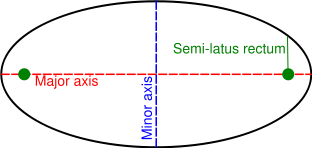
\includegraphics[width=80mm]{images/MajMinSemlatRec.png}
    \end{center}
    \linespread{1} 
	\caption[Ellipse notation]{
	Ellipse notation. When an $r$ for an orbiting object coincides with the semi-latus rectum, $\theta = \pi /2$.
	}
\label{EllipseNotation}
\end{figure}



\Table{
\hline

\textbf{Kepler's Law II} 	& A line joining a planet and the Sun sweeps  \\
					& out equal areas during equal intervals of time. \\
					& $\dfrac{dA}{dt} = \dfrac{1}{2}r^2 \dfrac{d \theta}{dt}$

\\ \hline
}

%%%%

\Table{
\hline

Period				& $P \cdot \dfrac{1}{2} r^2  \dfrac{d \theta}{dt} = \pi a b$

\\ \hline

Mean motion			& $n = 2 \pi / P$ \\
					& $r^2 \ d\theta = abn \ dt$

\\ \hline
}

%%%%

\Table{
\hline

\textbf{Kepler's Law III}

&
\MiniPg{.7}{
\center

The square of the orbital period of a planet is directly proportional to the cube of the semi-major axis of its orbit.

$\dfrac{T^2}{a^3} = \dfrac{4 \pi^2}{G(M + m)}$,

(Importantly) $T^2 \propto a^3 $
}

\\ \hline
}

%%%%

\Table{
\hline

Derive $T$ for circular orbit of & $ \dfrac{GMm}{r^2} = \dfrac{mv^2}{r} = m\omega^2r = \dfrac{mr(2 \pi)^2}{T^2} $ \\
planet about fixed mass $M$. & $T = \sqrt{\dfrac{4 \pi^2 r^3}{G M}}$

\\ \hline
}

%%%%%%%%%%%%%%%%%%%%%%%%%%%%%%%%%%%%%%%%%%%%%%%%%

\subsection{Three-dimensional particle dynamics}

%%%%%%%%%%%%%%%%%%%%%%%%%%%%%%%%%%%%%%%%%%%%%%%%%

\subsection{Lagrangian and Hamiltonian formalism}

\Table{
\hline

Lagrangian &

\MiniPg{.7}{\center $L = L(q,\dot{q},t) = T - V$}

\\ \hline

Euler-Lagrange equation & $\dfrac{\partial{L}}{\partial{q}} = \dfrac{d}{dt}\dfrac{\partial{L}}{\partial{\dot{q}}}$

\\ \hline

Action & $S = \int_{t_0}^{t_1} L(q(t),\dot{q}(t),t)dt$

\\ \hline
}

%%%%

\Table{
\hline

Principal of least action &
\MiniPg{.7}{
The path taken by the system between times $t_0$ and $t_1$ is the one for which the action is stationary (no change) to first order.
 $\delta S = 0$
}
    

\\ \hline

Conjugate momentum & $p = \dfrac{\partial L}{\partial \dot{q}}$

\\ \hline
}

%%%%

\Table{
\hline

Hamiltonian & $H = p\dot{q} - L = T + V$
 
  \\ \hline

\MiniPg{.3}{

Canonical Hamiltonian equations of motion

}
& 
\MiniPg{.7}{
\center
$\dfrac{\partial H}{\partial q} = - \dot{p}, \hspace{1cm} \dfrac{\partial H}{\partial p} = \dot{q}, \hspace{1cm} \dfrac{\partial H}{\partial t} = - \dfrac{\partial L}{\partial t} $
}
 
\\ \hline
}

%%%%%%%%%%%%%%%%%%%%%%%%%%%%%%%%%%%%%%

\subsection{Noninertial reference frames}

\Table{
\hline

Coriolis Force

&

\MiniPg{.7}{
\center
$\bold{F}_{coriolis} = -2m\pmb{\omega} \times (\bold{v}_{in \ rotating \ frame})$

Mnemonic: Coriolis makes it hard \textbf{2 mov} straight. (Steven Byrnes)
}

\\ \hline

Centrifugal Force

&

$ \bold{F}_{centrifugal} = -m\pmb{\omega} \times (\pmb{\omega} \times \pmb{r})$
 
 \\ \hline
}

%%%%%%%%%%%%%%%%%%%%%%%%%%%%%%%%%%%%%%

\subsection{Elementary topics in fluid dynamics}
\Table{
\hline

\MiniPg{.4}{
Bernoulli's Equation for fluid flow (Incompressible, nonviscous, laminar flow)
}

& 

$p + \rho g y + \dfrac{1}{2} \rho v^2 = constant$

\\ \hline

Incompressible flow

&

\MiniPg{.6}{\center

$\nabla \cdot \bold{u} = 0$, where $\bold{u}$ is the flow velocity. For a pipe this infers $\bold{A} \cdot \bold{u}_{\bot} = \textrm{(cross-sectional area)} \times \textrm{(velocity)} = constant$.
}


\\ \hline
}
%%%%

\Table{
\hline

Buoyancy force

&

$B = \rho_{fluid} V_{disp} g$

%\\ \hline
%    
%    Net force on object in fluid
%    
%    &
%    
%    $F_{\textrm{net}} = 

\\ \hline
}




\section{Electromagnetism}
(such as electrostatics, currents and DC
circuits, magnetic fields in free space,
Lorentz force, induction, Maxwell’s
equations and their applications,
electromagnetic waves, AC circuits,
magnetic and electric fields in matter)

\subsection{Electrostatics}
\Table{
\hline

$\epsilon$ is called... 	& permittivity %\\
%and has units ...		& Farads per meter (F/m) = 

\\ \hline

$\mu$ is called & permeability

\\ \hline

Gauss's Law & Flux $\Phi \equiv \oint \bold{E} \cdot d\bold{a} = Q_{enc} / \epsilon_0 \Leftrightarrow $ M.E. I

\\ \hline
}

%%%%

\Table{
\hline

E-field for sphere of radius R with 	& $E_{inside} = \dfrac{Q}{4 \pi \epsilon_0} \dfrac{r}{R^3}$ \\
uniformly distributed charge Q		& $E_{outside} = \dfrac{Q}{4 \pi \epsilon_0} \dfrac{1}{r^2}$

\\ \hline

Electric Potential	& $ V(\bold{a}) = - \int_0^a \bold{E}(\bold{r}) \cdot d\bold{l} $\\
				& $ V(a) - V(b) = \int_a^b \bold{E}(\bold{r}) \cdot d \bold{l} $
				
\\ \hline

Energy of a point charge & $W=QV$

\\ \hline
}

%%%%

\Table{
\hline

Energy of a collection of point charges 	& $ U = \dfrac{1}{8 \pi \epsilon_0} \sum_{j=0}^n \sum_{i=0, i\neq j}^{n} \dfrac{q_i q_j}{r_{if}} $ \\
								& $ U = \dfrac{1}{2} \sum_{all \ i} V_{due \ to \ others} (r_i)q_i $.

\\ \hline

\MiniPg{.4}{

\center

Energy of a continuous distribution of charge

}

&


\MiniPg{.6}{
\center

$W = \dfrac{1}{2} \int_V \rho V d \tau = \dfrac{\epsilon_0}{2} \int_{all space} E^2 d\tau $.

}

\\ \hline

Energy density of $E$ field

&

$\eta_E = \dfrac{1}{2}\epsilon E^2$	

\\ \hline
}

%%%%

\Table{
\hline

\MiniPg{.3}{
Conductor:  $\bold{E}_{inside} $, $\rho_{inside} $, $V(r) = $, $\hat{E}_{surface} $
}

&

\MiniPg{.7}{

 $\bold{E}_{inside} = \bold{0} \ \ \ \ \ \ \rho_{inside} = 0 \ \ \ \ \ \ V(r) = constant \ \ \ \ \ \ \hat{E}_{surface}  = \bot_{surface}$
}

\\ \hline
}

%%%%

\Table{
\hline
			& $\bold{E} (\bold{r}) = \dfrac{1}{4\pi \epsilon_0} \iiint_{volume} \dfrac{1}{R^2} \rho (\bold{r}') d\tau' \hat R$ \\
Coulomb's Law	& $\bold{E} (\bold{r}) = \dfrac{1}{4\pi \epsilon_0} \iint_{surface} \dfrac{1}{R^2} \sigma (\bold{r}') da' \hat R$ \\
			&  $\bold{E} (\bold{r}) = \dfrac{1}{4\pi \epsilon_0} \int_{line} \dfrac{1}{R^2} \lambda (\bold{r}') dl' \hat R$

\\ \hline

Coulomb Potential	&  $V (\bold{r}) = \dfrac{1}{4\pi \epsilon_0} \int \dfrac{1}{R} \rho (\bold{r}') d\tau' $

\\ \hline

}

%%%%

\Table{
\hline

Poisson's Equation	& $\nabla^2V = -\rho / \epsilon_0$ \\
Laplace's Equation	& $\nabla^2V = 0 $ 

\\ \hline

}


%%%%

\Table{
\hline


\begin{minipage}{.3\textwidth}
      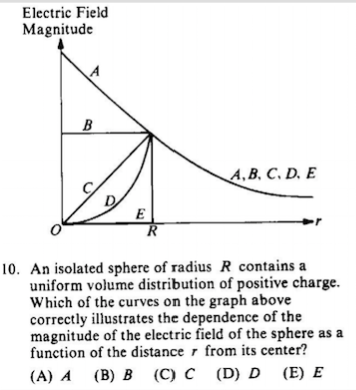
\includegraphics[width=\linewidth, height=60mm]{images/ChargeSphereUniform.png}
      \tiny \url{GR8677}
    \end{minipage}

& C

\\ \hline

Given $R$ and either $Q$ or $\rho$ find & $E(r<R) = \dfrac{Qr}{4 \pi \epsilon_0 R^3} = \dfrac{\rho r}{3 \epsilon_0} $ \\


E-field inside sphere and & \\


 outside sphere & $E(r>R) = \dfrac{Q}{4 \pi \epsilon_0 r^2} = \dfrac{\rho R^3}{3 \epsilon_0 r^2} $

\\ \hline

}

%%%%%

\Table{
\hline

Griffith's triangle of $\rho, V \& \bold{E}$ &

\begin{minipage}{.4\textwidth}
      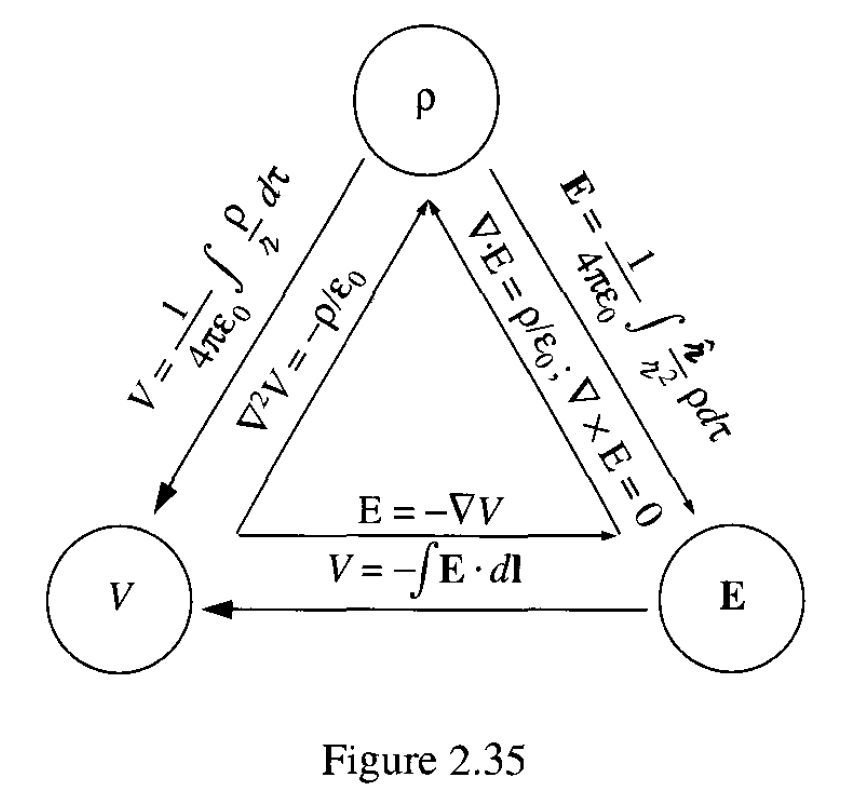
\includegraphics[width=\linewidth, height=60mm]{images/GriffithsTriangle.png}
      \tiny \textit{Introduction to Electrodynamics}, Griffiths
    \end{minipage}
    
\\ \hline
}

%%%%

\Table{
\hline

\MiniPg{.3}{

Electric potential for multipole expansion (far field)

}

&

\MiniPg{.7}{

\GraphicWHN{.76}{.2}{Mulitpole.png}
\center

\small Fig. 3.27 in Griffiths, \textit{Introduction to Electrodynamics}

}

\\ \hline
}

%%%%

\Table{
\hline

\MiniPg{.3}{

Electric dipole moment

}

&

\MiniPg{.7}{
\center

$\bold{p} \equiv \int \bold{r}' \rho{\bold{r}'} \, d\tau'$

For point charges, $\bold{p} = \sum_{i = 1}^{n} q_i \bold{r}_i'$.

}

\\ \hline
}

%%%%

\Table{
\hline

\MiniPg{.3}{

Electric potential for dipole

}

&

\MiniPg{.7}{
\center

$V_{\textrm{dip}}(\bold{r}) = \dfrac{1}{4 \pi \epsilon_0 } \dfrac{ \bold{p} \cdot \bold{\hat{r}} }{r^2} = \dfrac{p \ \cos \theta}{4 \pi \epsilon_0 r^2}$.

}

\\ \hline
}

%%%%

\Table{
\hline

\MiniPg{.3}{

Electric field of a dipole

}

&

\MiniPg{.7}{
\center

$\bold{E}_{\textrm{dip}}(\bold{r}) = \dfrac{1}{4 \pi \epsilon_0} \dfrac{1}{r^3} [3(\bold{p} \cdot \bold{\hat{r}})\bold{\hat{r}} - \bold{p}]$.

$\bold{E}_{\textrm{dip}} (r, \theta) = \dfrac{p}{4 \pi \epsilon_0 r^3} (2 \cos \theta  \,\bold{\hat{r}} + \sin \theta \,\pmb{\hat{\theta}})$.

\GraphicWHN{.4}{.32}{Dipole.png}

\center
\small Fig. 3.36 from Griffiths, \textit{Introduction to Electrodynamics}

}

\\ \hline
}

%%%%%%%%%%%%%%%%%%%%%%%%%%%%%%%%%%%%%

\subsection{Capacitors}
\Table{
\hline

Capacitance & $C = \dfrac{q}{V}$

\\ \hline

Voltage/current relationship & $I(t) = C\dfrac{dV(t)}{dt}$

\\ \hline

Charging energy & $W_{\textrm{charging}} = \dfrac{1}{2} C V^2$

\\ \hline
}

%%%%

\Table{
\hline

Capacitance of a capacitor

& 

\MiniPg{.6}{

Mutual capacitance between two conducting plates, i.e. a regular capacitor, is given by

$C = \epsilon_r \epsilon_0 \dfrac{A}{d}$.

}

\\ \hline
}

%%%%%%%%%%%%%%%%%%%%%%%%%%%%%%%%%%%%%%%

\subsection{Currents and DC}
\Table{
\hline

Amperes = & Coulombs / second
 
 \\ \hline

Ohm's Law & $V=IR$

\\ \hline
}

%%%%

\Table{
\hline
 
Current in a wire of area $A$, & \\
velocity of charges $v$, & $I = v \rho A$ \\
 charge density $\rho$ &

\\ \hline
}

%%%%

\Table{
\hline

\MiniPg{.3}{Kirchoff's current law}

&

\MiniPg{.7}{

The algebraic sum of currents in a network of conductors meeting at a point is zero.

}

\\ \hline

\MiniPg{.3}{Kirchoff's voltage law}

&

\MiniPg{.7}{

The directed sum of the electrical potential differences (voltage) around any closed network is zero.

}

\\ \hline
}

%%%%

\Table{
\hline

RC circuit $V(t)$ where $V(0)=V_0$

&

\MiniPg{.6}{
\center

Start with Kirchoff's current law for a circuit consisting of just a capacitor and a resistor.

 $C\dfrac{dV}{dt} + \dfrac{V}{R} = 0$
 
Solve the DE.

$\boxed{ V(t) = V_0e^{-\frac{t}{RC}}}$

}

\\ \hline
}

%%%%

\Table{
\hline

RL circuit voltages across R and L

&

\MiniPg{.6}{ \center
 $V_L(t) = V e^{-t \frac{R}{L}} $
  
$V_R(t) =V(1 - e^{-t \frac{R}{L}})$
}
\\ \hline
}



%%%%%%%%%%%%%%%%%%%%%%%%%%%%%%%%%%%%%%%%



\subsection{Magnetic fields in free space}

\Table{
\hline

Biot-Savart Law & $\bold{B} = \dfrac{\mu_0}{4\pi} \int \dfrac{\bold{I} \times \hat R}{R^2} dl' = \dfrac{\mu_0 I}{4\pi} \int \dfrac{\bold{dl'} \times \hat R}{R^2} $

\\ \hline

Ampere's law	& $\oint \bold{B} \cdot d\bold{l} = \mu_0 I_{enc} $

\\ \hline
}

%%%%

\Table{
\hline

\MiniPg{.3}{

B-field for solenoid with $n$ turns per unit length and current $I$.

}

&

$\bold{B} = \mu_0 n I \hat z $

\\ \hline
}

%%%

\Table{
\hline

B-field for infinite wire

&

$B = \dfrac{\mu_0 I}{2 \pi r}$

\\ \hline
}

%%%%

\Table{
\hline

\begin{minipage}{.3\textwidth}

Field on axis of current loop.

General, $z=0$, and $z>>R$


\end{minipage}

& 

\MiniPg{.7}{
\GraphicWHN{.7}{.54}{MagCurLoop.png}

\center

\tiny \url{http://hyperphysics.phy-astr.gsu.edu/hbase/magnetic/curloo.html}

\large

$B = B_Z = \dfrac{\mu_0}{4 \pi} \dfrac{2 \pi R^2 I}{(z^2 +R^2)^{3/2}} =\boxed{\dfrac{\mu_0}{2} \dfrac{R^2 I}{(z^2 +R^2)^{3/2}}}$

If $z = 0$ then $\boxed{B = \dfrac{\mu_0 I}{2R} }$.

If $z>>R$ then $\boxed{B \approx \dfrac{\mu_0}{2} \dfrac{R^2 I}{z^3}}$

}

\\ \hline
}

%%%%

\Table{
\hline

Magnetic vector potential	& $\bold{B} = \bold{\nabla} \times \bold{A} 	$\\
					&$ \bold{A} \parallel  \bold{J} $ \\
					&$ \bold{A}(\bold{r}) = \dfrac{\mu_0}{4 \pi} \int \dfrac{\bold{J}(\bold{r}')}{R} d\tau' $ \\
					&$ \oint \bold{A} \cdot d \bold{l} = \Phi_B $

\\ \hline

}

%%%%

\Table{
\hline

\MiniPg{.3}{

Griffiths triangle for magnetostatics 

}

&

\MiniPg{.7}{

\GraphicWHN{.5}{.5}{MagTriangle.png}

\center
\small Griffiths, \textit{Introduction to Electrodynamics}

}

\\ \hline
}

%%%%

\Table{
\hline

\MiniPg{.3}{

Magnetic vector potential for magnetic dipole

}

&

\MiniPg{.7}{
\center

$ \bold{A}_{\textrm{dip}} (\bold{r}) = \dfrac{\mu_0}{4 \pi} \dfrac{\bold{m} \times \bold{\hat{r}}} {r^2} $

$\bold{A}_{\textrm{dip}} (\bold{r}) = \dfrac{\mu_0}{4 \pi} \dfrac{m \, \sin \theta}{r^2} \pmb{\hat{\phi}}$.

}

\\ \hline

Magnetic dipole moment

&

$\bold{m} \equiv I \int d\bold{a} = I \bold{a}$

\\ \hline
}

%%%%

\Table{
\hline

\MiniPg{.3}{

Magnetic field of magnetic dipole

}

&

\MiniPg{.7}{
\center

$\bold{B}_{\textrm{dip}}(\bold{r}) = \dfrac{\mu_0}{4 \pi} \dfrac{1}{r^3} [3( \bold{m} \cdot \bold{\hat{r}}) \bold{\hat{r}} - \bold{m}].$


$\bold{B}_{\textrm{dip}} (\bold{r}) = \dfrac{ \mu_0 m}{4 \pi r^3} (2 \cos \theta \bold{\hat{r}} + \sin \theta \pmb{\hat{ \theta}})$.

\GraphicWHN{.35}{.3}{MagDipole.png}

\center

\small Fig. 5.54 from Griffiths, \textit{Introduction to Electrodynamics}

}

\\ \hline
}

%%%%

\Table{
\hline

Potential energy associated with magnetic moment

& 

$U(\theta) = - \pmb{\mu} \cdot \bold{B}$

\\ \hline
}

%%%%

\Table{
\hline

Larmor precession

&

\MiniPg{.7}{
\center
$\pmb{\tau} = \pmb{\mu} \times \bold{B}$. This causes centripetal acceleration (think of the poles of the magnet).

\MPalign{

\dfrac{dL}{dt} &= \tau \\
 \dfrac{L \sin \theta d\phi}{dt} &= |\mu B \sin \theta| \\
 \omega_{\textrm{precession}} &= \dfrac{\mu B}{L}
 
}
}

\\ \hline
}

%%%%%%%%%%%%%%%%%%%%%%%%%%%

\subsection{Lorentz force}

\Table{
\hline

The Lorentz Force & $ \bold{F} = q(\bold{E} + \bold{v} \times \bold{B})$

\\ \hline
}

%%%%

\Table{
\hline
\MiniPg{.3}
{
Magnetic force on a current carrying wire of length $l$ and current $I$ in a field $\bold{B}$
}
&
\MiniPg{.6}
{

\center

$\bold{F} = q \bold{v} \times \bold{B} = qvB (\hat{v} \times \hat{B}) = q\dfrac{l}{t}B (\hat{v} \times \hat{B})  = \dfrac{q}{t} l B (\hat{v} \times \hat{B}) = \boxed{ I l B (\hat{v} \times \hat{B}) }$

%\begin{tabular}{c c}
%$\bold{F}$&$= q \bold{v} \times \bold{B}$ \\
%	 &$= qvB (\hat{v} \times \hat{B})$ \\
%	 &$= q\dfrac{l}{t}B (\hat{v} \times \hat{B}) $\\
%	 &$= \dfrac{q}{t} l B (\hat{v} \times \hat{B})$ \\
%	 &$= \boxed{ I l B (\hat{v} \times \hat{B}) }$
% \end{tabular}

}
 
 \\ \hline
}

%%%%

\Table{
\hline

\MiniPg{.25}{
Larmor radius, cyclotron or gyroradius rather
}

&

\MiniPg{.75}{
\center

A charged particle traveling perpendicular to a magnetic field will gyrate in a circle whose area vector is parallel to the direction of travel resulting in a corkscrew-like trajectory. The radius of gyration is determined by considering the Lorentz force on such a particle.

$\dfrac{mv_{\bot}^2}{r_g} = |q|v_{\bot}B \Rightarrow \boxed{r_g = \dfrac{mv_{\bot}}{|q|B}}$

}

\\ \hline
}

%%%%

\Table{
\hline

Cyclotron frequency

&

\MiniPg{.7}{

\MPalign{
T_g &= \dfrac{2 \pi r_g}{v_{\bot}} = \dfrac{2 \pi}{v_{\bot}} \dfrac{mv_{\bot}}{|q|B} = \dfrac{2 \pi m}{|q|B} \\
f_g &= \dfrac{|q|B}{2 \pi m} \\
\omega_g &= \dfrac{|q|B}{m}
}

}


\\ \hline
}



%%%%%%%%%%%%%%%%%%%%%%%%%%%%%%%


\subsection{Induction}
\Table{
\hline

Faraday's/Lenz's law

&

\MiniPg{.6}{
\center
If an induced current flows, its direction is always such that it will oppose the change which produced it.

$\varepsilon = -\dfrac{d \Phi_B}{dt}$

}

\\ \hline
}

%%%%

\Table{
\hline

\MiniPg{.4}{

EMF for tightly wound coil of wire

}

&

$\varepsilon = -N\dfrac{d \Phi_B}{dt}$

 \\ \hline

Inductance & $L \equiv \dfrac{\Phi_B}{I}$

\\ \hline
}

%%%%

\Table{
\hline

Voltage, given inductance & $V = \dfrac{d}{dt}(LI) = L \dfrac{dI}{dt}$

\\ \hline

Energy in an inductor

&

$W = \int P \ dt = \int IV \ dt = \int I L \dfrac{dI}{dt} dt = L \int I \ dI = \boxed{\dfrac{1}{2} L I^2}.$

\\ \hline
}

%%%%

\Table{
\hline

\MiniPg{.3}{
Energy density in magnetic field
}
&

\MiniPg{.7}{
\center

$\eta_B =  \dfrac{W}{V}  = \dfrac{ \frac{1}{2} LI^2  }{A l} = \dfrac{1}{2} \dfrac{\frac{\Phi_B}{I} I^2}{A l} = \dfrac{1}{2} \dfrac{BAI}{Al}  = \dfrac{1}{2} \dfrac{BI}{l} .$


But in a solenoid, we have $\bold{B} = \mu n I \hat{z} = \dfrac{\mu I}{l}$, so $\dfrac{I}{l} = \dfrac{B}{\mu}$. Therefore, $\boxed{\eta_B = \dfrac{1}{2} \dfrac{B^2}{\mu}}$.

}

\\ \hline
}

%%%%%%%%%%%%%%%%%%%%%%%


\subsection{Maxwell's Equations}

\Table{
\hline

Maxwell's equations 	& $\pmb{\nabla} \cdot \bold{E} = \rho / \epsilon_0 $ (Gauss) \\
in vacuum. 		& $\pmb{\nabla} \cdot \bold{B} = 0 $ \\
Differential form	& $\pmb{\nabla} \times \bold{E} = -\dfrac{\partial \bold{B}}{\partial t} $ (Faraday) \\
				& $\pmb{\nabla} \times \bold{B} = \mu_0\bold{J} + \epsilon_0 \mu_0 \dfrac{\partial \bold{E}}{\partial t} $ (Ampere)

\\ \hline
}

%%%%
\Table{
\hline

Maxwell's equations 	& $\oiint\limits_{\partial \Omega} \bold{E} \cdot d\bold{S} = \dfrac{1}{\epsilon_0} \iiint_\Omega \rho dV$ (Gauss) \\
in vacuum. 		& $\oiint_{\partial \Omega} \bold{B} \cdot d\bold{S} = 0$ \\
Integral form		& $\oint_{\partial \Sigma} \bold{E} \cdot d\bold{l} = -\dfrac{d}{dt} \iint_\Sigma \bold{B} \cdot d\bold{S}$ (Faraday) \\
				& $ \oint_{\partial \Sigma} \bold{B} \cdot d \bold{l} = \mu_0 \iint_\Sigma \bold{J} \cdot d\bold{S} + \mu_0\epsilon_0 \dfrac{d}{dt} \iint_\Sigma \bold{E} \cdot d\bold{S} $ (Ampere)

\\ \hline
}

%%%%
\Table{
\hline

\MiniPg{.3}{
\center

Maxwell's equations in matter.
Differential form
}
&
\MiniPg{.7}{
\center
$\pmb{\nabla} \cdot \bold{D} = \rho_{free}  $ (Gauss), \, \, \, 
\small $D = \epsilon_0 E + P, \, \, \, \, \, D = \epsilon E$

\large

$\pmb{\nabla} \cdot \bold{B} = 0 $ \\

$\pmb{\nabla} \times \bold{E} = -\dfrac{\partial \bold{B}}{\partial t} $ (Faraday) \\

$\pmb{\nabla} \times \bold{H} = \bold{J}_{free} + \dfrac{\partial \bold{D}}{\partial t} $ (Ampere), \, \, \,
\small $B = \mu_0(H + M), \, \, \, \, \, B = \mu H$
\large

}
\\ \hline
}


\Table{
\hline

Maxwell's equations 	& $\oiint\limits_{\partial \Omega} \bold{D} \cdot d\bold{S} = \iiint_\Omega \rho_{free} dV$ (Gauss) \\
in matter. 		& $\oiint_{\partial \Omega} \bold{B} \cdot d\bold{S} = 0$ \\
Integral form		& $\oint_{\partial \Sigma} \bold{E} \cdot d\bold{l} = -\dfrac{d}{dt} \iint_\Sigma \bold{B} \cdot d\bold{S}$ (Faraday) \\
				& $ \oint_{\partial \Sigma} \bold{H} \cdot d \bold{l} = \iint_\Sigma \bold{J}_{free} \cdot d\bold{S} + \dfrac{d}{dt} \iint_\Sigma \bold{D} \cdot d\bold{S} $ (Ampere)

\\ \hline
}

\Table{
\hline
Boundary conditions

&
\MiniPg{.7}{

\MPalign{

(i)&  D^\bot_1 - D^\bot_2 = \sigma_f \\

(ii)& B^\bot_1 -B^\bot_2 = 0 \\

(iii)&  \bold{E^{||}_1} - \bold{E^{||}_2} = 0 \\

(iv)&  \bold{H^{||}_1} - \bold{H^{||}_2} = \bold{K}_f \times \bold{ \hat{n}}
}

}

 \\ \hline
}

%======================================================%

\subsection{EM Waves}
\Table{
\hline
\MiniPg{.2}{ The whole EM wave spiel}

&

\MiniPg{.8}{
		\center
		For E-wave, curl Faraday.
		
		$\nabla \times \nabla \times \bold{E} = \nabla \times \Big(-\dfrac{\partial B}{\partial t} \Big)$ 

		$\nabla (\nabla \cdot \bold{E} ) - \nabla^2 \bold{E}  = -\dfrac{\partial}{\partial t} (\nabla \times \bold{B}) $
		
		Substitute Gaussian and Amperian terms.
		
		$\nabla \Big(\dfrac{\rho}{\epsilon_0}\Big) - \nabla^2 \bold{E}  = -\dfrac{\partial}{\partial t} \Big(\mu_0\bold{J} + \epsilon_0 \mu_0 \dfrac{\partial \bold{E}}{\partial t}\Big) $
		
		$\rho = 0$ and $\bold{J} = 0$, therefore  $\boxed{\nabla^2 \bold{E} = \epsilon_0 \mu_0 \dfrac{\partial^2 \bold{E} }{ \partial t^2} = \dfrac{1}{c^2}\dfrac{\partial^2 \bold{E} }{ \partial t^2} }$
		
		For B-wave, similar, but start with curling Ampere's Law.
	}
	
\\ \hline
}

%%%%

\Table{
\hline

speed of light in vacuum & $c = \dfrac{1}{\sqrt{\mu_0 \epsilon_0}} = 3 \times 10^8$ m/s 

\\ \hline

speed of light in medium, $v= $& $\dfrac{1}{\sqrt{\mu \epsilon}} = \dfrac{c}{\sqrt{\epsilon_R \mu_R}}$, where $\mu = \mu_R \mu_0$ and likewise for $\epsilon$

 \\ \hline

 Plane wave solutions & $E = E_m \sin(kx - \omega t)$ and $ B = B_m\sin(kx - \omega t)$
 
 \\ \hline
}

%%%%

\Table{
\hline
 
 \MiniPg{.3}{
 Relation of $E_m$ and $B_m$ magnitudes
 }
 
 &
 
 \MiniPg{.7}{ Plug plane wave solutions into Ampere or Faraday and find that
 \center
 $\dfrac{E_m}{B_m} = \dfrac{\omega}{k} = c$
 
 }
 
 \\ \hline
}

%%%%

\Table{
\hline

\MiniPg{.3}{

Energy in the E and B fields for plane wave

}

&

\MiniPg{.7}{
\center


Recall the energy densities $\eta_E = \dfrac{1}{2} \epsilon_0 E^2$ and $\eta_B = \dfrac{1}{2} \dfrac{B^2}{\mu_0}$.

$\dfrac{\eta_E}{\eta_B} = \dfrac{\mu_0 \epsilon_0 E^2}{B^2} = \dfrac{E^2}{c^2 B^2}$.

From above, $E = cB$. Therefore $\eta_E = \eta_B$ for an EM wave; the energy carried in the E-field is equal to the energy carried in the B-field.

}

\\ \hline
}

%%%%

\Table{
\hline

Poynting Vector

& 

\MiniPg{.6}{
\center
	
$\bold{S} = \dfrac{1}{\mu_0} \bold{E} \times \bold{B}$

$S = \dfrac{1}{\mu_0} EB = \dfrac{c}{\mu_0} B^2 = \dfrac{1}{c\mu_0} E^2 $

}

\\ \hline
}

%%%%

\Table{
\hline

Average intensity

&

$\overline{S} = \dfrac{1}{c \mu_0} E^2_m \overline{\sin^2(kx - \omega t)} = \dfrac{1}{c \mu_0} \dfrac{E_m^2}{2}$
	
\\ \hline

\MiniPg{.4}{

Power radiated by a non relativistic point charge as it accelerates

}

&

\MiniPg{.6}{
\center

Larmor formula

$P = \dfrac{2}{3}\dfrac{q^2 a^2}{4 \pi \epsilon_0 c^3} = \dfrac{q^2 a^2}{6 \pi \epsilon_0 c^3} $.

}


	
\\ \hline
}


%%%%%

\Table{
\hline

\MiniPg{.4}{
Application of boundary conditions for reflection of a wave incident to a conducting surface
}

&

\MiniPg{.6}{

(i) Incident wave, $E^\bot = 0$ on both sides $\rightarrow \, \sigma_f = 0$ 

(ii) Automatically satisfied because $B^\bot = 0$

(iii) $\tilde{E}_{0_I} + \tilde{E}_{0_R} = \tilde{E}_{0_T}$

(iv)

\GraphicWHN{1}{.6}{ivEMWaveCond.png}

Wave is reflected with $\pi$ phase shift. Also, from the last equation above, $\tilde{B}_{0_R} = -\tilde{B}_{0_I}, \ \ \tilde{B}_{0_T} = 0$. From the first expression it follows that the magnetic field at the surface is twice the magnitude of either incident or reflected. 

\tiny \textit{Introduction to Electrodynamics}, Griffiths

}

\\ \hline

}

%%%%

\Table{
\hline

Oscillating electric dipole

&

\MiniPg{.6}{
\center

$q(t) = q_0 \cos(\omega t) \;\;\;\;\;\;\; \bold{p}(t) = p_0 \cos(\omega t) \bold{\hat{z}} \;\;\;\;\;\;\; p_0 \equiv q_0 d.$

}

\\ \hline
}

%%%%

\Table{
\hline

\MiniPg{.4}{

Approximations for oscillating electric dipole far from the source (such that it can be approximated as a plane wave)

}

&

\MiniPg{.6}{
\center

Approximation 1: $d \ll r$.

Approximation 2: $d \ll \dfrac{c}{\omega} = \dfrac{\lambda}{2 \pi}$.

Approximation 3: $r  \gg  \dfrac{c}{\omega} = \dfrac{\lambda}{2 \pi}$.


}

\\ \hline
}

%%%%
\Table{
\hline

\MiniPg{.4}{

Electric potential far from oscillating electric dipole

}

&

\MiniPg{.6}{
\center

$V(r, \theta, t) = - \dfrac{ p_0 \omega}{4 \pi \epsilon_0 c} \BigP{ \dfrac{\cos \theta}{r} } \sin [\omega(t - r/c)]$

}

\\ \hline
}

%%%%

\Table{
\hline

\MiniPg{.4}{

Magnetic vector potential far from oscillating electric dipole on the z-axis

}

& 

\MiniPg{.6}{
\center

$\bold{A}(r, \theta, t)  = - \dfrac{\mu_0 p_0 \omega}{4 \pi r} \sin [ \omega ( t - r/c) ] \bold{\hat{z}}$

}

\\ \hline
}

%%%%

\Table{
\hline

\MiniPg{.4}{

Electric field far from oscillating electric dipole

}

&

\MiniPg{.6}{
\center

$\bold{E} = -\nabla V - \dfrac{ \partial \bold{A}}{ \partial t} = -\dfrac{\mu_0 p_0 \omega^2}{4\pi} \BigP{\dfrac{\sin \theta}{r}} \cos [\omega(t - r/c)] \pmb{\hat{\theta}}$

}

\\ \hline
}

%%%%

\Table{
\hline

\MiniPg{.4}{

Magnetic field far from oscillating electric dipole

}

&

$\bold{B} = \nabla \times \bold{A} = - \dfrac{\mu_0 p_0 \omega^2}{4 \pi c} \BigP{\dfrac{\sin \theta}{r}} \cos [\omega(t - r/c)]\pmb{\hat{\phi}}$

\\ \hline
}


%%%%%%%%%%%%%%%%%%%%%%%%%%%%%%%%%%%%%%%%%


\subsection{AC circuits}
\Table{
\hline

\begin{minipage}{.3\textwidth}

Second-order DE for RLC circuits

\end{minipage}

& 

\begin{minipage}{.6\textwidth}
\center

Kirchoff's voltage law:

$V_R + V_L + V_C = V(t) $

$RI(t) + L\dfrac{dI}{dt} + \dfrac{1}{C}\int_{-\infty}^{\tau = 1} I(\tau) \, d\tau = V(t)$

In case of $\dfrac{dV}{dt} = 0$, we differentiate and rearrange

$L\dfrac{d^2 I(t)}{dt^2} + R\dfrac{d I(t)}{dt}  + \dfrac{1}{C}I(t) = 0$

\end{minipage}

\\ \hline
}

%%%%

\Table{
\hline

Resonant frequency RLC & 
\MiniPg{.65}{\center
$\omega_0 = \dfrac{1}{\sqrt{LC}}$
}

\\ \hline
}

%%%%

\Table{
\hline

\MiniPg{.3}{
Impedance matching
}

&

 \begin{minipage}{.7\textwidth}

To maximize power transfer, $Z_S = Z_L^*$, where $Z_S$ is the complex source impedance, and $Z_L$ is the load impedance.

To minimize reflection in a transmission line where $Z_S$ is the characteristic impedance of the line, $Z_S=Z_L$.

\end{minipage}

\\ \hline
}

%%%%

\Table{
\hline

\begin{minipage}{.3\textwidth}
High- and Low-pass filters. One of each with a capacitor. One of each with an inductor.
\end{minipage}

&

\begin{minipage}{.6\textwidth}
      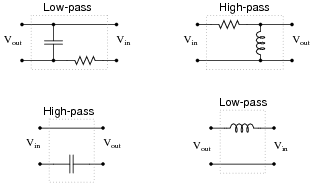
\includegraphics[width=\linewidth, height=50mm]{images/HiLoPass.png}
      \tiny \url{http://www.learningelectronics.net/images/quiz/00615x02.png}
            \end{minipage}

 \\ \hline
}

%%%%%%%%%%%%%%%%%%%%%%%%%%%%%%%%%%%%%%%

\subsection{Magnetic and electric fields in matter}
\Table{
\hline

Dipole moment & $ \bold{p} = \alpha\bold{E} $, where $\alpha$ is atomic polarizability.

\\ \hline

Polarization & $\bold{P} = \bold{p} \ / $ unit volume

\\ \hline

Bound charge 	& $ \sigma_b = \bold{P} \cdot \hat n,  \ \ \ \ \ \rho_b = - \pmb{\nabla} \cdot \bold{P}$

\\ \hline

Electric displacement field & $\bold{D} = \epsilon_0 \bold{E} + \bold{P} = \epsilon \bold{E}$

 \\ \hline
}

%%%%

\Table{
\hline

Gauss's Law in L.D.

&

\MiniPg{.6}{
\center

$\epsilon_0 \nabla \cdot \bold{E} = \rho = \rho_b + \rho_f = - \nabla \cdot \bold{P} + \rho_f$

$\nabla \cdot (\epsilon_0 \bold{E} + \bold{P}) = \nabla \cdot \bold{D} = \rho_f$

}

\\ \hline
}

%%%%

\Table{
\hline

Polarization in linear dielectrics 	& $\bold{P} = \epsilon_0 \chi_e \bold{E}$, where $\chi_e$ is the electric susceptibility.

\\ \hline

$ \bold{D} $ in terms of $\chi_e$ 	& $\bold{D} = \epsilon_0 (1 + \chi_e)\bold{E} = \epsilon \bold{E}$, where permittivity $\epsilon \equiv \epsilon_0 (1 + \chi_e) $

\\ \hline

Dielectric constant	& $\epsilon_r \equiv 1 + \chi_e \equiv \epsilon / \epsilon_0 $, (a.k.a. relative permittivity)

\\ \hline
}

%%%%

\Table{
\hline

$\bold{E} $ in dielectric  filled space & 
\MiniPg{.6}{\center
$\dfrac{1}{\epsilon_r} \bold{E}_{vac}$
}
\\ \hline

E-field in capacitor with dielectric

&

$E = \Delta V / d$

\\ \hline

Capacitance with linear dielectric

&

$C = \epsilon_r C_{\textrm{vac}}$

\\ \hline
}

%%%%

\Table{
\hline

Boundary conditions 	& $\epsilon_aE_a^\bot -\epsilon_bE_b^\bot = \sigma_f $ \\
				& $ V(a) = V(b) $
				
\\ \hline
}

%%%%%%%%%%%%%

\Table{
\hline

Magnetic dipole moment	& $\bold{m} = I \bold{a} $

\\ \hline

Magnetization	& $\bold{M} \equiv \bold{m} / $ unit volume

\\ \hline
}

%%%%

\Table{
\hline

$H$ field	& $\bold{H} \equiv \dfrac{1}{\mu_0} \bold{B} - \bold{M} $\\
		& $\pmb{\nabla} \times \bold{H} = \bold{J}_f $ \\
		& $\pmb{\nabla} \cdot \bold{H} = -\pmb{\nabla} \cdot \bold{M} $\\
		& Generally, $\bold{H} \parallel \bold{B} \parallel \bold{M} $.

\\ \hline
}

%%%%

\Table{
\hline

Linear magnetic materials	& $\bold{M} = \chi_m \bold{H} $ \\
					& where $\chi_m = $ magnetic susceptibility.

\\ \hline
}

%%%%

\Table{
\hline

B-field in linear	mag. material 	& $\bold{B} = \mu_0(1+\chi_m)\bold{H} = \mu \bold{H} $ \\
						& where $\mu \equiv \mu_0(1+\chi_m) = $ magnetic permeability. \\
						& $B_{material} = \dfrac{\mu}{\mu_0}B_{vacuum} = \mu_r B_{vacuum} $ \\
						& where $\mu_r \equiv \mu / \mu_0 = $ relative permeability.


\\ \hline
}

%%%%%%%%%%%%%

\Table{
\hline

Hall effect & 
\begin{minipage}{.55\textwidth}
      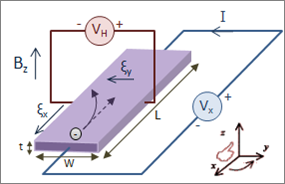
\includegraphics[width=\linewidth, height=50mm]{images/HallEffect.png}
            \end{minipage}
            \\
            &
            \tiny \url{https://en.wikipedia.org/wiki/Hall_effect}

\\ \hline
}

%%%%

\Table{
\hline

Hall voltage for electrons & $V_H = v_xB_zw $ and $I_x = ntw(-vx)(-e) $\\
& $V_H = \dfrac{I_x B_z}{nte}$

\\ \hline
}

%%%%

\Table{
\hline

Hall coefficient for electrons & $R_H = \dfrac{E_y}{j_x B} = \dfrac{V_H t}{I B} = - \dfrac{1}{ne}$ \\
& $[R_H] = $m$^3$/C

\\ \hline
}





\section{Optics and Wave Phenomena}
(such as wave properties, superposition,
interference, diffraction,
geometrical optics, polarization,
Doppler effect)

\subsection{Wave properties}

\Table{
\hline

The wave equation & $\dfrac{\partial^2 u}{\partial t^2} = c^2 \nabla^2 u.$

\\ \hline

General solution & $u(x,t) = A \sin(kx - \omega t) + B \cos(dx - \omega t).$

\\ \hline

$c$ & $c = \omega / k$

\\ \hline
}

%%%%

\Table{
\hline

\textbf{General wave function} $f(x,t,k,\omega) = $ & $A \sin (kx \pm \omega t) $

\\ \hline

wave function $f(x,t,\lambda,T) = $ & $A \sin 2\pi (\dfrac{x}{\lambda} \pm \dfrac{t}{T})$

\\ \hline
}

%%%%

\Table{
\hline

Amplitude & $A$

\\ \hline

Period & $T$

\\ \hline
}

%%%%

\Table{
\hline

Direction &

\MiniPg{.7}{ The $\sin$ function preserves a sine wave form as it traverses $x$ and $t$. The argument must remain constant:  $kx \pm \omega t = constant$. In order to preserve this, must $x$ increase or decrease as $t$ increases? Depends on the $\pm$ }

\\ \hline
}

%%%%

\Table{
\hline

$k = $	& $k = 2\pi / \lambda $

\\ \hline

$\omega = $	& $= \omega = 2 \pi f = 2 \pi / T $

\\ \hline
}

%%%%

\Table{
\hline

Phase velocity	& $v_{ph} = \omega / k  = \lambda / T$

\\ \hline

Group velocity	& $v_g = \dfrac{\partial \omega}{\partial k} $

\\ \hline
}

%%%%%%%%%%%%%%%%%%%%%%%%%%%%%%%%%%%%%%%%%%%

\subsection{Waves on a string}
\Table{
\hline

Characteristic impedance of a string & $Z = \mu c$ where $\mu$ is the mass \\
							& per unit length \& c is the wave speed.

\\ \hline
}

If you want to be super in the know about transverse waves on strings, check this out: \url{http://www.people.fas.harvard.edu/~djmorin/waves/transverse.pdf }

%\subsection{Superposition}


%%%%%%%%%%%%%%%%%%%%%%%%%%%%%%%%%%%%%%

\subsection{Interference}
\Table{
\hline

\MiniPg{.4}{

Michelson Interferometer equation relating distance (moved perhaps), number of fringes, and wavelength.

}

&

\MiniPg{.6}{
$2d = m \lambda$, where $m$ is the number of fringes. The factor of 2 comes from the fact that the light crosses the same distance twice. See GR9277 \#96 for an interesting problem.
}
\\ \hline
}

%%%%%%%%%%%%%%%%

\subsubsection{Two waves at the same speed}
\Table{
\hline

Sine waves in  & Same $\rightarrow$ interference. Opposite $\rightarrow$ standing. \\
same/opp. direction & 

\\ \hline

Constructive if & $\phi_1 = \phi_2$ \\
Destructive if & $|\phi_1 - \phi_2| = \pi$

\\ \hline
}

%%%%

\Table{
\hline

Standing wave  & $u(x,t) = A \sin(kx - \omega t) + A \sin (kx + \omega t) $ \\
equation					& $= 2 A \sin(kx)\, \cos(\omega t).$

\\ \hline
}

%%%%%

\Table{
\hline

Condition for nodes & $u(x,t) = 0 \,\, \Rightarrow \,\, kx = n\pi$

\\ \hline

Condition for antinodes & $u(x,t) = \textrm{max.} = 2A  \,\, \Rightarrow \,\, kx = \pi/2 + n\pi$

\\ \hline
}

%%%%

\Table{
\hline

Condition for beats & Same direction, different frequency

\\ \hline

Equation for beats & $u(x,t) = A \sin(k_1x - \omega_1 t) + A \sin (k_2x + \omega_2 t) $ \\
			& $=2A \sin \Big[ \dfrac{(k_1 + k_2)x}{2} - \dfrac{(\omega_1 + \omega_2)t}{2} \Big]\cos \Big[ \dfrac{(k_1 - k_2)x}{2} - \dfrac{(\omega_1 - \omega_2)t}{2} \Big]$
			
\\ \hline

Beat frequency & $\omega_{beat} = |\omega_1 - \omega_2|$

\\ \hline
}

%%%%%%%%%%%%%%%%%%%%%%%%%%%%%%%%

\subsubsection{Holography}
\Table{
\hline

Holographs & \begin{minipage}{.6\textwidth}
 encode the light field as an interference pattern, recording phase and amplitude.
 \end{minipage}
 
 \\ \hline
}

%%%

\Table{
\hline
 
 Holograph construction
 
 &
 
 \begin{minipage}{.5\textwidth}
      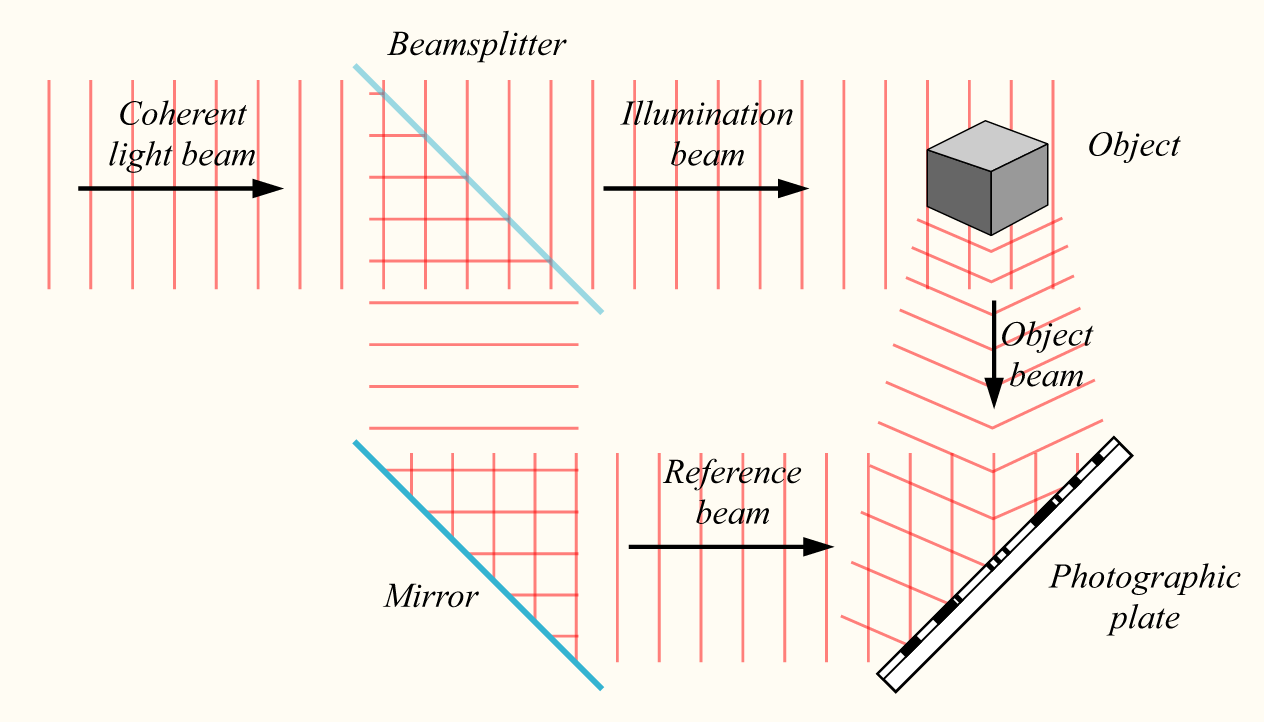
\includegraphics[width=\linewidth, height=45mm]{images/HoloConstruct.png}
      
       \end{minipage}
       
\\ \hline
}

%%%%

\Table{
\hline

 Holograph construction
 
 &
 
 \begin{minipage}{.3\textwidth}
      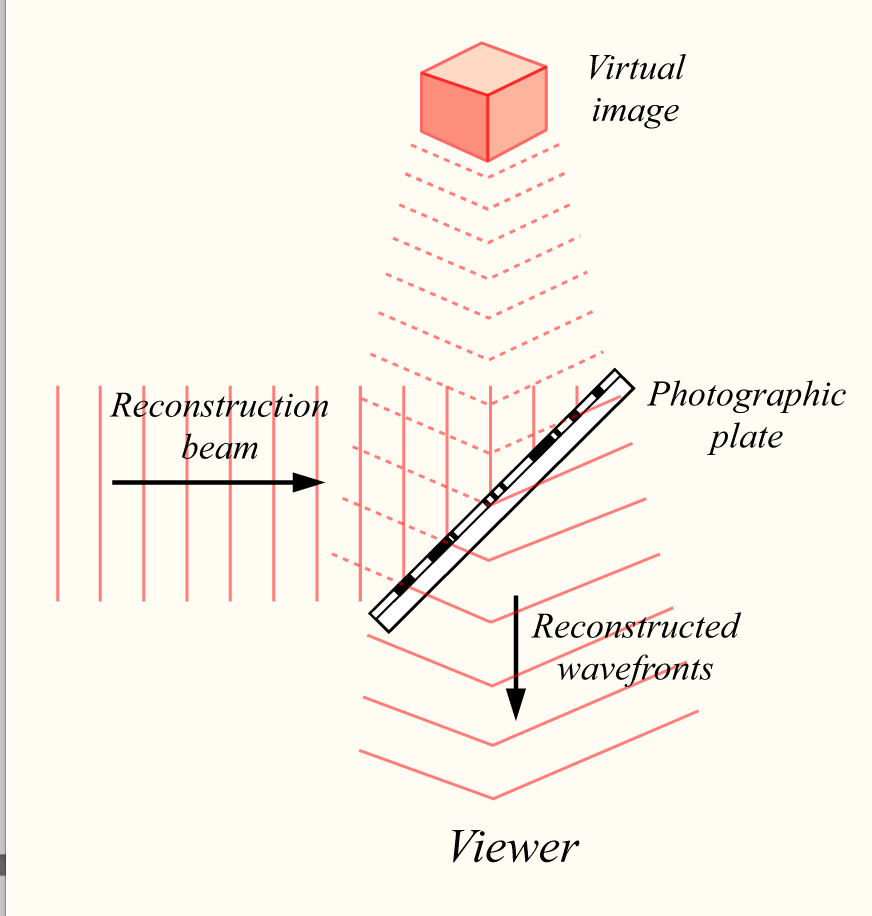
\includegraphics[width=\linewidth, height=45mm]{images/HoloRecon.png}
      \tiny \url{https://en.wikipedia.org/wiki/Holography}
       \end{minipage}
       
\\ \hline
}

%%%%%%%%%%%%%%%%%%%%%%%%%%%%%%%%%%%%%%%%%%%%

\subsection{Refraction}
\center
\begin{figure}[htbp]
    \begin{center}
	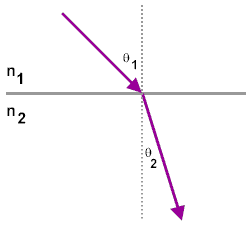
\includegraphics[width=60mm]{images/IncidentRefracted.png}
    \end{center}
    \linespread{1} 
	\caption[Incident and refracted rays]{
	\tiny http://vignette2.wikia.nocookie.net/schools/images/4/4c/097b8946-3139-4ea1-8573-05128eb66b29.gif/revision/latest?cb=20060612224020

	}
\label{IncRefRays}
\end{figure}

%%%%%%

\Table{
\hline

Index of refraction & $n \equiv \dfrac{c}{v}$

\\ \hline
}

%%%%

\Table{
\hline

I.o.R. and wavelengths

&

\MiniPg{.6}{
\center

$n = \dfrac{\lambda_0}{\lambda}$

Where $\lambda_0$ is the wavelength in vacuum and $\lambda$ is the wavelength in medium.
}
 
\\ \hline
}

%%%%

\Table{
\hline

$n$ can be $<1$ if & the phase velocity is greater than c.

\\ \hline

Snell's law & $n_i \sin \theta_i = n_f \sin \theta_f$ 

\\ \hline
}

\Table{
\hline

Draw with $n_2 > n_1$ and $n_1 > n_2$    & \begin{minipage}{.4\textwidth}
      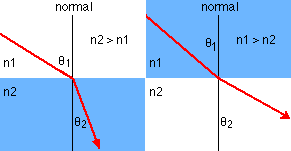
\includegraphics[width=\linewidth, height=30mm]{images/optic-snell.png}
      \tiny \url{http://www.astrosurf.com/luxorion/Physique/optic-snell.gif}
    \end{minipage}

\\ \hline
}

%%%%

\Table{
\hline

Condition for total internal reflection & $\dfrac{n_i \sin \theta_i}{n_f} > 1$

\\ \hline

Critical angle & $\theta_c = \theta_i = \arcsin \BigP{\dfrac{n_2}{n_1}}$

\\ \hline
}

%%%%

\Table{
\hline

Dispersion and general trend & $n(\lambda)$, as $\lambda \Uparrow, n \downarrow$

\\ \hline
}

%%%%

\Table{
\hline

Fraction of light reflected $R$ & $R = \Big( \dfrac{n_1 - n_2}{n_1 + n_2} \Big)^2$

\\ \hline

Fraction of light transmitted & $T = 1 - R = \dfrac{4 n_1 n_2}{(n_1 - n_2)^2 }$


\\ \hline
}

%%%%%%%%%%%%%%%%%%%%%%%%%%%%%%%%%%%%%%%

\subsubsection{Thin Films}
\Table{
\hline
\begin{minipage}{.3\textwidth}
Soap/oil film constructive and destructive interference
\end{minipage}

&

\MiniPg{.6}{

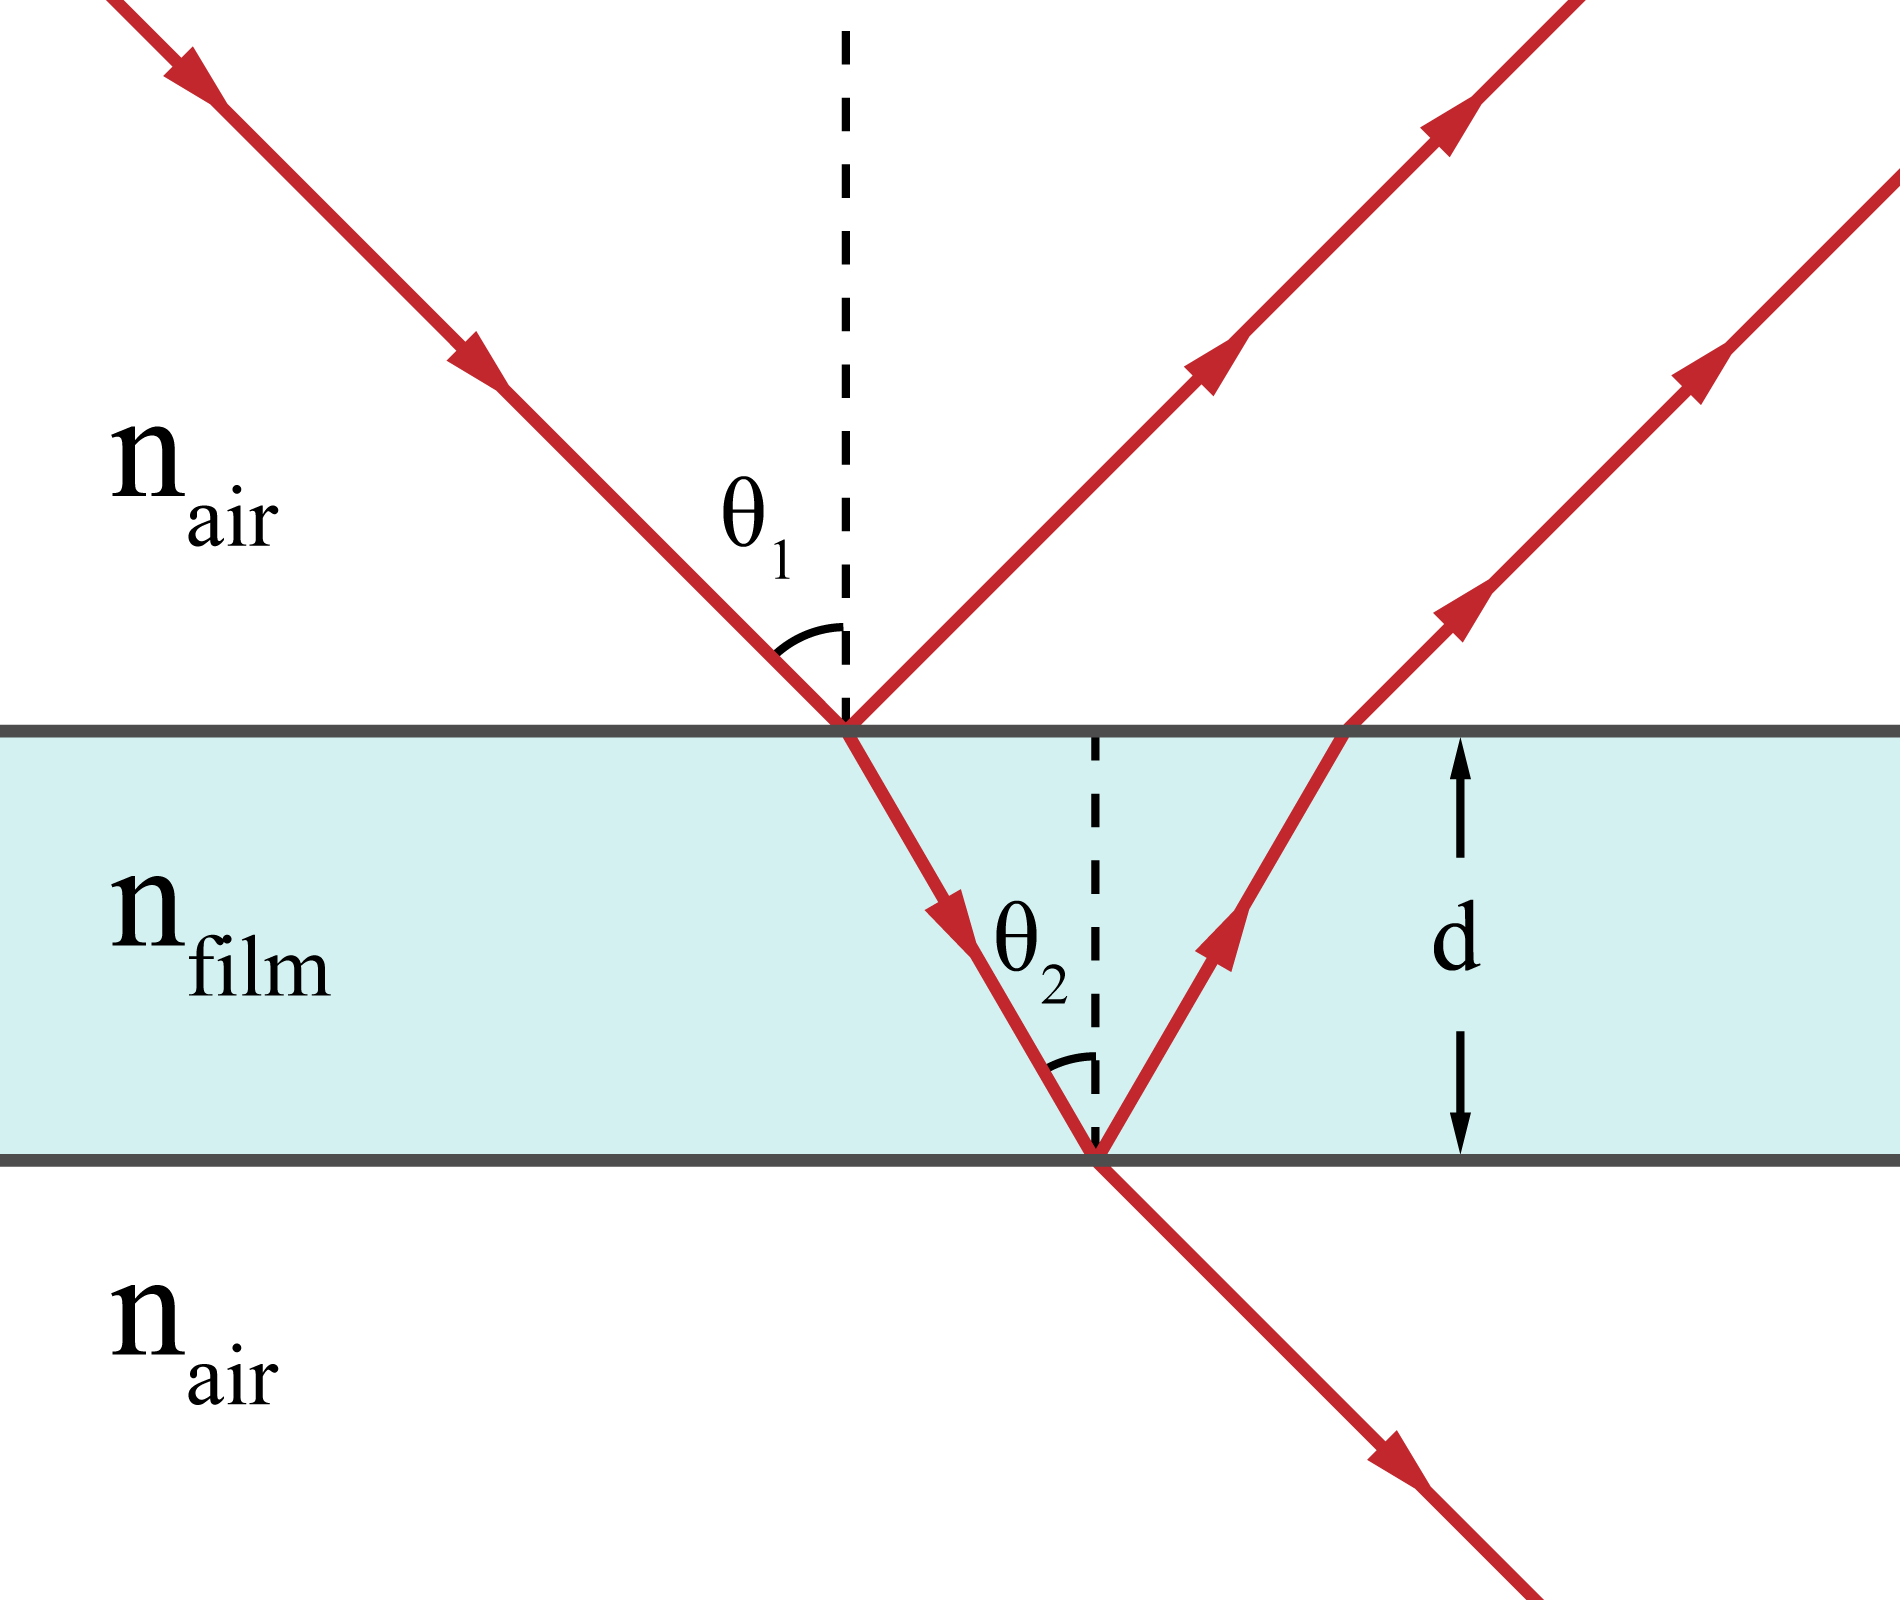
\includegraphics[width=55mm, height=40mm]{images/ThinFilmSoap.png}
      \tiny \url{https://en.wikipedia.org/wiki/Thin-film_interference}
      
      \large
      $n_{film} > n_{air}$. Also, the bottom air can be swapped with a water section, in which case $n_{film} > n_{water} >  n_{air}$, and the following equations still hold.
      
      Constructive: $2n_{film}d \cos(\theta_2) = (m-\frac{1}{2}) \lambda$
      
      Destructive: $2n_{film}d \cos(\theta_2) = m \lambda$
      

}
\\ \hline
}

%%%%

\Table{
\hline

\begin{minipage}{.3\textwidth}
Coating film constructive and destructive interference
\end{minipage}

&

\begin{minipage}{.6\textwidth}

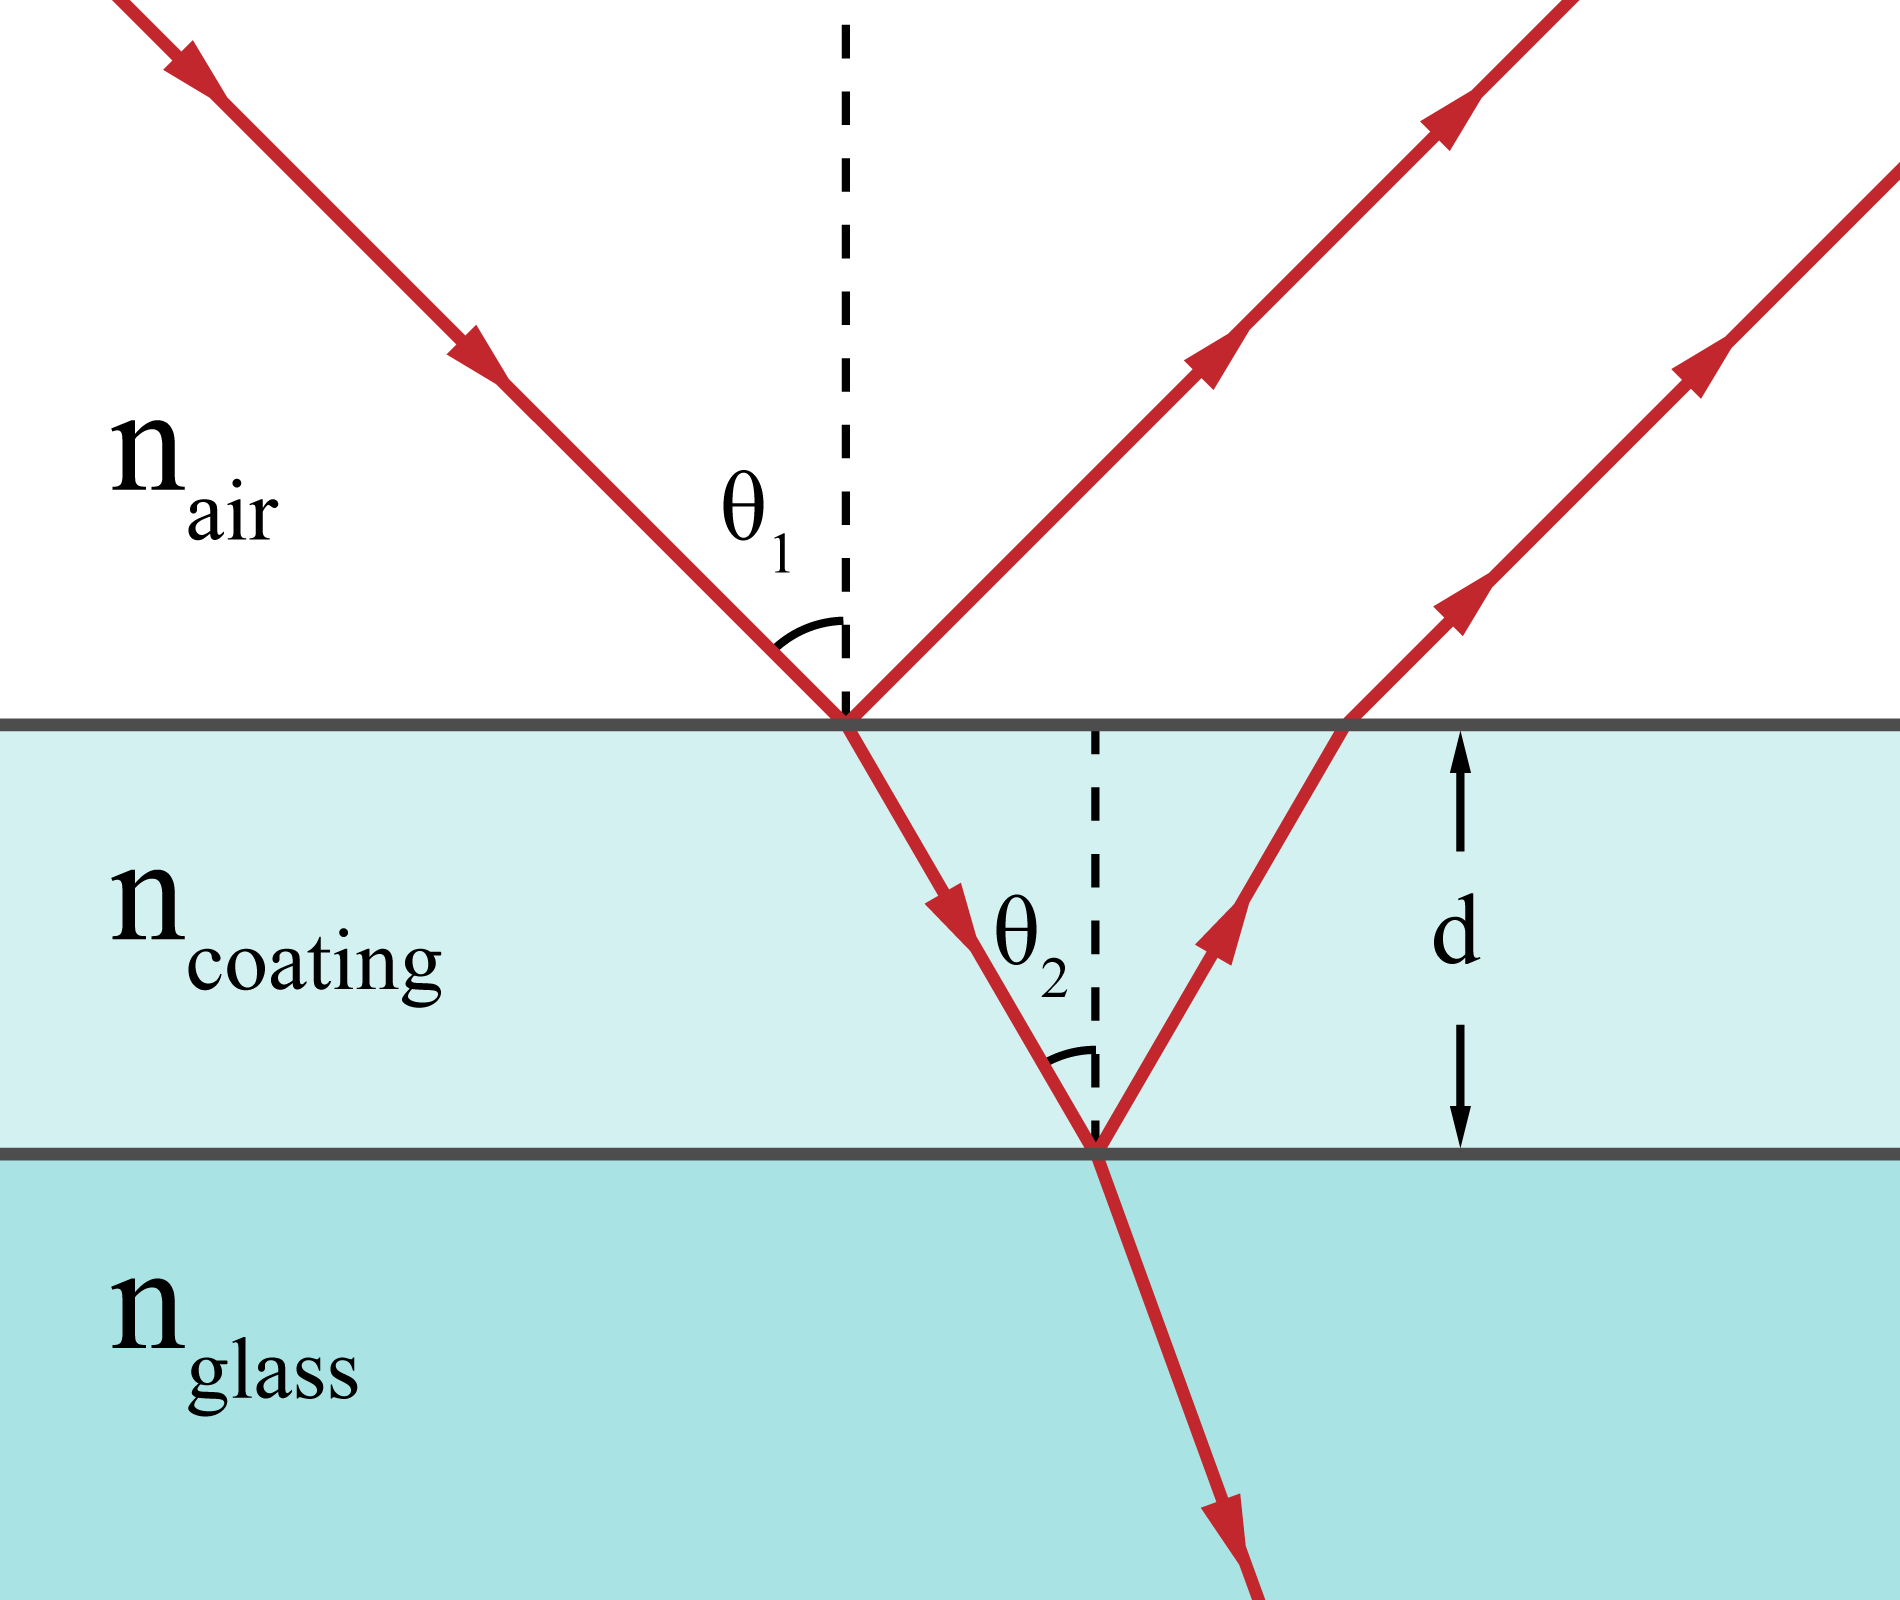
\includegraphics[width=55mm, height=40mm]{images/ThinFilmCoating.png}
      \tiny \url{https://en.wikipedia.org/wiki/Thin-film_interference}
      
      \large
      $n_{glass} > n_{film} >  n_{air}$
      
      Constructive: $2n_{coating}d \cos(\theta_2) = m \lambda$
      
      Destructive: $2n_{coating}d \cos(\theta_2) = (m-\frac{1}{2}) \lambda$
      
      
\end{minipage}

\\ \hline
}

\subsection{Diffraction}
\Table{
\hline

Single slit diffraction
&

\MiniPg{.7}{
\GraphicWHN{.55}{.4}{SingleSlit.png}
Fraunhofer Single Slit
\center
\tiny  \url{http://hyperphysics.phy-astr.gsu.edu/hbase/phyopt/imgpho/sinslit.gif}

}
 \\ \hline
}

\Table{
\hline

Double slit interference
&

\MiniPg{.7}{
\GraphicWHN{.8}{.5}{DoubleSlit.png}
\center
\tiny  \url{http://hyperphysics.phy-astr.gsu.edu/hbase/phyopt/imgpho/doubsli.gif}

\large 

}
 \\ \hline 
}

%%%%

\Table{
\hline

Diffraction grating
&

\MiniPg{.7}{
\GraphicWHN{.8}{.55}{Diffraction.png}
\center
\tiny  \url{http://hyperphysics.phy-astr.gsu.edu/hbase/phyopt/grating.html}

\large 

}

\\ \hline
}

%%%%

\Table{
\hline

Circular Aperture diffraction

&

\MiniPg{.7}{
\center

\GraphicWHN{.8}{.5}{ApertureDiff.png}
\center

Use for resolving power of telescopes.

\tiny \url{http://hyperphysics.phy-astr.gsu.edu/hbase/phyopt/cirapp2.html}

}

 \\ \hline 
}


%%%%%%%%%%%%%%%%%%%%%

\subsection{Geometrical  Optics}
\Table{
\hline

Optical Path Length & $OPL = \int_a^bn(s)\,ds$

\\ \hline
}

%%%%



%%%%%%%%%%%%


\subsubsection{Mirrors}

\center
\begin{tabular}{|p{5cm}|p{10cm}|}
\hline

For concave and convex spherical mirrors, the focal
length is & ... half the
radius of curvature of the mirror

\\ \hline
\end{tabular}

%%%%

\Table{
\hline
\MiniPg{.4}{
Spherical mirror eqn.
}

&

 \MiniPg{.6}{\center
$\dfrac{1}{f} = \dfrac{1}{d_O} + \dfrac{1}{d_i}$
}

\\ \hline

Spherical magnification & $M = \dfrac{h_i}{h_O} = -\dfrac{d_i}{d_O}$

 \\ \hline
}

%%%%

\Table{
\hline
 
 $d_O$ and object real/virtual & $d_O > 0 \rightarrow$ object in front (real). \\
 						& object in back (virtual) $\leftarrow d_O < 0$

\\ \hline
}

%%%%

\Table{
\hline

$d_i$ and image real/virtual & $d_i > 0 \rightarrow$ image in \textbf{front} (real). \\
 						& image in \textbf{back} (virtual) $\leftarrow d_i < 0$

\\ \hline
}

%%%%

\Table{
\hline

$f$ and concavexity & $f > 0 \rightarrow$ concave.convex $\leftarrow f<0$

\\ \hline

Magnification  image orientation & $M > 0 \rightarrow$ upright.inverted $\leftarrow M < 0$

\\ \hline
}


%%%%%%%%%%%%%%%%%%%%

\subsubsection{Lenses}

\Table{
\hline

\MiniPg{.3}{
Converging lens \_ mirror 

Relations for real, virtual, larger, smaller 
}
&
\MiniPg{.7}{
\center

 \begin{minipage}{.42\textwidth}
      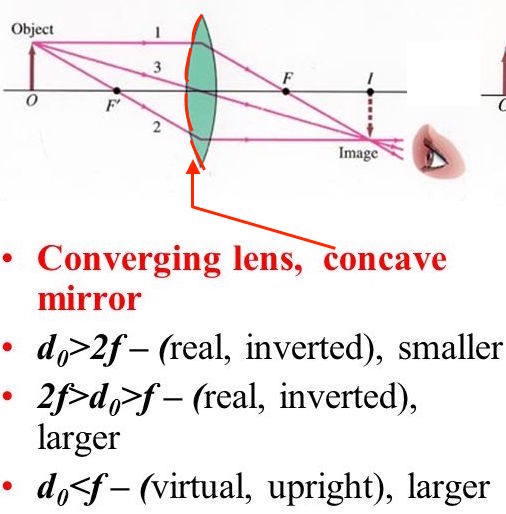
\includegraphics[width=\linewidth, height=50mm]{images/ConvLens.jpg}
       \end{minipage} 
} 

\\ \hline
}

%%%%

\Table{
\hline

\MiniPg{.3}{
Diverging lens \_ mirror 

Relations for real, virtual, larger, smaller 
}
&
\MiniPg{.7}{
\center

 \begin{minipage}{.42\textwidth}
      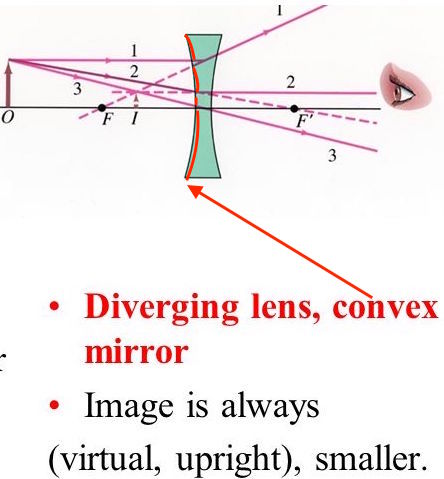
\includegraphics[width=\linewidth, height=50mm]{images/DivLens.jpg}
       \end{minipage} 
       
       \tiny \url{http://images.slideplayer.com/13/3858792/slides/slide\_13.jpg}
} 

\\ \hline

}

%%%%

\Table{
\hline

f-number or relative aperture & $\textrm{f-number} = N = \dfrac{f}{D} $ \\ 
					& where $f$ if focal length, $D$ is diameter
\\ \hline

Increased f & increased light-gathering power.

\\ \hline
}

%%%%

\Table{
\hline

Numerical aperture & $\textrm{n.a.} = n \sin \alpha$ \\

\begin{minipage}{.25\textwidth}
      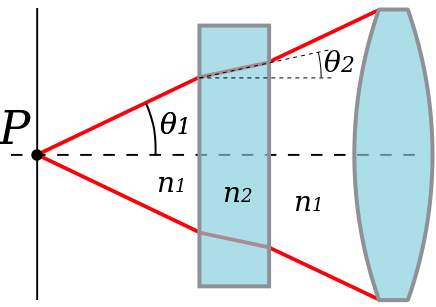
\includegraphics[width=\linewidth, height=32mm]{images/Numerical_aperture.png}
    \end{minipage} & \\
    \tiny https://en.wikipedia.org/wiki/Numerical\_aperture
     \large
    & 
    
    $\textrm{NA} = n_1 \sin \theta_1 = n_2 \sin \theta_2 $

\\ \hline
}

%%%%

\Table{
\hline

Relate NA to N (i.e. f-num) & \begin{minipage}{.25\textwidth}
      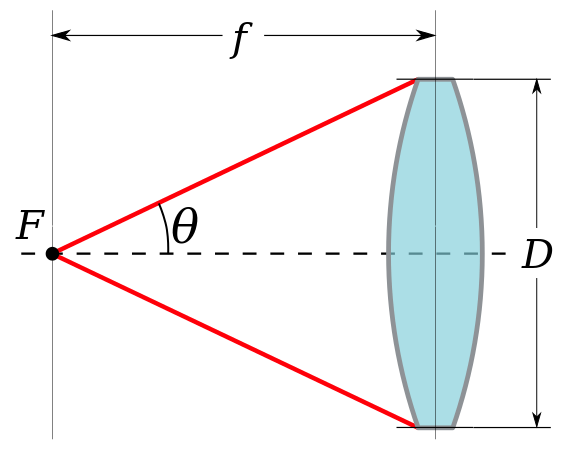
\includegraphics[width=\linewidth, height=30mm]{images/NA_fNum.png}
    \end{minipage} \\
    
     & $\textrm{NA}_i = n \sin \theta = n \sin [ \arctan \Big( \dfrac{D}{2f} \Big) ] \approx \dfrac{nD}{2f} $\\
     
      & $\Rightarrow N \approx \dfrac{1}{2 \textrm{NA}_i}$ assuming $n=1$.


\\ \hline
}

%%%%

\Table{
\hline

Formula for focal length (spherical) & $\dfrac{1}{f} = (n-1)\Big(\dfrac{1}{R_1} - \dfrac{1}{R_2} \Big),$ \\ 
& where $R_1$ is the radius of curvature for the lens \\
& nearest the object and $R_2$ is the r.o.c. for the farther

\\ \hline
}

%%%%

\Table{
\hline
\MiniPg{.4}{
Thin lens equation  (a.k.a. 'Lensmaker's formula') }

&

\MiniPg{.6}{\center
$\dfrac{1}{f} = \dfrac{1}{d_O} + \dfrac{1}{d_i}$
}

 \\ \hline
 
 $d_O$ and object real/virtual & $d_O > 0 \rightarrow$ object in front (real). \\
 						& object in back (virtual) $\leftarrow d_O < 0$

\\ \hline
}

%%%%

\Table{
\hline

$d_i$ and image real/virtual 
&

\MiniPg{.7}{\center
 $d_i > 0 \rightarrow$ image in \textbf{back} (real). 
 
 image in \textbf{front} (virtual) $\leftarrow d_i < 0$
 }
						
\\ \hline
}

%%%%

\Table{
\hline

$R_n$ and center of lens & $R_n > 0$ if center of lens in back \\
 						& $R_n < 0 $ if center of lens in front

\\ \hline
}

%%%%

\Table{
\hline

$f$ and concavexity & $f > 0 \rightarrow$ concave.convex $\leftarrow f<0$

\\ \hline

resulting $f$ for two close lenses & $\dfrac{1}{f} = \dfrac{1}{f_1} + \dfrac{1}{f_2}$

\\ \hline
}

%%%%

\Table{
\hline

Magnification & 

\MiniPg{.6}{
\GraphicWHN{.9}{.3}{LensMag.png}
\center
\tiny \url{http://hyperphysics.phy-astr.gsu.edu/hbase/geoopt/lensdet.html}
}

\\ \hline
}

%%%%

\Table{
\hline
\MiniPg{.3}{
Angular magnification of a telescope
}

&

\MiniPg{.7}{
\center
Astronomical telescope
\GraphicWHN{.85}{.3}{TelescopeAstro.png}

\center Galilean telescope
\GraphicWHN{.85}{.3}{TelescopeGali.png}
\center
For both: $M = -f_o/f_e$

}


\\ \hline
}


%%%%%%%%%%%%%%%%%%%%%%%%%%%%%%%%%%%%%%%%%%%


\subsection{Polarization}
\Table{
\hline

Malus' law & \begin{minipage}{.5\textwidth}
 First, consider electric field vector
 

$I_{transmitted} = I_0 \cos^2\theta_i$
\end{minipage}

\\ \hline

Intensity of polarized from unpolarized &  $I = I_0 \int_0^\pi \cos^2 \theta \, d \theta = \dfrac{I_0}{2}$

\\ \hline
}

%%%%

\Table{
\hline

Brewster's Angle 

&

\begin{minipage}{.7\textwidth}
\center

First, read Ch. 9 of Griffith's $EM$. It falls out of the Fresnel equations that there is 0 reflectance when

$\theta_1 + \theta_2 = 90^\circ$

Use Snell's law:

$n_1 \sin \theta_1 = n_2 \sin \theta_2$.

Let $\theta_B$ be the Brewster angle

$n_1 \sin \theta_B = n_2 \sin (90^\circ - \theta_B) = n_2 \cos \theta_B$,

Finally, $\boxed{\theta_B = \arctan\Big(\dfrac{n_2}{n_1}\Big)}$
 

\end{minipage}

\\ \hline
}

\Table{
\hline

Wire grid polarizer &  \begin{minipage}{.5\textwidth}
      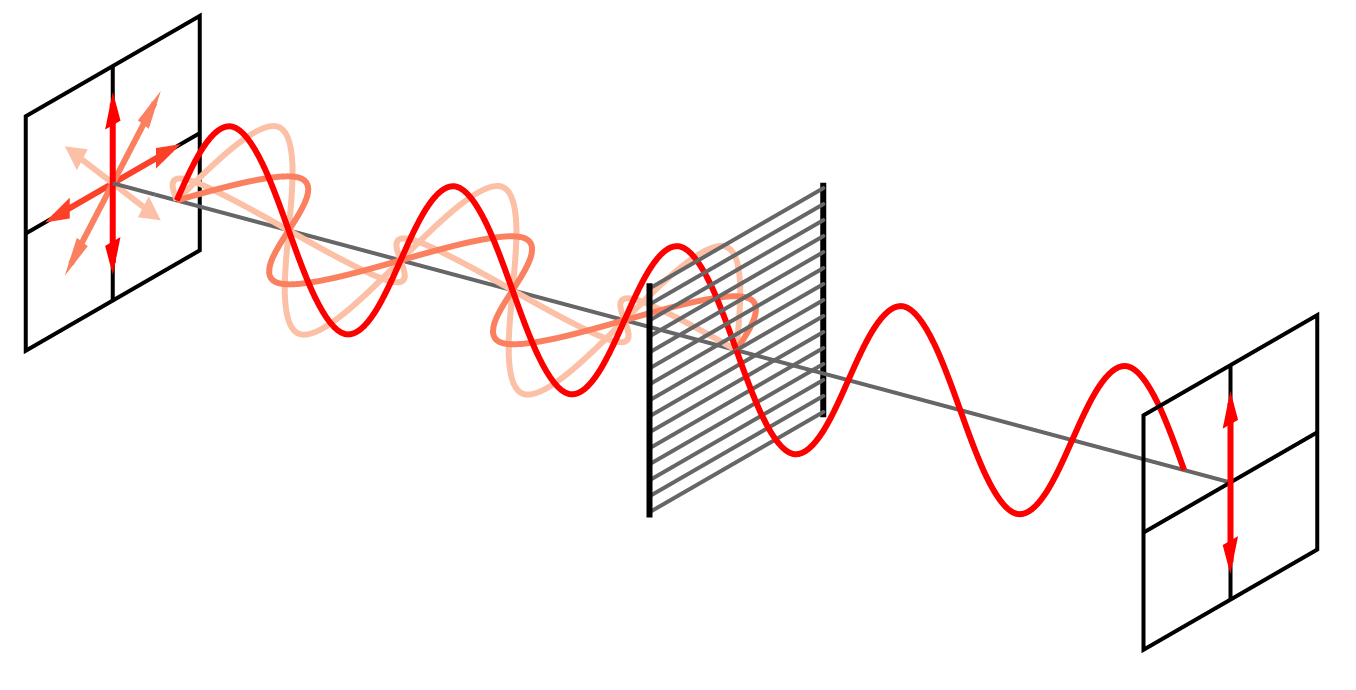
\includegraphics[width=\linewidth, height=45mm]{images/WireGridPolarizer.png}
      \tiny \url{https://en.wikipedia.org/wiki/Polarizer}
       \end{minipage}

\\ \hline
}

%%%%

\Table{
\hline

Polarized Sunglasses & \begin{minipage}{.5\textwidth}
      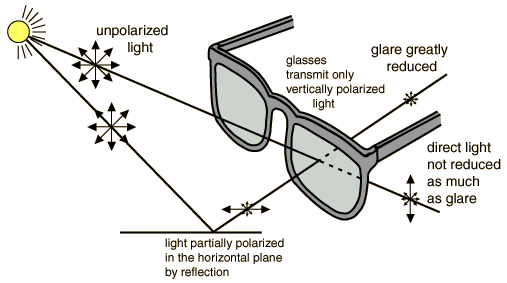
\includegraphics[width=\linewidth, height=45mm]{images/PolarizedSunglasses.png}
       \tiny \url{http://assets.openstudy.com/updates/attachments/4f175a76e4b0aeb795f5672a-jamesj-1326931194153-sunglass.gif}
       \end{minipage}
       
\\ \hline
}

%%%%

\Table{
\hline

$s$ and $p$ polarization & \begin{minipage}{.5\textwidth}
      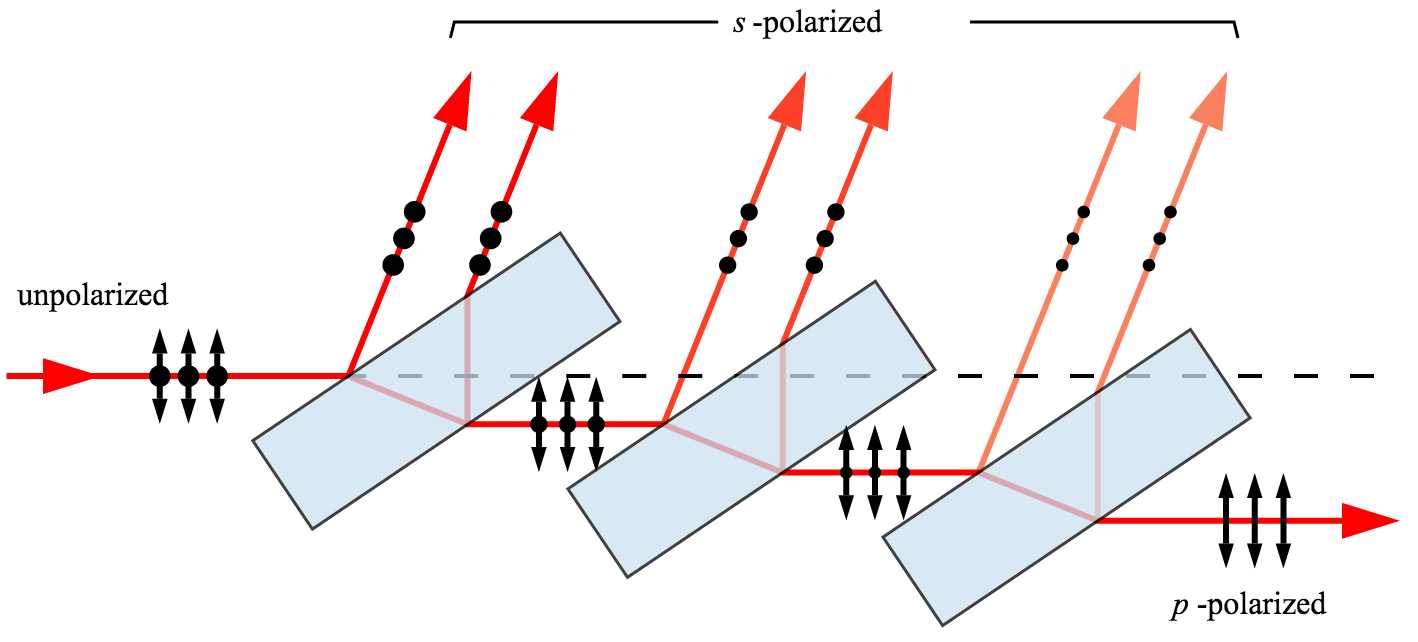
\includegraphics[width=\linewidth, height=35mm]{images/SandPpolarization.png}
      \tiny \url{https://en.wikipedia.org/wiki/Polarizer}
      
      \large Think `s' for ``smooth'' and `p' for ``pointy'' or ``points in.''
       \end{minipage}

\\ \hline
}

%%%%%%%%%%%%%%%%%%%%%%%%%%%%%%%%

\subsection{Doppler effect}
\Table{
\hline

Derivation 
Wavelengths& $c = $ velocity of waves in medium, \\
and & $v_s = $ velocity of source relative to medium, \\
Frequencies & $v_o = $ velocity of observer relative to medium. \\
& Waves travel from source to observer \\
& in the positive whatever direction: \\
& O....source)))))waves)))))observer......$>$+x \\
& Observer moving, source still: $c + v_o = \dfrac{\lambda_s}{T} $ \\
& Source moving, observer still: $c - v_s = \dfrac{\lambda_o}{T} $ \\
& $T = \dfrac{\lambda_o}{c - v_s} = \dfrac{\lambda_s}{c + v_o} $ \\
& \framebox{$\lambda_o = \dfrac{c - v_s}{c + v_o} \lambda_s$} \\
& \framebox{$f_o = \dfrac{c + v_o}{c - v_s} f_s $}

 \\ \hline
 }





\section{Thermodynamics and Statistical Mechanics}
(such as the laws of thermodynamics, thermodynamic
processes, equations of state,
ideal gases, kinetic theory, ensembles,
statistical concepts and calculation of
thermodynamic quantities, thermal
expansion and heat transfer)

\subsection{Laws of Thermodynamics}
\center
\begin{tabular}{|c|p{12 cm}|}
\hline

Zeroth Law & If two systems are in thermal equilibrium independently with a third system, they must be in thermal equilibrium with each other. This law helps define the notion of temperature.
 
\\ \hline

First Law & When energy passes, as work, as heat, or with matter, into or out from a system, its internal energy changes in accord with the law of conservation of energy. Equivalently, perpetual motion machines of the first kind are impossible.

$\Delta U = Q + W$
  
 \\ \hline
 
\end{tabular}
\flushleft

\center
\begin{tabular}{|c|p{12 cm}|}
\hline

Second Law &  In a natural thermodynamic process, the sum of the entropies of the interacting thermodynamic systems increases. Equivalently, perpetual motion machines of the second kind are impossible.
  
\\ \hline

Third Law & The entropy of a system approaches a constant value as the temperature approaches absolute zero. With the exception of non-crystalline solids (glasses) the entropy of a system at absolute zero is typically close to zero, and is equal to the logarithm of the multiplicity of the quantum ground states.
 
 \\ \hline
 
\end{tabular}
\flushleft

\center
\begin{tabular}{|c|c|}
\hline
 Fundamental Assumption & In an isolated system, all accessible microstates are equally probable.
 
 \\ \hline

\end{tabular}
\flushleft


%%%%%%%%%%%%%%%%%%%%%%%%%%%%

\subsection{Thermodynamic Processes}
\Table{
\hline

$W$ for an ideal gas & $W = - \int\limits_{V_i}^{V_f}p\,dV$

\\ \hline

$W$ in a $PV$ diagram is ... & ... area under the curve.

\\ \hline
}

%%%%

\Table{
\hline

\bf{Isothermal} & Constant temperature!

\\ \hline

$constant = $ & $PV = constant$

\\ \hline

$W = $ & $W = nRT\ln \Big[\dfrac{V_f}{V_i}\Big]$

\\ \hline

Internal energy ... & ... does not change. (Equipartition Theorem)

\\ \hline
}

%%%%

\Table{
\hline

\bf{Adiabatic} & No heat gained or lost by the system.

\\ \hline

$constant = $ & $PV^\gamma = constant$

\\ \hline

$\gamma = $ & $\dfrac{C_P}{C_V} = \dfrac{f+2}{f}$

 \\ \hline
 
 $W$ & $W =PV^\gamma \dfrac{V_f^{1-\gamma} - V_i^{1-\gamma}}{1-\gamma}$

 \\ \hline
}

%%%%

\Table{
\hline
 
 Adiabat or isotherm steeper in $PV$? & Adiabatic

\\ \hline

$W, Q, \Delta U$  for adiabatic free expansion & $W=0 \,, Q=0 \,, \Delta U = 0$

\\ \hline

Critical point & $\Big(\dfrac{\partial p}{\partial V} \Big)_T = \Big(\dfrac{\partial^2 p}{\partial V^2} \Big)_T = 0$

 \\ \hline
}

\Table{
\hline
\MiniPg{.2}{

Liquid-vapor phase diagram PV

}

&

\MiniPg{.8}{
\GraphicWHN{1}{.5}{PhasePV.png}
\tiny \url{http://cnx.org/contents/0zRIzO8t@1/13-6-Phase-Changes}
}

\\ \hline
}

%%%%

\Table{
\hline
\MiniPg{.2}{

H$_2$O phase diagram PT

}

&

\MiniPg{.8}{
\GraphicWHN{.6}{.5}{h2oPT.jpg}
\tiny \url{http://cnx.org/contents/0zRIzO8t@1/13-6-Phase-Changes}
}
\\ \hline
}

%%%%

\Table{
\hline

Fourier's law

&
\MiniPg{.7}{
\center
$\vv{q} = - k \nabla T$, where 

$\vv{q}$ is the local heat flux density, W$\cdot$m$^{-2}$,

$k$ is the material's conductivity, W$\cdot$m$^{-1}$K$^{-1}$

$\nabla T$ is the temperature gradient, K$\cdot$m$^{-1}$.
}

\\ \hline
}

%%%%%%%%%%%%%%%%%%%%%%%%%%%%%%%%

\subsection{Thermal expansion and heat transfer} 
\Table{
\hline

Heat capacity & $C = \dfrac{Q}{\Delta T}$

 \\ \hline

Specific heat capcacity & $c = \dfrac{C}{m} \rightarrow Q = mc \Delta T$
 
 \\ \hline

Latent heat & $L = Q/m$

 \\ \hline
}

%%%%%%%%%%%%%%%%%%%%%%%%%%%%%%%%%%%%%%%%%%%



\subsection{Engines \& Refrigerators}
\Table{
\hline

CW and CCW & Engines: CW. Fridges: CCW. \\
			& Think at const. $V$ what happens, $P \uparrow \downarrow$?

\\ \hline
}

%%%%

\Table{
\hline

Engine efficiency & $\eta = \dfrac{W}{Q_H} = 1 - \dfrac{Q_C}{Q_H} $

\\ \hline

Refrigerator Coefficient of performance & $\textrm{CP}_R = \eta_R = \dfrac{Q_C}{W} = \dfrac{Q_C}{Q_H - Q_C} $ 

\\ \hline

Heat pump efficiency & $\textrm{CP}_H = \eta_H = \dfrac{Q_H}{W} = \dfrac{Q_H}{Q_H - Q_C} $

\\ \hline
}

%%%%

\Table{
\hline

Carnot cycle is ... & Adiabat, Isotherm, Adiabat, Isotherm

\\ \hline

Carnot entropy & $dS = \dfrac{dQ}{T} = 0$ (Carnot)

\\ \hline
}

%%%%

\Table{
\hline

Heat entering system along isotherm & $Q = nRT\ln\Big(\dfrac{V_{end}}{V_{start}} \Big)$

\\ \hline
}

%%%%

\Table{
\hline

Carnot engine efficiency & $\eta = 1-\dfrac{T_C}{T_H}$ (Carnot)

\\ \hline

Carnot refrigerator efficiency & $ \textrm{CP}_R = \eta_R  = \dfrac{T_C}{T_H - T_C} $ (Carnot)

\\ \hline

Heat pump efficiency & $\textrm{CP}_H = \eta_H =  \dfrac{T_H}{T_H - T_C} $ (Carnot)

\\ \hline
}


%%%%%%%%%%%%%%%%%%%%%%%%%%%%%%%%%%%%%%



\subsection{Equations of state} 
\Table{
\hline

Thermodynamic identity & $dU = T\,dS- p\,dV + \mu\,dN$

\\ \hline

Change in entropy & $\Delta S \geq \frac{Q}{T}$, const. $T$, no spontaneous $\Delta S$

\\ \hline
}

%%%%

\Table{
\hline

Helmholtz Free Energy & $F = U - TS$ @ const. $T$ \\
				& $F_{sys} = $ min when $S_{universe} = $ max.

\\ \hline

Gibb's Free Energy & $G = U - TS + PV$

\\ \hline
}

%%%%

\Table{
\hline

Definition of Entropy & $S = k \ln \Omega$

\\ \hline

Definition of Temperature & $\dfrac{1}{T} = \Big( \dfrac{\partial S}{\partial U} \Big)_{V,N} $

\\ \hline
}

%%%%

\Table{
\hline

Chemical potential & $\mu = -T \Big(\dfrac{\partial S}{\partial N}\Big)_{U,V}$ \\
			& also $\mu = \Big(\dfrac{\partial U}{\partial N}\Big)_{S,V}$ \\
			& also $\mu = \Big(\dfrac{\partial F}{\partial N}\Big)_{T,V}$

\\ \hline
}

%%%%

\Table{
\hline

For systems $A$ and $B$ in diffusive contact & $A \rightarrow B$ \\ 
with $\mu_A > \mu_B$, which way do particles flow? &

\\ \hline
}

%%%%

\Table{
\hline

Heat capacity, constant volume

&

$C_V = \BigP{\dfrac{\partial E}{\partial T}}_V$

\\ \hline

Heat capacity, constant pressure

&

$C_P = \BigP{\dfrac{d E}{d T}}_P + P\BigP{\dfrac{d V}{dT}}_P$

\\ \hline
}

%%%%%%%%%%%%%%%%%%%%%%%%%%%%%%%%


\subsection{Ideal gases} 
\Table{
\hline

Ideal gas law & $PV=nRT=NkT$

\\ \hline

Relation between &  $nR$ is the number of moles times the Gas Constant.\\
 $n,N,k$ and $R$ & $Nk$ is the number of molecules times the Boltzmann Constant.
 
 \\ \hline
}

%%%%

\Table{
\hline
 
 $k=$ & $1.38 \times 10^{-23} \textrm{ J/K}$
 
 \\ \hline
 
 $R = $ & $k N_A = 1.38 \times 10^{-23} \textrm{ J/K} \, \times \, 
 6.02 \times 10^{23} \textrm{ mol}^{-1} = 8.31 \textrm{ J mol$^{-1}$ K$^{-1}$ }$
 
 \\ \hline
}

%%%%

\Table{
\hline
 
 Multiplicity of an IG & $\Omega(N,V,U) = f(N)\,V^N\,U^{fN/2}$ 
 
 \\ \hline
}

%%%%

\Table{
\hline

\MiniPg{.4}{Standard Temperature and Pressure}

&

\MiniPg{.6}{
\center
Standard Temperature = $0^{\circ} $ C $ = 273.15 $ K

Standard Pressure $1 $ Atm $= 101.3$ kPa.

1 mole of gas occupies 22.4 L.

}

\\ \hline
}


%%%%%%%%%%%%%%%%%%%%%%%%%%%%%%


\subsection{Kinetic theory} 
\Table{
\hline

Equipartition Theorem & $U = \dfrac{f}{2}NkT$

\\ \hline

$v_{rms} $ & $= \sqrt{\bar v^2} = \sqrt{\dfrac{v_1^2 + v^2_2 + ... + v^2_N}{N}}$

\\ \hline

$\dfrac{1}{2}m \bar v^2 =$ & $ \dfrac{3}{2}kT$

\\ \hline
}

%%%%

\Table{
\hline

Mean free path & $l = \dfrac{1}{n \sigma}$ where $n$ is number density $\dfrac{N}{V}$.

\\ \hline

$L_{rms} $&  $\sqrt{N}\,l$

 \\ \hline
 
 Distance between particles & $d = \Big( \dfrac{V}{N} \Big)^{1/3}$
 
 
\\ \hline
}

%%%%

\Table{
\hline
Degrees of freedom

&
\begin{minipage}{.75\textwidth}

      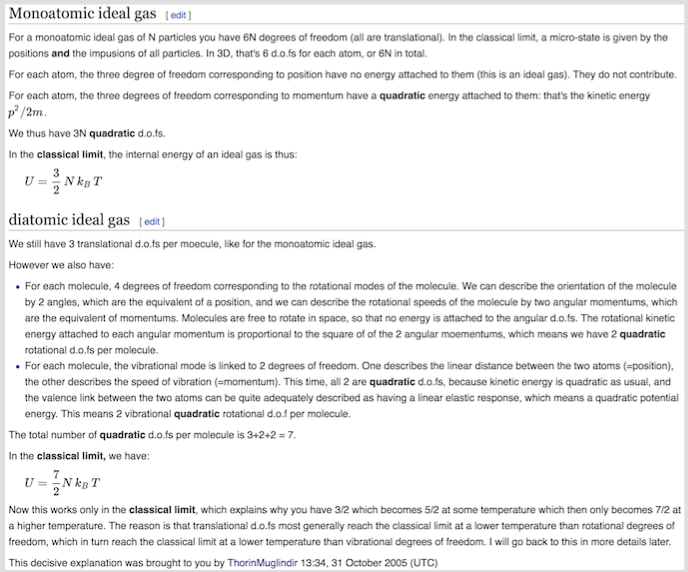
\includegraphics[width=\linewidth, height=130mm]{images/DOFs.png}

\tiny \url{https://en.wikipedia.org/wiki/Talk\%3ADegrees_of_freedom_(physics_and_chemistry)}

\tiny \url{http://demonstrations.wolfram.com/TheSixDegreesOfFreedomOfADiatomicMolecule/}
\end{minipage}

\\ \hline
}


%%%%%%%%%%%%%%%%%%%%%%%%%%%%%%%%%%%%%


\subsection{Ensembles} 
\Table{
\hline

Fermi energy & 
\begin{minipage}{.7\textwidth}
the energy difference between the highest and lowest occupied single-particle states in a quantum system of non-interacting fermions at absolute zero temperature
\end{minipage}

\\ \hline
}

%%%%

\Table{
\hline

\begin{minipage}{.3\textwidth}
Fermi Energy of infinite square well with N atoms
\end{minipage}
&
\begin{minipage}{.7\textwidth}
$E_F = \dfrac{\hbar^2 \pi^2}{2 m L^2}(N/2)^2$ for even $N$, and for odd $N$ substitue $N-1$ for $N$ in the expression.
\end{minipage}

\\ \hline
}

%%%%

\Table{
\hline

\begin{minipage}{.3\textwidth}
Fermi energy of a metal with $N$ electrons per volume $V$
\end{minipage}
&
\begin{minipage}{.7\textwidth}
\center
Metal $\approx$ 3-D ISW

$E_{n_x,n_y,n_z} = E_0 + \dfrac{\hbar^2 \pi^2}{2mL^2}(n_x^2 + n_y^2 + n_z^2)$,

but let $\vv{n} = \{n_x,n_y,n_z\}$ so that

$E_{\vv{n}} = E_0 + \dfrac{\hbar^2 \pi^2}{2mL^2}|\vv{n}|^2$.

In the ground state, the number of fermions is

$N = 2 \times \dfrac{1}{8} \times \dfrac{4}{3}\pi n_F^3$ where $|n_F|$ is the radius of the Fermi-sphere in $n$-space. Thus,

$n_F = \Big(\dfrac{3N}{\pi}\Big)^{1/3}$.

So, the Fermi energy is

$E_F = \dfrac{\hbar^2 \pi^2}{2mL^2}n_F^2 = \dfrac{\hbar^2 \pi^2}{2mL^2}\Big(\dfrac{3N}{\pi}\Big)^{2/3}$

$\boxed{E_F = \dfrac{\hbar^2}{2m}\Big(\dfrac{3\pi^2N}{V}\Big)^{2/3} }$

\end{minipage}

\\ \hline
}

%%%%

\Table{
\hline

\begin{minipage}{.3\textwidth}
Fermi temperature, momentum, velocity and wave vector
\end{minipage}
 &
\begin{minipage}{.7\textwidth} 
  $T_F = \dfrac{E_F}{k_B}$; \; \; \;  $p_F = \sqrt{2m_eE_F}$; \; \; \; $v_F = \dfrac{p_F}{m_e}$; \; \; \; $k_F = \dfrac{p_F}{\hbar}$
\end{minipage}

\\ \hline

typical Fermi energy for metal & $10^{28}$ to  $10^{29}$ e/m$^3$ $\rightarrow E_F \approx 2 $ to $ 10$ eV

\\ \hline
}


%%%%
\Table{
\hline

\begin{minipage}{.3\textwidth}
Number of independent oscillators in crystal with $N$ atoms 
\end{minipage}
& $3N$ according to Einstein and Debye

\\ \hline
}

%%%%

\Table{
\hline

Multiplicity of an Einstein Solid & $\Omega = {{q+N-1}\choose{q}} = \dfrac{(q+N-1)!}{q!\, (1 +N-1 - q)!}$ \\

& $ = \dfrac{(q+N-1)(q + N - 2) ... (q + N - q) (N - 1) (N-2) ...}{q!  (N - 1) (N-2) ...}$ \\

& $ = \dfrac{(q+N-1)(q + N - 2) ... N}{q!}$

\\ \hline
}

%%%%

\Table{
\hline

Entropy of an Einstein Solid & $S = k (\ln (1 + N)! - \ln q! - \ln N!)$ \\
 & Stirling's $\rightarrow$ \\
 & $\ln \Omega \approx (q + N) \ln(q + N) - (q+ N) - q \ln q + q - N \ln N + N$ \\
 & $=(q+N) \ln(q + N) - q \ln q - N \ln N $ \\
 & ... and ...\\
 & $\ln(q + N) = \ln \Big[q\Big(1 + \dfrac{N}{q} \Big) \Big]$ \\
 & $ = \ln q + \ln \Big( 1 + \dfrac{N}{q} \Big)$ \\ 
 & $ \approx \ln q + \dfrac{N}{q}$  assuming $q>>N$\\
 & ... algebra ... \\
 & $S = k \ln \Omega = k \Big( N \ln \dfrac{q}{N} + N + \dfrac{N^2}{q}\Big) $ \\
 & drop the last term \\
 & $S \approx Nk\Big(\ln \dfrac{q}{N} + 1\Big)$ \\
 & if energy unit $hf = \epsilon$ and tot. int. energy $U = q \epsilon$ then \\
 & \framebox{$S = Nk\Big(\ln \dfrac{U}{ q \epsilon} + 1)$}
 
 \\ \hline
}

%%%%

\Table{
\hline

Temperature Einstein Solid & $T = \Big(\dfrac{\partial S}{\partial U} \Big)^{-1} = \dfrac{U}{Nk}$

\\ \hline

Energy of an Einstein Solid & $U = NkT$
\\ \hline
}


%%%%%%%%%%%%%%%%%%%%%%%%%%%%%%%


\subsection{Statistical concepts and calculation of thermodynamics quantities} 
\Table{
\hline

Stirling's Approximation & $\ln (N!) = N \ln (N) - N$

\\ \hline

Boltzmann Factor & Any term of the form $e^{-E / kT}$

\\ \hline
}

%%%%

\Table{
\hline

\begin{minipage}{.4\textwidth}
For a thermodynamic system with two accessible states, what is the ratio of probability that it's in state 1 to the probability that it is in state 2?
\end{minipage}
& $\dfrac{P(1)}{P(2)} =  \dfrac{e^{-E_1/kT}}{e^{- E_2/kT}}$

\\ \hline
}

%%%%

\Table{
\hline

Probability of $E_i$ & $P(i) = \dfrac{e^{-E_i / kT}}{Z}$

\\ \hline

Partition function 

&

$Z = \sum_{\textrm{all $\mu$states $i$}} e^{-E_i / kT}  = \sum_{\textrm{all energies $E$}} g(E)\, e^{-E/kT}$
 
 \\ \hline
}

%%%%

\Table{
\hline
 
 Average energy & \begin{minipage}{.7\textwidth}
 
$ \braket{E} = \sum_i E_i p_i = \dfrac{\sum_i E_i e^{-E_i/k_BT}}{\sum_j e^{-E_i/k_BT}}$

Conveniently, $\braket{E} = -\dfrac{1}{Z} \dfrac{\partial Z}{\partial \beta}_{N,V}$
or
$\braket{E} = - \dfrac{\partial \ln Z}{\partial \beta}$

where $\beta \equiv \dfrac{1}{k_B T}$.
 
 \end{minipage}
 
 \\ \hline
}

%%%%

\Table{
\hline
 
 Statistical entropy & $S = k \sum_i p_i \ln p_i $ if high $T$ then $S = N k \ln Z$.
 
 \\ \hline
 
Gibbs factor system in diffusive eq. & $P(N,i) = \dfrac{1}{Z}e^{(N\mu - E_i)/kT}$ \\
and Thermal contact with reservoir & $e^{(N\mu - E_i)/kT}$ is the Gibbs factor.

\\ \hline

Thermal diffusive partition func. & $Z_{N,i} = \sum_i e^{(N\mu - E_i)/kT}$

\\ \hline
}

%%%%

\Table{
\hline

\MiniPg{.3}{
Maxwell-Boltzmann assumptions
}

&

\MiniPg{.7}{
\center

We are concerned with the number of particles in a given microstate $i$.

$\dfrac{N_i}{N} = \dfrac{e^{-E_i/ kT}}{\sum_j e^{-E_j/ kT}}$

From Wikipedia: "The assumptions of this equation are that the particles do not interact, and that they are classical; this means that each particle's state can be considered independently from the other particles' states. Additionally, the particles are assumed to be in thermal equilibrium.``

}

\\ \hline
}

%%%%

\Table{
\hline

\MiniPg{.3}{
Maxwell-Boltzmann distribution for momentum vector
}

&

\MiniPg{.7}{
\center

$\dfrac{N_i}{N} = \dfrac{1}{Z} \exp \Big[ -\dfrac{p^2_{i,x} + p^2_{i,y} + p^2_{i,z}}{2mkT} \Big]$

Probability density function for finding a molecule with a particular momentum vector:

$f_{\bold{p}} (p_x, p_y, p_z) = \dfrac{c}{Z} \exp \Big[ -\dfrac{p^2_x+ p^2_y + p^2_z}{2mkT} \Big]$.

Normalize using the Gaussian integral ( $\int_{-\infty}^{\infty} e^{-ax^2} \, dx = \sqrt{\pi/a}$ ) to find that $c = Z(2 \pi mkT)^{-3/2}.$

$\boxed{f_{\bold{p}} (p_x, p_y, p_z) = (2 \pi mkT)^{-3/2} \exp \Big[ -\dfrac{p^2_x+ p^2_y + p^2_z}{2mkT} \Big]}$

}

\\ \hline
}

%%%%

\Table{
\hline

\MiniPg{.3}{Maxwell-Boltzmann energy distribution}

&

\MiniPg{.7}{
\center
Consider $d^3 \bold{p}$ as an infinitesimal phase-space volume of momenta corresponding to the interval $dE$. Specifically, the interval $dE$ coincides with a spherical shell of thickness $d|\bold{p}|$ in momentum space. Use this and the energy-momentum dispersion relation to find

$d^3\bold{p} = 4 \pi |\bold{p}^2| d|\bold{p}| = 4 \pi m \sqrt{2mE} \, dE$

Now impose the following:

\MPalign{
f_E(E)\,dE &= f_{\bold{p}}(\bold{p}) \, d^3\bold{p} \\
 & =  (2 \pi mkT)^{-3/2} e^{-E/kT} \, 4 \pi m\sqrt{2mE} \, dE \\ 
f_E(E) & = \boxed{2 \sqrt{\dfrac{E}{\pi}} \BigP{ \dfrac{1}{kT}}^{3/2} e^{-E/kT} }

}

}

\\ \hline
}

%%%%

\Table{
\hline

\MiniPg{.3}{Maxwell-Boltzmann velocity distribution}

&

\MiniPg{.7}{
\center

Use $f_{\bold{v}} \,d^3 v = f_{\bold{p}} \BigP{ \dfrac{dp}{dv}}^3 \, d^3 v$ and $\bold{p} = m \bold{v}$ and the momentum distribution above to get

$\boxed{f_{\bold{v}} (v_x, v_y, v_z) = \BigP{\dfrac{m}{2 \pi kT}}^{3/2} \exp\Big[- \dfrac{m(v_x^2 + v_y^2 + v_z^2)}{2kT} \Big]}$.

This can be expressed as the product of three speed distributions for the three directions: $f_{\bold{v}}(v_x,v_y,v_z) = f_v(v_x) f_v(v_y) f_v(v_z)$, where

$\boxed{f_v(v_i) = \sqrt{\dfrac{m}{2 \pi kT}} \exp\Big[-\dfrac{mv_i^2}{2kT} \Big]}$

Note: $\mu_i = 0$, $\mu_{\bold{v}} = \bold{0}$, $\sigma_i = \sqrt{kT/m}$, and $\sigma_{\bold{v}} = \sqrt{3kT/m}$.

}

\\ \hline
}

%%%%%%%%%%%%%%%%%%%%%%%%%%%%%%%%

\subsection{Black-body radiation} 

\Table{
\hline

\MiniPg{.3}{
Planck's law
}

&

\MiniPg{.7}{

The spectral radiance of a body at absolute temperature $T$ is given by

$B_{\nu} ( \nu, T) = \dfrac{2h\nu^3}{c^2} \dfrac{1}{e^{\frac{h \nu}{k_B T}} - 1}$
$B_{\lambda} ( \lambda, T) = \dfrac{2hc^2}{\lambda^5} \dfrac{1}{e^{\frac{h c}{\lambda k_B T}} - 1}$

Note: $[B_{\nu}] =$ W$\cdot$sr$^{-1} \cdot $m$^{-2} \cdot $Hz$^{-1}$ and $[B_{\lambda}] =$ W$\cdot$sr$^{-1} \cdot $m$^{-3}$.

}

\\ \hline
}

%%%%

\Table{
\hline

\MiniPg{.3}{

Stefan-Boltzmann Law

}

&

\MiniPg{.7}{
Radiant exitance or emissive power, $\dfrac{P}{A}= \varepsilon \sigma (T^4 - T_C^4)$,

where $\varepsilon$ is the emissivity ($\varepsilon = 1$ for blackbody, $<1$ for `gray' body),  $\sigma \approx 5.67 \textrm{E}-8$ is the S-B constant, and $T_C$ is the temperature of cooler surroundings.
}
 
 \\ \hline
}

%%%%

\Table{
\hline

Wien's displacement law

&
\MiniPg{.6}{
The spectral radiance of black body radiation per unit wavelength, peaks at 
$\lambda_{max} = \dfrac{b}{T}$, where Wien's displacement constant $b = 2.9 \times 10^{-3} \textrm{m K}$.
}
\\ \hline
}





\section{Quantum Mechanics}
(such as fundamental concepts, solutions of
the Schrodinger equation (including
square wells, harmonic oscillators,
and hydrogenic atoms), spin, angular
momentum, wave function symmetry,
elementary perturbation theory)

\subsection{Fundamental concepts}
\subsubsection{Some Common Integrals and Probability Theory}
\Table{
\hline

$\textrm{erf}(\infty), \textrm{erf}(-\infty) $ & $\textrm{erf}(\infty) = 1, \textrm{erf}(-\infty) = -1$

\\ \hline

The Gaussian Integral & Option 1: Know the error function. \\

$\int_{-\infty}^{+\infty} e^{-ax^2}\,dx = $ & $\dfrac{\sqrt{\pi}}{2\sqrt{a}} \, \textrm{erf}(x\sqrt{a})\bigg|_{-\infty}^{+\infty} = \sqrt{\dfrac{\pi}{a}}$ \\ 

& Option 2: Use polar coordinate trick. \\
& $I^2 = \Big( \bigintss_{- \infty}^{\infty} e^{-ax^2} \, dx \Big)^2$ \\
& $ = \bigintss \bigintss_{\textrm{\textbf{R}}^2} e^{-a(x^2+y^2)} \, d(x,y) $ \\
& $ = \bigintss_0^{2 \pi} \bigintss_0^{\infty} e^{-ar^2} r \,dr\,d\theta $ \\
& $ = 2\pi \bigintss_0^{\infty} re^{-ar^2} dr $ \\
& Let $s = -ar^2$ and then $ds = -2ar \, dr$. \\
& $I^2 = \dfrac{\pi}{a} \bigintss_{-\infty}^{0} e^s \, ds $ \\
& $ = \dfrac{\pi}{a}$ \\
& $I = \sqrt{\dfrac{\pi}{a}}$ 

\\ \hline
}

%%%%%%%%%%

\Table{
\hline

$\langle f(x) \rangle = $ & $\int_{-\infty}^{+\infty} f(x)p(x)\,dx$

\\ \hline
\begin{minipage}{.3\textwidth}
$Q$ is an operator corresponding to physical observable $x$. One may obtain the expectation value of $x$ by ...
\end{minipage}
&
\begin{minipage}{.6\textwidth}
... using $\braket{Q} = \braket{\psi^*|Q|\psi} = \int\psi^*Q\psi$, from which one may obtain the expectation value of $x$ by knowing how $Q$ corresponds to $x$.
\end{minipage}

\\ \hline
}

%%%%%%%%%%


\Table{
\hline

Standard deviation &
\MiniPg{.7}{
\center
 $\sigma = \sqrt{ \braket{(\Delta x)^2} }$

$ = \sqrt{ \braket{ x^2} - \braket{ x}^2 }$

For a measurement $Q$ corresponding to hermitian operator $\hat{Q}$,

$\sigma^2 = \braket{(\hat{Q} - \braket{Q} )^2}$. % = \braket{\Psi|(\hat{Q} - q)^2 \Psi}$
}

\\ \hline

Normalize $\psi (\phi) = A e^{im \phi}$ & $1 = \int |\psi(\phi)|^2 d \, \phi  = A^2\int_0^{2 \pi} e^{im\phi}e^{-im \phi} d\,\phi = 2 \pi A^2$\\
 &$ A = \dfrac{1}{\sqrt{2 \pi}}$
 
\\ \hline
}

%%%%%%%%%%%%%%%%%%%%%%%%%%

\subsubsection{Formalism and Linear Algebra}

This section could be called 'Griffiths runs the voodoo down' because it is a list of the cardinal equations of QM as explained in Chapter 3 of, \textit{Introduction to Quantum Mechanics}.
\Table{
\hline

vector representation 
&
$\ket{\alpha} \rightarrow \bold{a} = \SmallMatrix{
a_1 \\
a_2 \\
\vdots \\
a_N 
}
$

\\ \hline

\MiniPg{.3}{
Inner product of two vectors
}
&
$\braket{\alpha | \beta} = a_1^*b_1 + a_2^*b_2 + ... a_N^*b_N.$

\\ \hline

Properties of an inner product
&
\MiniPg{.7}{
\center

$\braket{\beta|\alpha} = \braket{\alpha|\beta}^*$

$\braket{\alpha | \alpha} \geq 0$, and $\braket{\alpha | \alpha} = 0 \iff \ket{\alpha} = 0$, 

$\bra{\alpha} | (b|\ket{\beta} + c|\ket{\gamma}) = b \braket{\alpha | \beta} + c \braket{ \alpha | \gamma}$.
.
}

\\ \hline

Linear transformations

&

\MiniPg{.7}{
\center
Linear transformations $T$ are represented by matrices.

$\ket{\beta} = T \ket{\alpha} \rightarrow \bold{b} = \bold{Ta} = \SmallMatrix{
t_{1 \, 1} & t_{1 \, 2} & ... & t_{1 \, N} \\
t_{2 \, 1} & t_{2 \, 2} & ... & t_{2 \, N} \\
\vdots     & \vdots	 & .\vdots. & \vdots \\
t_{N \, 1} & t_{N \, 2} & ... & t_{N \, N} 
}\SmallMatrix{
a_1 \\
a_2  \\
\vdots \\
a_N
}
$.

}

\\ \hline
}

\Table{
\hline

Hilbert space
&
\MiniPg{.7}{

Hilbert space comprises the set of all square-integrable functions, on a specified interval, $f(x)$ such that $\bigint_a^b |f(x)|^2 dx < \infty$.

Wave functions live in Hilbert space.

}

\\ \hline

\MiniPg{.3}{
Inner product of two functions $f(x)$ and $g(x)$.
}

&

\MiniPg{.7}{

\center

$\braket{f|g} \equiv \bigint_a^b f(x)*g(x) dx$.

}

\\ \hline

Orthonormality

&

\MiniPg{.7}{
\center
A set of functions is orthonormal if they are normalized and mutually orthogonal:
$\braket{f_m|f_n} = \delta_{mn}$.
}

\\ \hline
}

%%%%

\Table{
\hline

Completeness

&

\MiniPg{.7}{
\center

A set of functions is complete if any other function (in Hilbert space) can be expressed as a linear combination of them:
$$f(x) = \sum_{n=1}^{\infty} c_n f_n(x) $$

}

\\ \hline

Coefficients

&

\MiniPg{.7}{
\center
If the functions $\{f_n(x)\}$ are orthonormal, the coefficients are $c_n = \braket{f_n|f} = \bigint f_n(x)^*f(x,t) \, dx.$

}

\\ \hline

Normalization condition

&

\MiniPg{.7}{
\center

$ \int_{-\infty}{^\infty}dx \, |\Psi(x,t)|^2 = 1$

$ \sum_n |c_n|^2 = 1$.

}

\\ \hline
}

%%%%

\Table{
\hline

Expectation value

&

\MiniPg{.7}{
\center

The expectation value of an observable $Q(x,p)$:

$\braket{Q} = \int \Psi^*\hat{Q}\Psi dx = \braket{\Psi|\hat{Q} \Psi}$

The expectation value may not be the eigenvalue (measured value) of a Hermitian operator (observable).
}

\\ \hline

\MiniPg{.3}{

Probability of getting eigenvalue $q_n$ associated with eigenfunction $f_n(x)$

}

&

\MiniPg{.7}{

Probability for discrete is $|c_n|^2$.

Probability for continuous in range $dz$ is $|c(z)|^2 dz$.

}

\\ \hline
}

%%%%

\Table{
\hline

Most probable value

&

\MiniPg{.7}{
\center
Mode not mean! Find max of $|\psi|^2$. Ex: Most probable $r$ for radially dependent, spherically symmetrical wave function $\psi(r)$.

$|\psi|^2 \, dV = |\psi|^2 4 \pi r^2 \, dr$

For max, $\dfrac{d}{dr} |\psi|^2 4 \pi r^2 = 0$. Solve for $r$ to find most probable radial coordinate.
}

\\ \hline
}

%%%%

\Table{
\hline
\MiniPg{.3}{
Hermitian operators as measurements
}

&

\MiniPg{.7}{

The outcome of a measurement is real, so we must have $\braket{Q} = \braket{Q}^*.$ Therefore, $\braket{\Psi|\hat{Q} \Psi} = \braket{\hat{Q} \Psi|\Psi}.$ \textbf{The operators representing observables are hermitian:} $\braket{f|\hat{Q} f} = \braket{\hat{Q} f | f}$ for all $f(x)$. The last expression implies $\braket{f|\hat{Q} g} = \braket{\hat{Q} f | g}$ for all $f(x)$ and $g(x)$.

}

\\ \hline
\MiniPg{.3}{
Hermitian operators as linear transformations
}

&

\MiniPg{.7}{
\center
Hermitian operators are linear transformations: $\ket{\beta} = \hat{Q} \ket{\alpha}$.

Just as vectors are represented, with respect to a particular basis $(\ket{e_n}),$ by their components,

$\ket{\alpha} = \sum_n a_n\ket{e_n},$ with $a_n = \braket{e_n|\alpha}$,

operators are represented by their matrix elements $\braket{e_m|\hat{Q}|e_n} \equiv Q_{mn}$. In this notation, the linear transformation looks like this: $\sum_n b_n \ket{e_n} = \sum_n a_n \hat{Q} \ket{e_n}$. Take the inner product with $\ket{e_m}$, i.e. $\sum_n b_n \braket{e_m|e_n} = \sum_n a_n \bra{e_m} \hat{Q} \ket{e_n}$, and hence $b_m = \sum_n Q_{mn}a_n$.

Check out this way dope list of QM operators 
\small \url{https://en.wikipedia.org/wiki/Operator_(physics)\#Table_of_QM_operators}.

}

\\ \hline
}



\Table{
\hline

braket

&

\MiniPg{.7}{
\center
Ket is a vector, but what is bra?

In function space it can be thought of as an instruction to integrate: $\bra{f} = \bigint f^* [some \, ket] dx.$

In finite-dimensional vector space, bra is a row vector: $\bra{\alpha} = (a_1^* \ \ a_2^* \ \ ... \ \ a_n^*)$
}

\\ \hline

Projection operator

&
\MiniPg{.7}{
\center
$\hat{P} \equiv \ket{\alpha}\bra{\alpha}$

$\hat{P}\ket{\beta} = \braket{\alpha|\beta} \, \ket{\alpha}.$

}

\\ \hline

Identity operator

&

\MiniPg{.7}{
\center
If $\{\ket{e_n}\}$ is a discrete orthonormal basis, then $\sum_n \ket{e_n}\bra{e_n} = 1$ (the identity operator).

$\sum_n \ket{e_n} \braket{e_n|\alpha} = \ket{\alpha}$.

For orthonormalized continuous basis, $\bigint \ket{e_z} \bra{e_z} \, dz = 1$.
}

\\ \hline

Inverse of an operator & $\hat{A}^{-1}$ such that $\hat{A}\hat{A}^{-1} = \hat{A}^{-1}\hat{A} = \hat{I}$

\\ \hline
}

%%%%

\Table{
\hline

\MiniPg{.3}{

Determinate states

}

&

\MiniPg{.7}{

Determinate states are the physical meaning of the eigenfunctions of hermitian operators. If the eigenfunction spectrum is discrete, the eigenfunctions lie in the Hilbert space and constitute physically realizable states. If the spectrum is continuous, they are non-normalizable and do not represent possible wave functions, though linear combinations of them may be normalizable.

}

\\ \hline
\MiniPg{.3}{

Properties of hermitian operators
}

&

\MiniPg{.7}{
\center
I. Their eigenvalues are real.

$\hat{Q}f = qf$

II. Eigenfunctions belonging to distinct eigenvalues are orthogonal.

If $\hat{Q}f = qf$ and $\hat{Q}g = q'g$, then $\braket{f|g} = 0$.

}

\\ \hline

\MiniPg{.3}{
Hermitian conjugate or adjoint 
}

&
\MiniPg{.7}{
$\hat{Q}^\dagger$ such that $\braket{f|\hat{Q} g} = \braket{\hat{Q}^\dagger f|g}$ for all $f$ and $g$. A Hermitian operator is equal to its hermitian conjugate: $\hat{Q}  = \hat{Q}^\dagger$. Also, $(\hat{Q}\hat{R})^\dagger = \hat{R}^\dagger \hat{Q}^\dagger$.
}



\\ \hline
}

%%%%


\Table{
\hline

Compatibility Theorem 
&
\MiniPg{.7}{
Let us have two observables,  $A$ and $B$, represented by  $\hat{A}$ and $\hat{B}$. Then any one of the following statements implies the other two:

\begin{itemize}
	\item $A$ and $B$ are compatible observables.
	\item $\hat{A}$ and $\hat{B}$ have a common eigenbasis.
	\item The operators $\hat{A}$ and $\hat{B}$ commute, that is, $[\hat{A}, \hat{B}] = 0$
\end{itemize}
\tiny \url{https://en.wikipedia.org/wiki/Complete_set_of_commuting_observables}
}

\\ \hline
}

%%%%

\Table{
\hline

\MiniPg{.3}{
Generalized statistical interpretation
}
&
\MiniPg{.7}{
\center

If the spectrum of $\hat{Q}$ is discrete, the probability of getting the particular eigenvalue $q_n$ associated with the orthonormalized eigenfunction $f_n(x)$ is $|c_n|^2,$ where $c_n = \braket{f_n|\Psi}$.

If the spectrum is continuous, with real eigenvalues $q(z)$ and associated Dirac-orthonormalized eigenfunctions $f_z(x)$, the probability of getting a result in the range $dz$ is $|c(z)|^2 dz,$ where $c(z) = \braket{f_z|\Psi}$. Upon measurement, the wave function collapses to the corresponding eigenstate.

}

\\ \hline

\MiniPg{.3}{
Generalized uncertainty principle
}

&

\MiniPg{.7}{
\center
$\sigma_A^2 \sigma_B^2 \geq \Big(\dfrac{1}{2i} \braket{[\hat{A}, \hat{B}]} \Big)^2$

There is an uncertainty principle for every pair of observables whose operators do not commute, i.e. incompatible observables. See pages 110-111 in Griffiths for more.
}
\\ \hline
}

%%%%%%%%%%%%%%%%%%%%%%%%%%


\subsubsection{Uncertainty}
\Table{
\hline

Commutator & $[\hat A, \hat B] = \hat A \hat B - \hat B \hat A$

\\ \hline
}

%%%%%%%%%%%%%%%%%%%%%%%%%%

\subsubsection{Position and Momentum}
\center
\begin{tabular}{|c|c|}
\hline

de Broglie relations & \begin{minipage}{.4\textwidth}
 $\lambda = h/p \; \;\;\; \;\; \& \; \;\;\; \;\; \nu = E/h \; \; \;$ or
 
 $\bold{p} = \hbar \bold{k}  \;\; \;\;\; \;  \&   \;\;\; \;\;\;  E = \hbar \omega =h \nu$
 
 \end{minipage}
 
 \\ \hline

One dimensional & Plane wave solution to SE \\
 operator & $\psi = e^{i(kx-\omega t)} $\\
&$\dfrac{\partial \psi}{ \partial x} = ike^{i(kx-\omega t)}  = ik\psi$ \\
& De Broglie relation: $p = \hbar k$ \\
& $\dfrac{\partial \psi}{ \partial x} = i \dfrac{p}{\hbar}\psi$ \\
&$\boxed{ \hat p = -i\hbar \dfrac{\partial }{ \partial x} }$

\\ \hline

Three dimensional & Plane wave solution to SE \\
operator & $\psi = e^{i(\bold{k} \cdot \bold{r} -\omega t)} $\\
& $\boxed{  \bold{\hat p} = -i\hbar \bold{\nabla} } $

\\ \hline

$\braket{p} $ & $\braket{p} = m\dfrac{d \braket{x}}{dt} = -i\hbar \bigintss \psi^{\*}\dfrac{\partial \psi}{\partial x} dx$

\\ \hline
\end{tabular}
\flushleft

%%%%


\Table{
\hline

Probability current density

&

\MiniPg{.6}{
\center
$\bold{j} = \dfrac{\hbar}{2mi} (\Psi \nabla \Psi^* - \Psi^* \nabla \Psi) = \dfrac{1}{2m}(\Psi^* \hat{\bold{p}} \Psi - \Psi \hat{\bold{p}} \Psi^*)$

}

\\ \hline
}

%%%%

\Table{
\hline

Uncertainty principle & $\sigma_x\sigma_p \geq \dfrac{ \hbar}{2}$

\\ \hline

Canonical commutation relation
&
\MiniPg{.7}{
From Wikipedia: "In quantum mechanics (physics), the canonical commutation relation is the fundamental relation between canonical conjugate quantities (quantities which are related by definition such that one is the Fourier transform of another)."
}

\\ \hline

\MiniPg{.3}{
Commutation of position and momentum
}
&
$[\hat x, \hat p ] = i\hbar$

\\ \hline

\MiniPg{.3}{
Position space and momentum space wave functions
}

&

\MiniPg{.7}{
\center

Momentum: $\phi(p,t) = \dfrac{1}{\sqrt{2 \pi \hbar}} \bigint_{-\infty}^{\infty} e^{-ipx/\hbar} \Psi(x,t) \, dx$

Position: $\Psi(x,t) = \dfrac{1}{\sqrt{2 \pi \hbar}} \bigint_{-\infty}^{\infty} e^{-ipx/\hbar} \phi(p,t) \, dp$

}

\\ \hline
}


%\subsubsection{Fourier transform}

\Table{
\hline

$\psi(\bold{r})$

&
\MiniPg{.7}{

\GraphicWHN{1}{1}{FourTransfPos.png}

}
\\
$\phi(\bold{k})$

&
\MiniPg{.7}{

\GraphicWHN{1}{.8}{FourTransfMom.png}

\tiny \url{https://en.wikipedia.org/wiki/Position_and_momentum_space}

}

 \\ \hline
}


%%%%%%%%%%%%%%%%%%%%%%%%%%%%%%%%%%%%%%%%%%%%%%%%

\subsection{Solutions of the Schrodinger equation, square wells, harmonic oscillators, hydrogenic atoms} 
\subsubsection{Taming of the Schrod}
\center
\begin{tabular}{|c|c|}
\hline

General Schrodinger Eqn. & $i\hbar \dfrac{\partial}{\partial t}\Psi(\textrm{\textbf{r}},t) = \hat{H}\Psi(\textrm{\textbf{r}},t)$

\\ \hline

Typical SE, nonrelativistic &
\MiniPg{.5}{
\center
$i\hbar \dfrac{\partial}{\partial t}\Psi(\textrm{\textbf{r}},t) = \Big[\dfrac{-\hbar^2}{2\mu} \nabla^2 + V(\textrm{\textbf{r}},t) \Big]\, \Psi(\textrm{\textbf{r}},t)$
\flushleft
where $\mu$ is reduced mass of the particle.
}
\\ \hline

\MiniPg{.5}{
Time-independent Schrodinger Equation and interpretation 
}
&
\MiniPg{.5}{
$E\Psi = \hat H \Psi$
When the Hamiltonian operator acts on a certain wave function $\Psi$, and the result is proportional to the same wave function $\Psi$, then $\Psi$ is a stationary state, and the proportionality constant, E, is the energy of the state $\Psi$.
}

\\ \hline

Typical TISE & $E\Psi(\textrm{\textbf{r}}) = \Big[\dfrac{-\hbar^2}{2\mu} \nabla^2 + V(\textrm{\textbf{r}}) \Big]\, \Psi(\textrm{\textbf{r}})$

\\ \hline

\end{tabular}
\flushleft

%%%%%%%%%%

\subsubsection{Infinite Square Well}
Consider a particle of mass $m$ trapped in an infinite square well between 0 and $a$.
\center
\begin{tabular}{|c|c|}
\hline

$\psi_n (x)$ & $\psi_n (x) = \sqrt{\dfrac{2}{a}} \sin (k_nx)$, where $k = \dfrac{n \pi}{a}$

\\ \hline

Energy & 
\MiniPg{.6}{
\center
$E \psi = \hat{H} \psi$

$V(x) = 0$ in well, so we have

$E_n = \dfrac{-\hbar^2}{2 m} \nabla^2 \psi = \dfrac{\hbar^2 k_n^2}{2m} = \dfrac{ \hbar^2 n^2 \pi^2}{2ma^2}$
}

\\ \hline

$\omega_n$ &  $\omega_n = \dfrac{E}{\hbar} =  \dfrac{\hbar k_n^2}{2m} = \dfrac{ \hbar n^2 \pi^2}{2ma^2}$ 

\\ \hline

values of $n$ & $n = 1,2,3...$

\\ \hline
\end{tabular}
\flushleft

%%%%%%%%%%%%%%%%%%%%%%%%%%%%%%%%%%%%%%%%%

\subsubsection{Quantum Harmonic Oscillator}
\Table{
\hline

$V(x)$ & $V(x) = \dfrac{1}{2} k x^2 = \dfrac{1}{2} m \omega^2 x^2$

\\ \hline

$\psi_n(x) $ & \tiny \url{https://en.wikipedia.org/wiki/Quantum_harmonic_oscillator} \large

\\ \hline

Energy levels &  $E_n = \hbar \omega \Big( n + \dfrac{1}{2} \Big)$

\\ \hline

values of $n$ & $n = 0,1,2...$

\\ \hline

Wave functions and potential & 
\MiniPg{.5}{

\GraphicWHN{.9}{.55}{QSHO.png}

\tiny Griffiths, \textit{Introduction to Quantum Mechanics}

}

\\ \hline
}


%%%%%%%%%%%%%%%%%%%%%%%%%%%%%%%%%%%%%%%%%%%%%%%%%


\subsection{Angular momentum} 
\Table{
\hline

\MiniPg{.35}{
Commutation relations of angular momentum operators
}
&
\MiniPg{.65}{
\center
Consider classical angular momentum $\bold{L} = \bold{r}\times\bold{p}$. Do some algebra and find

$[L_x,L_y] = i \hbar L_z; \; \; \; [L_y,L_z] = i \hbar L_x; \; \; \; [L_z,L_x] = i \hbar L_y.$

Also, $[L^2, \bold{L} ] = 0$ where $L^2 \equiv L_x^2 + L_y^2 + L_z^2$.

}

\\ \hline
}

%%%%

\Table{
\hline

\MiniPg{.35}{
Eigenvalues of angular momentum operators
}
& 
\MiniPg{.65}{
\center
$L^2 f_l^m = \hbar^2 l (l + 1) f_l^m; \;\;\;\;\; L_z f_l^m = \hbar m f_l^m$, 

where $l = 0,1/2, 1, 3/2, ...; $ and $m = -l, -l+1, ... l -1, l$.

Note that $\sqrt{l(l+1) } > l$ except trivially when $l=0$.

\GraphicWHN{.5}{.49}{AngMomGrif.png}

\center \tiny Griffiths, \textit{Introduction to Quantum Mechanics}
}
 
\\ \hline
}

%%%%

\Table{
\hline

Ladder operator

&

\MiniPg{.65}{
\center
$L_{\pm} \equiv L_x \pm iL_y$

$L_{\pm} f_l^m = \hbar \sqrt{ l(l+1) - m(m \pm 1 ) } f_l^{m\pm 1}$. 
}

\\ \hline

\MiniPg{.35}{
Eigenfunctions
}

&

\MiniPg{.65}{
\center

$L_z = \dfrac{\hbar}{i} \dfrac{\partial}{\partial \phi}$

$L^2 = -\hbar^2 \Big[ \dfrac{1}{\sin \theta} \dfrac{\partial}{\partial \theta} \Big( \sin \theta \dfrac{\partial}{\partial \theta} \Big) + \dfrac{1}{\sin^2 \theta} \dfrac{\partial^2}{\partial \phi^2} \Big]$

See page 168 in Griffiths for more.
}

\\ \hline
 
Energy of a quantum rotor

&

\MiniPg{.65}{
\center

Recall classical rotational energy $\frac{L^2}{2I}$. Quantum mechanically,

$E_{rot} = \dfrac{\hbar^2 l(l + 1)}{2 m r^2}, \, \, \, \, l=0,1,2,3,...$

}
 
 \\ \hline
}


%%%%%%%%%%%%%%%%%%%%%%%%%%%%%%%%%%%%%%%%%%%%%%%%%

\subsection{Spin}
Intrinsic (not orbital) angular momentum 
\Table{
\hline

Commutation relations
&
$[S_x,S_y] = i \hbar S_z; \; \; \; [S_y,S_z] = i \hbar S_x; \; \; \; [S_z,S_x] = i \hbar S_y.$

\\ \hline

\MiniPg{.3}{
Eigenvectors and eigenvalues
}

& 

\MiniPg{.7}{
\center

$S^2 \ket{s \; m} = \hbar^2s(s+1)\ket{s \; m}; \; \; \; \; S_z \ket{s \; m} = \hbar m \ket{s \; m}$

where $s = 0,1/2, 1, 3/2, ...; $ and $m = -s, -s+1, ... s -1, s$.
}

\\ \hline

Ladder operator

&

\MiniPg{.7}{
\center
$S_{\pm} \equiv S_x \pm iS_y$

$S_{\pm} \ket{s \; m} = \hbar \sqrt{ s(s+1) - m(m \pm 1 ) }\, \ket{s \; \, (m \pm 1)}$.
}

\\ \hline

Eigenstate

&

Up: $\ket{\frac{1}{2} \; \frac{1}{2}}$; Down: $\ket{\frac{1}{2} \; -\frac{1}{2}}$

\\ \hline

Spinor (spin vector)
&
$\chi = \SmallMatrix{a \\ b} = a \SmallMatrix{1 \\ 0} + b \SmallMatrix{0 \\ 1} = a \chi_+ + b\chi_- $

\\ \hline

Spin operators
&

\MiniPg{.7}{
\center

Non-hermitian: 
$\Mtx{S}_+ = \hbar \SmallMatrix{ 0 & 1 \\ 0 & 0}, \;\;\; \Mtx{S}_- = \hbar \SmallMatrix{ 0 & 0 \\ 1 & 0}$

Hermitian observables: 
$\Mtx{S}^2 = \dfrac{3}{4} \hbar^2 \SmallMatrix{1 & 0 \\ 0 & 1}; \;\;\;\;
\Mtx{S} = \dfrac{\hbar}{2} \pmb{\sigma}$ where $\pmb{\sigma}$ represents the Pauli spin matrices.


}

\\ \hline

Pauli Spin Matrices

&

\MiniPg{.7}{
\center

$ \pmb{\sigma}_x = \SmallMatrix{ 0 & 1 \\ 1 & 0 }, \;\;\; \pmb{\sigma}_y = \SmallMatrix{ 0 & -i \\ i & 0 }, \;\;\; \pmb{\sigma}_z = \SmallMatrix{ 1 & 0 \\ 0 & 1 }$.

}

\\ \hline
}



\Table{
\hline

Eigenspinors

&

\MiniPg{.7}{
\center

$\chi_+^z = \SmallMatrix{1 \\ 0} $ with eigenvalue $\dfrac{\hbar}{2}$

$\chi_-^z = \SmallMatrix{0 \\ 1} $ with eigenvalue $-\dfrac{\hbar}{2}$

$\chi_+^x = \SmallMatrix{\frac{1}{\sqrt{2}} \\ \frac{1}{\sqrt{2}}} $ with eigenvalue $\dfrac{\hbar}{2}$

$\chi_-^x = \SmallMatrix{\frac{1}{\sqrt{2}} \\ - \frac{1}{\sqrt{2}}} $ with eigenvalue $-\dfrac{\hbar}{2}$

$\chi_+^y = \SmallMatrix{\frac{1}{\sqrt{2}} \\ i\frac{1}{\sqrt{2}}} $ with eigenvalue $\dfrac{\hbar}{2}$

$\chi_-^y = \SmallMatrix{\frac{1}{\sqrt{2}} \\ -i \frac{1}{\sqrt{2}}} $ with eigenvalue $-\dfrac{\hbar}{2}$

And, using $\hat{r} = \sin \theta \cos \phi \hat{i} + \sin \theta \sin \phi \hat{j} + \cos \theta \hat{k}$, we have the general expression

$\chi_+^r = \SmallMatrix{ \cos(\theta / 2) \\ e^{i \phi} \sin(\theta/2)} $ with eigenvalue $\dfrac{\hbar}{2}$

$\chi_-^r = \SmallMatrix{e^{-i \phi} \sin(\theta/2) \\ -\cos(\theta / 2)} $ with eigenvalue $-\dfrac{\hbar}{2}$

}

\\ \hline
}




\Table{
\hline
\MiniPg{.6}{
Electron magnetic dipole moment
}

&

\MiniPg{.4}{
\center

$\pmb{ \mu} = g \dfrac{q}{2m} \bold{S} = \gamma \bold{S}$,

where $g$ is the g factor.

}

\\ \hline

\MiniPg{.6}{
Hamiltonian of  spinning charged particle at rest in a magnetic field $\bold{B}$
}

&

$H = - \gamma \bold{B} \cdot \bold{S}$

\\ \hline
}


%%%%

Addition of angular momentum in a two particle system, e.g. proton and electron in ground state of H

\Table{
\hline

\MiniPg{.3}{
Possible combos of up and down
}
&
$\uparrow \uparrow, \;\; \uparrow \downarrow,\;\; \downarrow \uparrow, \;\; \downarrow \downarrow$

\\ \hline

Total angular momentum

&

\MiniPg{.7}{
\center

$\bold{S} \equiv \bold{S}^{(1)} + \bold{S}^{(2)}$

$S_z \chi_1 \chi_2 = (S_z^{(1)} + S_z^{(2)}) \chi_1 \chi_2 = \hbar(m_1 + m_2) \chi_1 \chi_2$

}

\\ \hline

\MiniPg{.3}{

Triplet combination of states

}

&

\MiniPg{.7}{
\center

Being that the quantum number for the composite system is $m = m_1 + m_2$; being the four possible combos yield 1, 0, 0, -1; and being that the possible values of $m$ range in integer steps from $-s$ to $+s$, we infer that $s=1$. This is enough to imply the first or last state of the triplet combo. The middle state can be found by applying $S_{\pm}$ to one of the other two. Representing the states as $\ket{s \,\, m}$
\[
\renewcommand\arraystretch{0.44}
\left \{
  \begin{tabular}{ccc}
  $\ket{1 \;\; 1} $ & $ = $ & $\uparrow \uparrow $\\
  $\ket{1 \;\; 0} $ & $ = $ & $ \frac{1}{\sqrt{2}}(\uparrow \downarrow + \downarrow \uparrow)$ \\
  $\ket{1 \;\; -1}$ & $ = $ & $\downarrow \downarrow$
  \end{tabular}
\right \}
\]


}

\\ \hline

Singlet state

&

\MiniPg{.7}{
\center

The orthogonal state:

$\Big\{ \ket{0 \;\; 0} =  \frac{1}{\sqrt{2}}(\uparrow \downarrow - \downarrow \uparrow) \Big\}$.

%That this is a singlet can be confirmed by applying $S_{\pm}$ (???).

}

\\ \hline

\MiniPg{.3}{

Possible values of spin for the composite system

}

&

\MiniPg{.7}{
\center
$s = (s_1 + s_2), \;\; (s_1 + s_2 - 1), \;\; (s_1 + s_2 - 2), \;\; ..., \;\; |s_1 - s_2|$,

where $s_1 \geq s_2$.


}

\\ \hline
}


%%%%%%%%%%%%%%%%%%%%%%%%%%%%%%%%%%%%%%%%%%%%%

\subsection{Spherical quantum mechanics}
\Table{
\hline

\MiniPg{.3}{
Proportionalities of first six spherical harmonics
}

&

\MiniPg{.7}{\center
$
Y^m_l(\theta, \phi): \ \
Y^0_0 = const. \ \ \ \
Y^0_l \propto \cos \theta \ \ \ \ 
Y^{\pm1}_l \propto \sin \theta e^{\pm i \phi}
$

$
Y^0_2 \propto 3 \cos^2 \theta - 1 \ \ \ \
Y^{\pm1}_2 \propto \sin \theta \cos \theta e^{\pm i \phi} \ \ \ \
Y^{\pm 2}_2 \propto \sin^2 \theta e^{\pm i \phi}
$

}

\\ \hline
}

%%%%

\Table{
\hline

\MiniPg{.3}{

First two Bessel functions

}

&

\MiniPg{.7}{
\center
$j_n(x): \ \ \
j_0 = \dfrac{\sin x}{x} \approx_{small \ x} 1 \ \ \ \ \
j_1 = \dfrac{\sin x}{x^2} - \dfrac{\cos x}{x} \approx_{small \ x} \dfrac{x}{3} 
$

(soln. for radial component of spherical ISW)
}

\\ \hline
}

%%%%%%%%%%%%%%%%%%%%%%%%%%%%%%%%%%%%%%%%%%%%%


\subsection{Multiparticle Wave Functions and Symmetry} 
\Table{
\hline

\MiniPg{.4}{

Hamiltonian for a two-particle system 

}

&

$H = -\dfrac{\hbar^2}{2m_1} \nabla_1^2 -\dfrac{\hbar^2}{2m_2} \nabla_2^2 + V(\bold{r}_1, \bold{r}_2, t)$

\\ \hline

Statistical interpretation 

&

$|\Psi(\bold{r}_1, \bold{r}_2, t)|^2 d^3\bold{r}_1 d^3\bold{r}_2 = 1$

\\ \hline

Two particle wave function 

&

\MiniPg{.6}{
\center

If particle 1 is in state $\psi_a(\bold{r})$ and particle 2 is in state $\psi_b(\bold{r})$ then $\psi(\bold{r}_1,\bold{r}_2) = \psi_a(\bold{r}_1)\psi_b(\bold{r}_2)$

If the particles are indistinguishable then we need a wave function that does not distinguish which particle is in which state:

$\psi_{\pm}(\bold{r}_1,\bold{r}_2) = A[\psi_a(\bold{r}_1)\psi_b(\bold{r}_2) \pm \psi_b(\bold{r}_1)\psi_a(\bold{r}_2)]$

Bosons use the +, and fermions use the $-$.

}

\\ \hline
}

\Table{
\hline

Bosons 

&
\MiniPg{.6}{

\textit{integer} spin. Statistics do not restrict the number of them that occupy a single quantum state. Ex: photons, gluons, composite particles (e.g. mesons and stable nuclei of even mass number such as deuterium), some quasiparticles (e.g. Cooper pairs, plasmons, and phonons) \tiny https://en.wikipedia.org/wiki/Boson

}

\\ \hline

Fermions 

&
\MiniPg{.6}{

\textit{half integer} spin. Restricted by Pauli Exclusion. The Standard Model recognizes two types of elementary fermions: quarks and leptons. In all, the model distinguishes 24 different fermions. There are six quarks (up, down, strange, charm, bottom and top quarks), and six leptons (electron, electron neutrino, muon, muon neutrino, tau particle and tau neutrino), along with the corresponding antiparticle of each of these. \tiny https://en.wikipedia.org/wiki/Fermion

}

\\ \hline

Pauli Exclusion principle

&

\MiniPg{.6}{
 Two identical fermions (particles with half-integer spin) cannot occupy the same quantum state simultaneously. Consider the two-particle wave function above. If $\psi_a = \psi_b, $ then $ \psi_- =0.$
}

 \\ \hline
 }
 
 \Table{
 \hline
 
 Exchange operator, $P$
 & 
\MiniPg{.6}{

Switcheroo: $Pf(\bold{r}_1,\bold{r}_2) = f(\bold{r}_2,\bold{r}_1)$

If the particles are identical, the Hamiltonian must treat them the same: $m_1 = m_2$ and $V(\bold{r}_1,\bold{r}_2) = V(\bold{r}_2,\bold{r}_1)$. It follows that $P$ and $H$ are compatible observables. $[P,H] = 0$. \tiny Griffiths, \textit{Introduction to Quantum Mechanics}

}
 
\\ \hline

Symmetrization requirement
&
\MiniPg{.6}{

For identical particles, the wave function is required to satisfy $\psi(\bold{r}_1,\bold{r}_2) = \pm \psi(\bold{r}_2,\bold{r}_1)$ with + for bosons and $-$ for fermions. \tiny Griffiths, \textit{Introduction to Quantum Mechanics}

}

\\ \hline
}

%%%%%%%%%%%%%%%%%%%%%%%%%%%%%%%%%%%%%%%%%%%

\subsection{Time-independent perturbation theory}
\Table{
\hline

Perturbed Hamiltonian

&

\MiniPg{.6}{

$H = H^0 + \lambda H'$

This may also be expressed as $H = H_0 + H_1$ or $H = H^0 + \Delta H$ or $H = H_0 + \epsilon V$ or something similar. The term $\lambda$ or $\epsilon$ are small numbers, rather they indicate that $\lambda H'$ is a small correction to $H_0$. Later on, $\lambda = 1$ and the symbol just serves to keep track of the order of the correction.

}

\\ \hline

Corrections to $n$th eigenfunction

&

$\psi_n = \psi_n^0 + \lambda \psi_n^1 + \lambda^2 \psi_n^2 + ...$

\\ \hline

Corrections to $n$th eigenvalue

&

$E_n = E_n^0 + \lambda E_n^1 + \lambda^2 E_n^2 + ...$

\\ \hline

First-Order correction to energy

&

$E_n^1 = \braket{\psi_n^0 | H' | \psi_n^0}$

\\ \hline

First-Order correction to wave function

&

$\psi_n^1 = \sum_{m \neq n} \dfrac{\braket{\psi_m^0  | H' | \psi_n^0}}{(E_n^0 - E_m^0)} \psi_m^0$

\\ \hline

Second-Order correction to energy

&

$E_n^2 = \sum_{m \neq n} \dfrac{|\braket{\psi_m^0  | H' | \psi_n^0}|^2}{(E_n^0 - E_m^0)}$

\\ \hline
}



















\section{Atomic Physics}
(such as proper ties of electrons, Bohr model, energy
quantization, atomic structure, atomic
spectra, selection rules, black-body
radiation, x-rays, atoms in electric and
magnetic fields)


\subsection{Properties of electrons}  
\Table{
\hline
Spin
&
\MiniPg{.7}{
\center
They are fermions, $s=\frac{1}{2}$.
}
\\ \hline
}

%%%%%%%%%%%%%%%%%%%%%%%%%%%%%%%%%%%%%%

\subsection{Bohr Model}  
\Table{
\hline

Derive orbital radius & Classical centripetal force for electron about a nucleus: \\
& $\bold{F} = m\bold{a} \Rightarrow \dfrac{Ze^2}{4 \pi \epsilon_0 \, r^2} = \dfrac{m_ev^2}{r}$ \\
& Orbital momentum is quantized in units of $\hbar$, i.e. $mvr = n\hbar$ \\
& Therefore, $\boxed{ r_n = \dfrac{4 \pi \epsilon_0 \, n^2\hbar^2}{Ze^2 m_e} }$ \\
orbital radius $r(n,Z)$ & $r(n,Z) = \dfrac{n^2 a_0}{Z}$

\\ \hline

Bohr radius &  $a_0 = \dfrac{4 \pi \epsilon_0 \, \hbar^2}{e^2 m_e} = \dfrac{\hbar}{m_e \, c \, \alpha} = 0.53 \, \angst$\\
\& Fine Structure Constant & where $\alpha \approx \dfrac{1}{137}$ is the Fine Structure constant.

\\ \hline

Wave function ground state H

&

$\psi_{1 0 0}(r, \theta, \phi) = \dfrac{1}{\sqrt{\pi a^3}}e^{-r/a} \boxed{\propto e^{-r/a}}$

\\ \hline
}

\Table{
\hline
Binding and Rydberg Energy 

&

$E_B = - \dfrac{1}{4 \pi \epsilon_0} \dfrac{Z e^2}{2 r_n}  = -\dfrac{R_E Z^2}{n^2} $ where $R_E = \dfrac{m_e e^4}{8 \epsilon_0^2 h^2} = 13.6 \textrm{ eV}$

\\ \hline

Positronium binding energy & Positronium is a bound state of an electron and positron \\
& Use formulation as Hydrogen, but with electron reduced mass: \\
& $m_{\textrm{red}} = \dfrac{m_e m_p}{m_e + m_p} = m_e \dfrac{1}{1 + m_e/m_p} = m_e/2$ \\
& So, $E_n = \dfrac{R_E}{2n^2} $ for positronium.

 \\ \hline
}

%%%%%%%%%%%%%%%%%%%%%%%%%%%%%%%%%%%%%%%

\subsection{Energy quantization}
\Table{
\hline

\MiniPg{.4}{

Typical atomic/molecular energy levels by type

}

&

\MiniPg{.6}{
\center

Electronic levels: $\sim$ 1 eV

Vibrational levels: $\sim$ 0.1 eV

Rotational levels: $\sim$ 0.001 eV

}

\\ \hline

Energy of photon emitted by H atom & $E = E_i - E_f = R_E \Big(\dfrac{1}{n_f^2} - \dfrac{1}{n_i^2} \Big)$

\\ \hline

Wavelength of photon & $E = h \nu = \dfrac{hc}{\lambda} $ \\
& Wavelength given by $ \dfrac{1}{\lambda} = R \Big(\dfrac{1}{n_f^2} - \dfrac{1}{n_i^2} \Big) $ 

\\ \hline
}

%%%%

\Table{
\hline

Hydrogen Spectral Series

&

\MiniPg{.7}{

\GraphicWHN{.8}{.6}{HydrogenSpecSer.png}

\tiny \url{https://en.wikipedia.org/wiki/Hydrogen_spectral_series}

\large \center


Lyman $(n_f = 1)$, Balmer $(n_f = 2)$, Paschen $(n_f = 3)$
}

\\ \hline
}

%%%%

\Table{
\hline

Photoelectric effect & \begin{minipage}{.4\textwidth}
      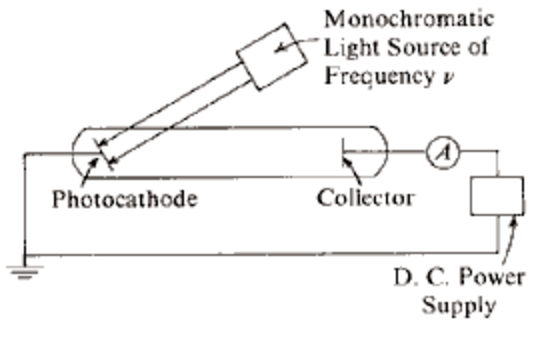
\includegraphics[width=\linewidth, height=50mm]{images/PhotoEE.png}
      \tiny (GRE 8677 \#31-33)
    \end{minipage}

\\ \hline

Photoelectric effect & Light is absorbed in quanta:  $E = h \nu$ \\
& \begin{minipage}{.4\textwidth}
 $|eV_0|= K_{max} = h \nu - W $ where $V_0$ is the stopping potential ($I=0$), $K_{max}$ is the maximum kinetic energy of an emitted electron, and $W$ is the work function of the metal. $W = h \nu_0$, where $\nu_0$ is the threshold frequency.
    \end{minipage}

\\ \hline
}

\Table{
\hline

Compton effect & 
\begin{minipage}{.3\textwidth}
      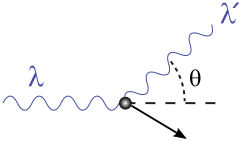
\includegraphics[width=\linewidth, height=25mm]{images/ComptonScat.png}
      \end{minipage}
      \\
      &
      \begin{minipage}{.6\textwidth}
       ``inelastic scattering of a photon by a charged particle, usually an electron. It results in a decrease in energy (increase in wavelength) of the photon (which may be an X ray or gamma ray photon)''
    \tiny \url{https://en.wikipedia.org/wiki/Compton_scattering}
    \end{minipage}
    \\
    &
    $\lambda' - \lambda = \dfrac{h}{m_e c} (1- \cos \theta)$
\\ \hline
}

\Table{
\hline

Franck-Hertz experiment & 
\begin{minipage}{.6\textwidth}
      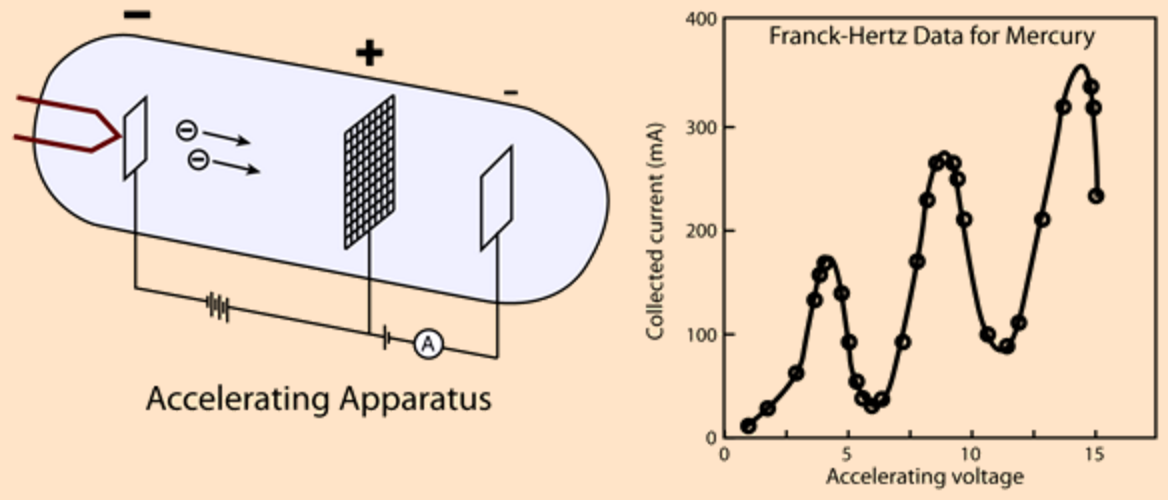
\includegraphics[width=\linewidth, height=45mm]{images/FranckHertz.png}
      \end{minipage}
      \\
      &
      \begin{minipage}{.6\textwidth}
       ``Electrons were accelerated by a voltage toward a positively charged grid in a glass envelope filled with \textbf{mercury vapor}. Past the grid was a collection plate held at a small negative voltage with respect to the grid. The values of accelerating voltage where the current dropped gave a measure of the energy necessary to force an electron to an excited state.'' \tiny \url{http://hyperphysics.phy-astr.gsu.edu/hbase/frhz.html}
    
    \end{minipage}
    
    
    
    
\\ \hline
}

\Table{
\hline

Angular momentum values & 
\MiniPg{.6}{
$l = 0,1,2,3,4,5,6,7,8$

$l = s,p,d,f,g,h,i,k,l$ 

For a given $n$, $l$ can take values up to $n-1$.

 Archaic: `s'harp, `p'rincipal, `d'iffuse, `f'undamental
}
\\ \hline
}

%%%%%%%%%%%%%%%%%%%%%%%%%%%%%%%%%%%%%%%%%

\subsection{Atomic structure} 
\Table{
\hline

State of an electron
&
\MiniPg{.7}{
\center

 $\psi(\bold{r}) \chi({\bold{s})}$
 \flushleft
 
Where $\psi$ is the spatial wave function and $\chi$ is the spinor.

Recall the composite spin states. The singlet state is antisymmetric and hence must be joined with a symmetric spatial function. Each triplet state is symmetric and requires a antisymmetric spatial function.

}

\\ \hline

Aufbau principle
&
\MiniPg{.7}{
      ``Hypothetically, electrons orbiting one or more atoms fill the lowest available energy levels before filling higher levels.''

\GraphicWHN{.6}{.5}{aufbau.png}

      \tiny \url{http://study.com/cimages/multimages/16/aufbau.png}
}

\\ \hline

Diagonal rule

&

\MiniPg{.7}{
\center
Orbitals are filled in order of increasing $n+l$ value.  $nl$:

\GraphicWHN{.25}{.2}{DiagonalOrdering.png}

\tiny \url{https://en.wikipedia.org/wiki/Aufbau_principle}

}

\\ \hline
}

%%%%%%

\Table{
\hline

\MiniPg{.3}{
Total angular momentum
}

&

$j = l + s$

\\ \hline

Hund's Rules

&

\begin{minipage}{.7\textwidth}
      I) Consistent with Pauli exclusion, the state with the highest total spin ($S$) has the lowest energy: $\uparrow S \equiv \downarrow E$
      
      II) For a given spin, the state with the highest total orbital angular momentum ($L$), consistent with overall antisymmetrization, will have the lowest energy. $\uparrow L \equiv \downarrow E$
      
      III) If a subshell ($n,l$) is no more than half-filled, then the lowest energy level has $J=|L-S|$; if it is more than half-filled, then $J = L + S$ has the lowest energy.
\end{minipage}

\\ \hline

Hieroglyphic & $^{2S+1}L_J$

\\ \hline
}

\Table{
\hline

First 36 configs. & \begin{minipage}{.3\textwidth}
      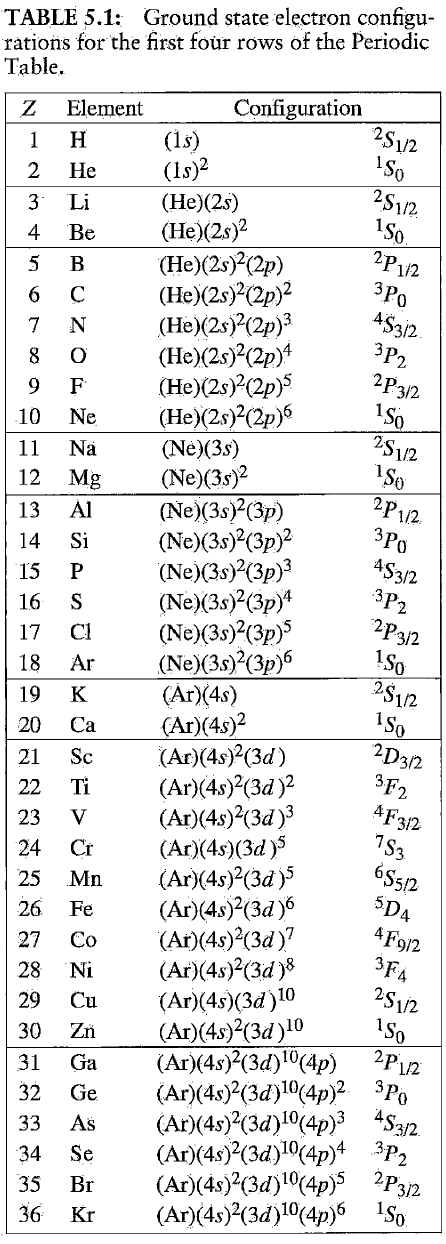
\includegraphics[width=\linewidth, height=125mm]{images/36Configs.png}
      \tiny Giffiths, \textit{Quantum}
    \end{minipage}

\\ \hline
}


%%%%%%%%%%%%%%%%%%%%%%%


\subsection{Atomic Spectra} 

\subsection{Selection rules}
\center
\begin{tabular}{|c|c|}
\hline

Selection rule for $m$ & No transitions occur unless $\Delta m = \pm1 \textrm{ or } 0$.

\\ \hline

Selection rule for $l$ & No transitions occur unless $\Delta l = \pm1$.
\\
&
\begin{minipage}{.6\textwidth}
      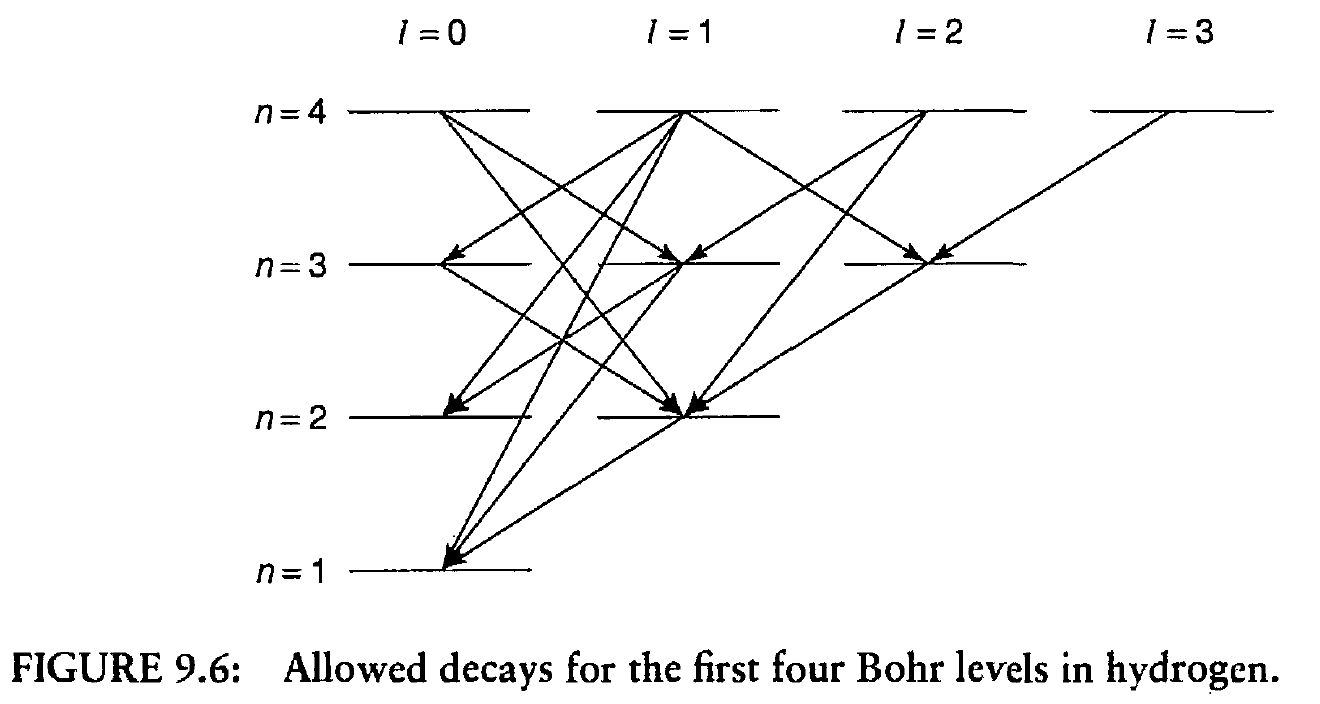
\includegraphics[width=\linewidth, height=50mm]{images/SelectionRuleL.png}
      \tiny Griffiths, \textit{Quantum Mechanics}
    \end{minipage}

\\ \hline
\end{tabular}
\flushleft

%%%%%%%%%%%%%%%%%%%%%%%%%%%%%%%%%%%%%%

\subsection{X-rays} 
\center

\begin{figure}[htbp]
    \begin{center}
	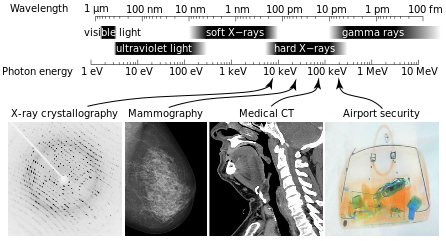
\includegraphics[width=110mm]{images/Xrays.png}
    \end{center}
    \linespread{1} 
	\caption[X-rays]{
	\tiny https://en.wikipedia.org/wiki/X-ray
	}
\label{xrays}
\end{figure}


%%%%

\begin{tabular}{|c|c|}
\hline

Xray transitions & \begin{minipage}{.5\textwidth}
      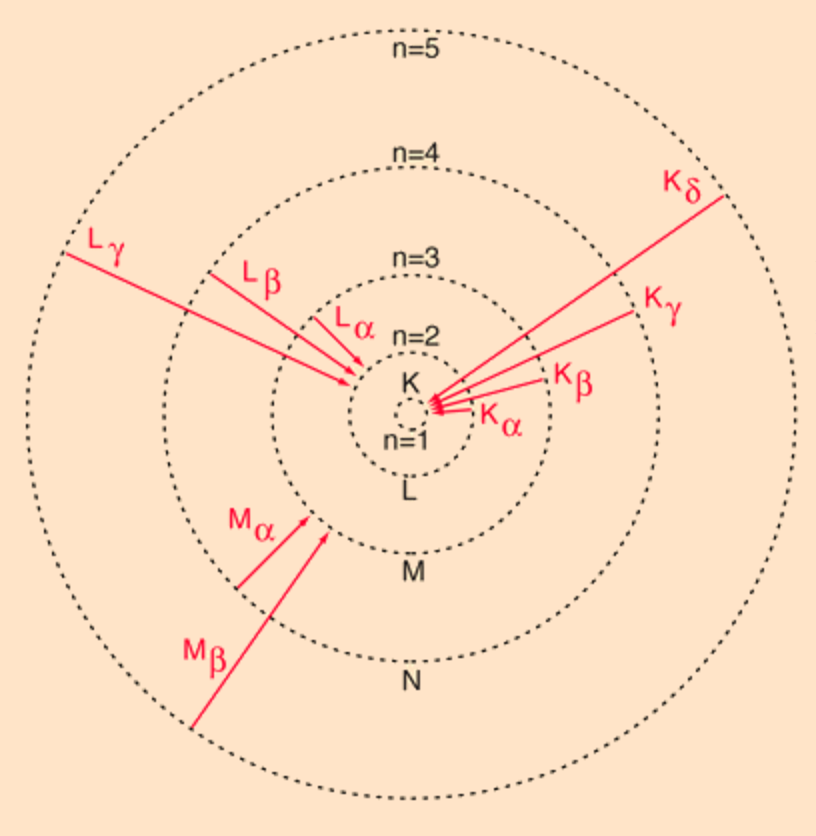
\includegraphics[width=\linewidth, height=80mm]{images/XrayTransitions.png}
      \tiny \url{http://hyperphysics.phy-astr.gsu.edu/hbase/quantum/xterm.html}
    \end{minipage}

\\ \hline

Moseley's Law & \\
\& description & 

\\ \hline
\end{tabular}
\flushleft

%%%%%%%%%%%%%%%%%%%%%%%%%%%%%%%%%%%%%%

\subsection{Atoms in electric and magnetic fields} 



\section{Nuclear and Particle}
nuclear properties, radioactive decay, fission
and fusion, reactions, fundamental
properties of elementary particles



\subsection{Light and matter interaction} 
\center
\begin{tabular}{|c|c|}
\hline

Scattering Cross Section & \begin{minipage}{.7 \textwidth}
\small

$\sigma = \dfrac{\mu}{n} = \dfrac{1}{n\Phi}\Big(- \dfrac{d\Phi}{dz}\Big) = \dfrac{1}{nIA}\dfrac{dW}{dz} = \dfrac{P}{\rho l}$, where 

$\sigma$ is the cross section of the event (m$^2$);  

$\mu$ is the attenuation coefficient due to the occurrence of this event (m$^{-1}$); $n$ is the number density of the target particles (m$^{-3}$);

$\Phi$ is the flux of the incident beam;

$-d\Phi$ is the amount of flux lost due to the occurrence of the event (i.e. amount scattered);

$dz$ is the thickness of the target material;

$I$ is the particle flux(or intensity) of the incident beam (m$^{-2}$s$^{-1}$);

$A$ is the area of overlap between beam and target (m$^2$);

$dW$ is the rate at which the event occurs (s$^{-1}$);

$P$ is the probability that a beam particle is scattered;

$\rho$ is the number density ($N/V$) of target particles;

$l$ is the length of the sample (i.e. same as $dz$).

\textbf{If a scattering question is asked, you can probably use dimensional analysis assuming linear relations.}
\end{minipage}

\\ \hline
\end{tabular}


\begin{tabular}{|c|c|}
\hline
\begin{minipage}{.3\textwidth}
Energy ranking of the four major light/matter interactions
\end{minipage}

&
\begin{minipage}{.6\textwidth}

(low energy) Photoelectric $\rightarrow$ Thomson $\rightarrow$ Compton $\rightarrow$ Pair production (high energy)
\end{minipage}

\\ \hline
\end{tabular}
\flushleft

%%%%%%%%%%%%%%%%%%%%%%%%%%%%%%%%%%%%%%%%

\subsection{Particles}

\MiniPg{1}{

\GraphicWHN{.8}{.6}{whatparticle.png}
\tiny .
}

\Table{
\hline

Bosons, Hadrons, Fermions

&

\begin{minipage}{.5\textwidth}
      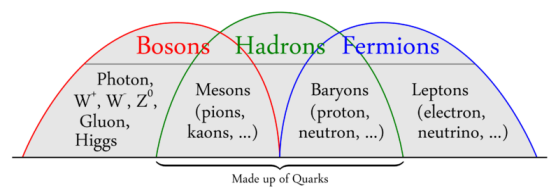
\includegraphics[width=\linewidth, height=30mm]{images/Bosons-Hadrons-Fermions.png}
       \tiny \url{https://commons.wikimedia.org/wiki/File:Bosons-Hadrons-Fermions-RGB-png2.png}

    \end{minipage}

\\ \hline
}

%%%%

\Table{
\hline

The Standard Model & \begin{minipage}{.5\textwidth}
      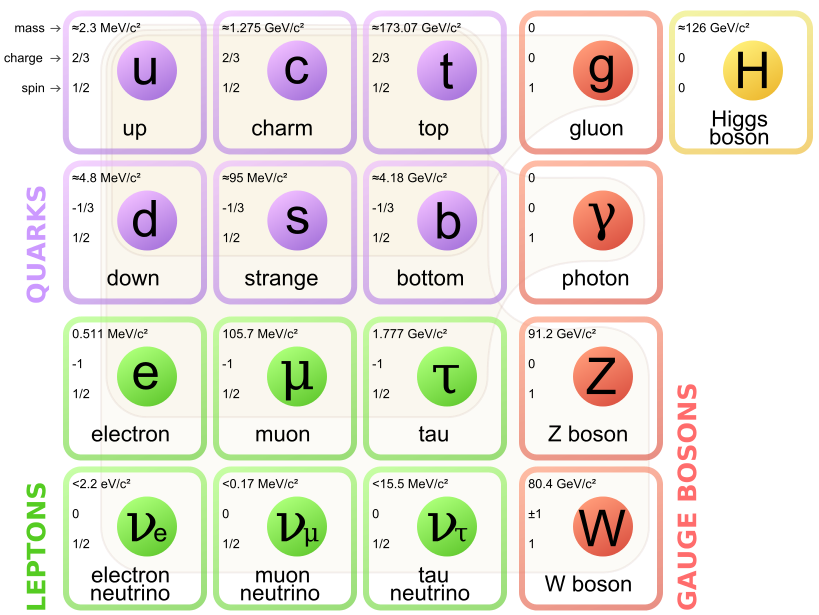
\includegraphics[width=\linewidth, height=60mm]{images/StdMod.png}
       \tiny \url{https://en.wikipedia.org/wiki/Standard_Model}

    \end{minipage}
\\ \hline
}

%%%%

\Table{
\hline

Protium & $^1H$

\\ \hline

Deuterium & 
\begin{minipage}{0.6 \textwidth}

Symbol: D or $^2$H. Also known as `heavy hydrogen'. Nucleus consists of one proton and one neutron.

\end{minipage}

\\ \hline
}

%%%%

\Table{
\hline

Deuteron & 
\begin{minipage}{0.6 \textwidth}
The nucleus of deuterium. It is a boson and exists in the triplet state. The singlet state is virtual and only transiently exists during neutron-proton inelastic scattering. Duh!

\end{minipage}

\\ \hline
}

%%%%

\Table{
\hline

Tritium &
\begin{minipage}{0.6 \textwidth}

T or $^3$H. One proton, two neutrons. Watch out.

\end{minipage}

\\ \hline

Triton & Yup. You guessed it.

\\ \hline
}

%%%%%%%%%%%%%%%%%%%%%%%%%%%%%%%%%%

\subsection{Nuclear properties}
\Table{
\hline

\MiniPg{.25}{
Nuclear binding energy
}
&
\begin{minipage}{.75\textwidth}
      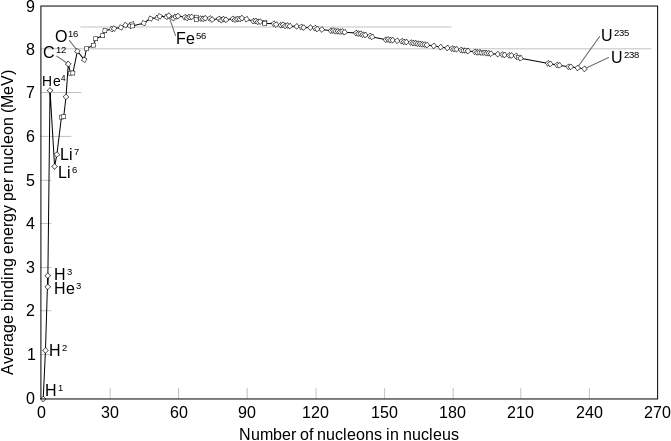
\includegraphics[width=\linewidth, height=60mm]{images/NucBindingEn.png}
      
      \small
      
    \textbf{H to Na} -  increasing ``forces per nucleon in the nucleus, as each additional nucleon is attracted by other nearby nucleons, and thus more tightly bound to the whole.";
   \textbf{Mg to Xe} (``saturation") - ``the nucleus has become large enough that nuclear forces no longer completely extend efficiently across its width. Attractive nuclear forces in this region, as atomic mass increases, are nearly balanced by repellent electromagnetic forces between protons, as the atomic number increases.";
   \textbf{Cs to U} - ``electromagnetic repulsive forces are beginning to overcome the strong nuclear force attraction."
   
   \tiny \url{https://en.wikipedia.org/wiki/Nuclear_binding_energy}
    \end{minipage}
 
 \\ \hline
}

%%%%%%%%%%%%%%%%%%%%%%%%%%%%%%%%%%%%%%%
\subsection{Radioactive decay} 
\Table{
\hline
\MiniPg{.3}{
Alpha decay, beta decay, gamma decay, positron emission, electron capture
}

&

\MiniPg{.7}{

\GraphicWHN{1}{.7}{RadioDecay.png}

\tiny \url{http://chemwiki.ucdavis.edu/Textbook_Maps/General_Chemistry_Textbook_Maps/Map\%3A_Chemistry_(OpenSTAX)/21\%3A_Nuclear_Chemistry/21.3\%3A_Radioactive_Decay}

}

\\ \hline
}
%%%%%%%%%%%%%%%%%%%%%%%%%%%%%%%%%%%%%%%

\subsection{Fission and fusion} 
\Table{
\hline
Deuterium tritium fusion

&

\MiniPg{.6}{
\GraphicWHN{.5}{.5}{DeutTritFusion.png}
\tiny \url{https://en.wikipedia.org/wiki/Nuclear_fusion}
}
 
 \\ \hline
}

%%%%
\Table{
\hline

Deuterium Deuterium fusion

 &
 
\MiniPg{.6}{
\GraphicWHN{.9}{.6}{DeutDeutFusion.jpg}
\tiny \url{http://resource.download.wjec.co.uk/vtc/2008-09/science/irf08_48/Images/Nuclear-fusion.jpg}

}
 
 \\ \hline
}

%%%%

\Table{
\hline
\MiniPg{.4}{\center
Proton Proton chain fusion reaction in the sun and smaller stars
}

&

\MiniPg{.6}{\center

\GraphicWHN{.4}{.6}{FusionintheSun.png}
\tiny \url{https://en.wikipedia.org/wiki/Nuclear_fusion}
}

\\ \hline
}

%%%%%%%%%%%%%%%%%%%%%%%%%%%%

\subsection{Reactions} 
\center
\begin{tabular}{|c|c|}
\hline

Chemical symbol convention & $^{A}_{Z}Na^{C} $ \\
& where $A = $ Mass \# of protons $+$ neutrons, \\
& $Z =$ Atomic \# of protons, \\
& $C = $ Charge, e.g. '$+2$'
 
 \\ \hline
\end{tabular}
\flushleft

%%%%%%%%%%%%%%%%%%%%%%%%%%%%%%%%%%%%%%%%

\subsection{Fundamental properties of elementary particles} 





\section{Special Relativity}
(such as introductory concepts, time dilation,
length contraction, simultaneity,
energy and momentum, four-vectors
and Lorentz transformation,
velocity addition)

\subsection{Introductory concepts} 
\center
\begin{tabular}{|c|c|}
\hline

 An \textit{event} is ... & ... a location and a time: $(x, y, z, c t).$

\\ \hline

$\beta =$ & $v/c$ generally $<1$

\\ \hline

$\gamma = $ & $\dfrac{1}{\sqrt{1 - \beta^2}}$ generally $>1$

\\ \hline
\end{tabular}
\flushleft

%%%%

\subsection{Lorentz invariant intervals}
\center
\begin{tabular}{|c|c|}
\hline

Lorentz invariant interval & $ s^2 = \Delta x^2 + \Delta y^2 + \Delta z^2 - (c \Delta t)^2 $\\
& $ = \Delta x'^2 + \Delta y'^2 + \Delta z'^2 - (c \Delta t')^2$

\\ \hline

Time-like interval,  & Enough time passes between two events that \\ 
description and inequality:  &they could be causally related. \\
& $s^2 < 0$ or $c^2 \Delta t^2 > \Delta r^2$

\\ \hline

Proper time interval & Would be measured by an observer traveling\\
$\Delta \tau $ & between two time-like events in an inertial frame.  \\
 & $ \Delta \tau = \sqrt{\Delta t^2 - \dfrac{ \Delta r^2}{c^2}} $

\\ \hline

Light-like interval & Events which which occur to or are \\
 & initiated by a photon along its path. \\
 & $s^2 = 0 $ or $c^2 \Delta t^2 = \Delta r^2$

\\ \hline

\end{tabular}

\begin{tabular}{|c|c|}
\hline

Space-like interval & Not enough time between the events for \\
 & the possibility of a causal relation. There exists a \\
  & ref. frame in which the two events are simultaneous, \\ 
   & but no ref. frame in which they occur in the spatial location. \\ 
   & $s^2 > 0$ or $c^2 \Delta t^2 < \Delta r^2$
   
\\ \hline

Proper distance & The measurement of space-like separation between events. \\
 $\Delta \sigma $ & $\Delta \sigma = \sqrt{s^2} = \sqrt{\Delta r^2 - c^2 t^2} $

\\ \hline
\end{tabular}
\flushleft



\subsection{Time dilation} 
\center
\begin{tabular}{|c|c|}
\hline

`Moving clocks run ... & ... slower.'

\\ \hline

Proper time & Time read on the face of the moving clock (i.e. clock's ref. fr.) \\
$\Delta \tau = $ & $\dfrac{\Delta t}{\gamma}$ \\ 
 & Lorentz invariant
 
\\ \hline
\end{tabular}
\flushleft

%%%%

\Table{
\hline

Relativistic Doppler Effect

&

\MiniPg{.6}{\center
$\dfrac{\lambda_o}{\lambda_s} = \sqrt{\dfrac{1 + \beta}{1 - \beta}}$

$\beta = \dfrac{ (\frac{\lambda_o}{\lambda_s})^2 - 1}{(\frac{\lambda_o}{\lambda_s})^2 + 1}$

Where $\beta$ is $v/c$ and $+v$ means the object is going away from the observer.
}

\\ \hline
}

%%%%%%%%%%%%%%%%%%%%%%%%%%%%%%%%%%%%

\subsection{Length contraction} 
\center
\begin{tabular}{|c|c|}
\hline

`Moving sticks are...  & ... shorter.'

\\ \hline

Proper length & Length measured in ref. fr. of the stick. \\
$\Delta L_0$ & $\Delta L_0 = \gamma \Delta L$
 
 \\ \hline
\end{tabular}
\flushleft

%%%%%%%%%%%%%%%%%%%%%%%%%%

\subsection{Simultaneity}

%%%%%%%%%%%%%%%%%%%%%%%%%%

\subsection{Energy and momentum} 
\Table{
\hline

\MiniPg{.4}{
\center

For a particle with rest mass $m_0$ and velocity $\vec v$

$\bold{p} = $

}

& 

$\gamma m_0 \bold{v}$

\\ \hline

$E = $ & $\gamma m_0 c^2 = RestE + KE$

\\ \hline

Kinetic energy & $KE = E - RestE = mc^2 - m_0 c^2 = m_0 c^2 (\gamma - 1)$

\\ \hline

Energy and momentum relation

& 

\MiniPg{.6}{
\center
\MPalign{
p^2 c^2 & = \gamma^2 m_0^2 v^2 c^2 \\
		& = \gamma^2 m_0^2 \dfrac{v^2}{c^2} c^4 \\
		& = \gamma^2 \BigP{ m_0^2 \dfrac{v^2}{c^2} c^4 - m_0^2 c^4 + m_0^2 c^4} \\
		& = \gamma^2 \BigP{ m_0^2 c^4 \BigP{ \dfrac{v^2}{c^2} - 1 } + m_0^2c^4} \\
		& = -m_0^2c^4 + \gamma^2 m_0^2 c^4
 }
 
Rearrange: $\boxed{E^2 = (pc)^2 + (m_0 c^2)^2}$

} 
 \\ \hline
}

%%%%%%%%%%%%%%%%%%%%%%%%%%%%%%%%

\subsection{Lorentz transformation} 
\center
\begin{tabular}{|c|c|}
\hline
Lorentz transformation & \\

$x' = $ & $\gamma(x - \beta ct)$ \\

$ct' = $ & $ \gamma(ct - \beta x)$

\\ \hline

Inverse Lorentz Transformation & $v \rightarrow -v$ \\

$x = $ & $\gamma(x'+ \beta ct') $ \\

$ct = $ & $\gamma (ct' + \beta x')$

\\ \hline

Electromagnetic fields & $\bold{E'}_{\parallel} = \bold{E}_{\parallel}$ \\
parallel and perpendicular to $\bold{v}$ & $\bold{B'}_{\parallel} = \bold{B}_{\parallel}$ \\
& $\bold{E'_{\bot}} = \gamma (\bold{E}_{\bot} + \bold{v} \times \bold{B})$ \\
& $\bold{B'}_{\bot} = \gamma\Big(\bold{B}_{\bot} - \dfrac{1}{c^2}\bold{v}\times\bold{E}\Big)$

\\ \hline
\end{tabular}
\flushleft

\subsection{Derivation of $E=mc^2$ using four-vectors} 
\center
\begin{tabular}{|c|c|}
\hline

$x^\mu =  $& $(x,y,z,ct) $ where $\mu = 1,2,3,4$

\\ \hline

$x_\mu = $ & $(x,y,z,-ct)$

\\ \hline

$x^\mu x_\mu = $ & $(x^2+y^2+z^2-(ct)^2$

\\ \hline

$\Delta x^\mu =$ & $(\Delta x, \Delta y, \Delta z, c \Delta t) = ( \Delta \vec r, c \Delta t)$

\\ \hline

$\dfrac{\Delta x^\mu}{\Delta \tau} = $ & $\gamma \dfrac{\Delta x^\mu}{\Delta t} $\\

 & $ = (\gamma v_x, \gamma v_y, \gamma v_z, \gamma c) $ \\

four-velocity & $ = (\gamma \vec v, \gamma c) $

\\ \hline

$m \dfrac{\Delta x^\mu}{\Delta \tau} = $ &  $m \gamma \dfrac{\Delta x^\mu}{\Delta t} $\\

four-momentum & $=  (\gamma m \vec v, \gamma m c) = p^\mu$

\\ \hline

$p^\mu p_\mu = $ & rest frame,  $\gamma = 1$, so $p^\mu = (0, mc)$ \\

rest and non-rest frames & non-rest, $p^\mu = (\gamma m \vec v, \gamma m c) $ \\

 &  four-vector dot product is invariant, \\ 
 & so $p^\mu p_\mu$ is the same for rest and non-rest: \\
& $p^\mu p_\mu = (\gamma m v)^2 - (\gamma m c)^2 = -(mc)^2$

\\ \hline

\end{tabular}

\begin{tabular}{|c|c|}
\hline

 $(\gamma m v)^2 - (\gamma m c)^2 = -(mc)^2$& $(p)^2 - (E/c)^2 = -(mc)^2$ \\
 Rewrite, solve in terms of $E$. & Multiply by $c^2$ and rearrange. \\ 
 & $E^2 = (pc)^2 + (mc^2)^2$

\\ \hline
\end{tabular}
\flushleft


\subsection{Four-vectors and Lorentz transformation} 


\subsection{Relativistic Velocity Addition} 
\center
\begin{tabular}{|c|c|}
\hline

$v_{tot} = $ & $ \dfrac{v_1 + v_2}{1 + \dfrac{v_1 v_2}{c^2}} $

 \\ \hline
\end{tabular}
\flushleft


\subsection{Twin astronauts problem} 






\section{Laboratory Methods}
(such as data and error analysis, electronics,
instrumentation, radiation detection,
counting statistics, interaction of
charged particles with matter, lasers
and optical interferometers, dimensional
analysis, fundamental applications
of probability and statistics)

%%%%%%%%%%%%%%%%%%%%%%%%%%%%%%%%%%%%%%%

\subsection{Data and error analysis} 
\Table{
\hline

Semi-log (lin-log and log-lin) & \begin{minipage}{.375\textwidth}
      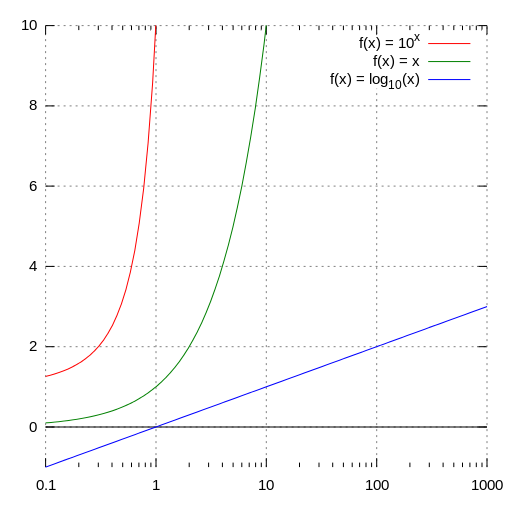
\includegraphics[width=\linewidth, height=60mm]{images/LinLog.png}
    \end{minipage} \\
    
Plot 3 characteristic $f(x)$ & \begin{minipage}{.375\textwidth}
      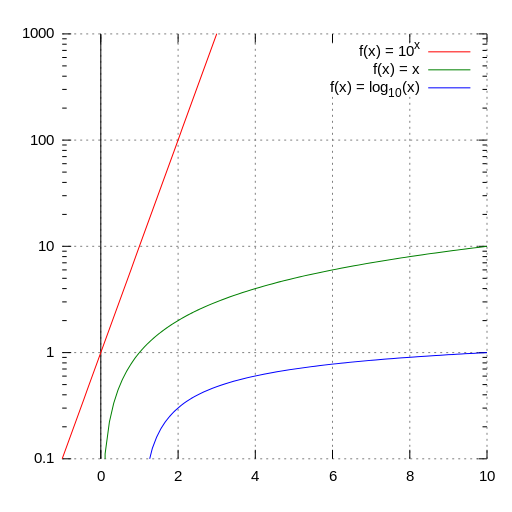
\includegraphics[width=\linewidth, height=60mm]{images/LogLin.png}
      \tiny \url{https://en.wikipedia.org/wiki/Semi-log_plot}
    \end{minipage} 

\\ \hline

Plot 3 characteristic $f(x)$ for log-log &\begin{minipage}{.375\textwidth}
      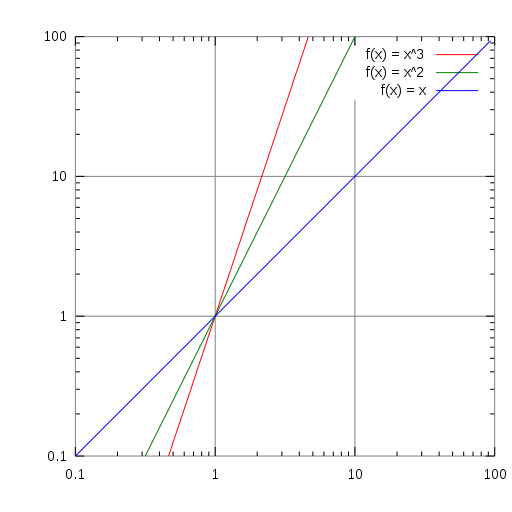
\includegraphics[width=\linewidth, height=60mm]{images/LogLog.png}
      \tiny \url{https://en.wikipedia.org/wiki/Log\%E2\%80\%93log_plot}
    \end{minipage} 
 
  \\ \hline
}


\Table{
\hline

\MiniPg{.5}{
Uncertainty or error $\delta R$ for $R(X,Y,...)$
}

&

\MiniPg{.5}{\center
$\delta R = \sqrt{ \Big(\dfrac{\partial R}{\partial X} \cdot \delta X \Big)^2 + \Big( \dfrac{\partial R}{\partial Y } \cdot \delta Y \Big)^2 + ... }$
}

\\ \hline
\MiniPg{.5}{
Addition of measured quantities
}

&

\MiniPg{.5}{
\center
$R = X + Y -Z$


$\delta R \approx \delta X + \delta Y + \delta Z$

$\delta R = \sqrt{(\delta X)^2 + (\delta Y)^2 + (\delta Z)^2} $

}

\\ \hline
\MiniPg{.5}{
Multiplication of measured quantities
}

&

\MiniPg{.5}{
\center
$R = \dfrac{X \cdot Y}{ Z}$


$\dfrac{\delta R}{|R|} \approx \dfrac{\delta X}{|X|} + \dfrac{\delta Y}{|Y|} + \dfrac{\delta Z}{|Z|}$

$\delta R = |R| \cdot \sqrt{\Big(\dfrac{\delta X}{|X|}\Big)^2 + \Big(\dfrac{\delta Y}{|Y|}\Big)^2 +\Big (\dfrac{\delta Z}{|Z|}\Big)^2} $

}

\\ \hline
\MiniPg{.5}{
Multiplication of with a constant
}

&

\MiniPg{.5}{
\center
$R = c \cdot X$

$\delta R = |c| \cdot \delta X $

}

\\ \hline
\MiniPg{.5}{
Polynomial functions
}

&

\MiniPg{.5}{
\center
$R = X^n$

$\delta R = |R| \cdot |n| \cdot \dfrac{\delta X}{|X|}  $

\tiny \url{http://lectureonline.cl.msu.edu/~mmp/labs/error/e2.htm}

}

\\ \hline
}


%%%%%%%%%%%%%%%%%%%%%%%%%%%%%%%%%%%%%%%

\subsection{Electronics} 

%%%%%%%%%%%%%%%%%%%%%%%%%%%%%%%%%

\subsection{Instrumentation} 

%%%%%%%%%%%%%%%%%%%%%%%%%%%%%%%%%

\subsection{Radiation detection} 

%%%%%%%%%%%%%%%%%%%%%%%%%%%%%%%%%

\subsection{Counting statistics} 
\center
\begin{tabular}{|c|c|}
\hline

Poisson distribution &  $P(k \textrm{ events in interval}) = \dfrac{\lambda^ke^{-k}}{k!}$ \\
\hline
When to use? & $\lambda$ is the avg. \# of events per interval. \\
& $k$ is the integer \# of times an event occurs in an interval. \\
& Events occur independently. \\
& Constant rate of occurrence. \\
& Events cannot be identical in space and time. \\
& Probability of an event in an interval $\propto$ length of interval. \\
& e.g. \# of decays from a radioactive sample over 1 hour. \\
\hline
Properties & mean = variance = $\lambda$, so $\sigma = \sqrt{\textrm{var}} = \sqrt{\lambda}$ \\
& If $\lambda > $ about 10, normal distribution is good approximation \\
& if continuity correction is used. See:\\
& \url{https://en.wikipedia.org/wiki/Poisson_distribution}

 \\ \hline
\end{tabular}
\flushleft

\subsection{Interaction of charged particles with matter} 

%%%%%%%%%%%%%%%%%%%%%%%%%%%%%%%%%

\subsection{Lasers and optical interferometers} 

\Table{
\hline

Laser

&

\MiniPg{.7}{
\center
Light amplification by stimulated emission of radiation

\GraphicWHN{.75}{.5}{laser.jpg}
\tiny \url{http://micro.magnet.fsu.edu/primer/java/lasers/stimulatedemission/}

}

\\ \hline
}

%%%%

\Table{
\hline

Stimulated emission

&
\MiniPg{.7}{
\GraphicWHN{.8}{.4}{stimulatedEmission.png}
\tiny \url{https://en.wikipedia.org/wiki/Laser}
}
\\ \hline
}


%%%%%%%%%%%%%%%%%%%%%%%%%%%%%%%%%

\subsection{Dimensional analysis} 

%%%%%%%%%%%%%%%%%%%%%%%%%%%%%%%%%

\subsection{Fundamental applications of probability and statistics}  





\section{Miscellany}
Condensed Matter (e.g., crystal
structure, x-ray diffraction, thermal
properties, electron theory of metals,
semiconductors, superconductors)
Miscellaneous (e.g., astrophysics, mathematical
methods, computer applications)

\subsection{Chemistry}

%%%%%%%%%%%%%%%%%%%%%%%%%%%%%%%%%

\subsection{Plasma}
\Table{
\hline

Debye length & $\lambda_D = \sqrt{ \dfrac{\epsilon_0 k_B T_e}{n_eq_e^2}} $

\\ \hline
}

\subsection{Condensed Matter} 

%%%%%%%%%%%%%%%%%%%%%%%%%%%%%%%%%

\subsection{Crystal structure} 

%%%%%%%%%%%%%%%%%%%%%%%%%%%%%%%%%

\subsection{X-ray diffraction} 
\center
\begin{tabular}{|c|c|}
\hline

Bragg Diffraction &

\begin{minipage}{0.6\textwidth}

 $n \lambda = 2d \sin \theta$ like a thin film, but using a different angle, i.e. the angle between the beam and the surface plane.
 
 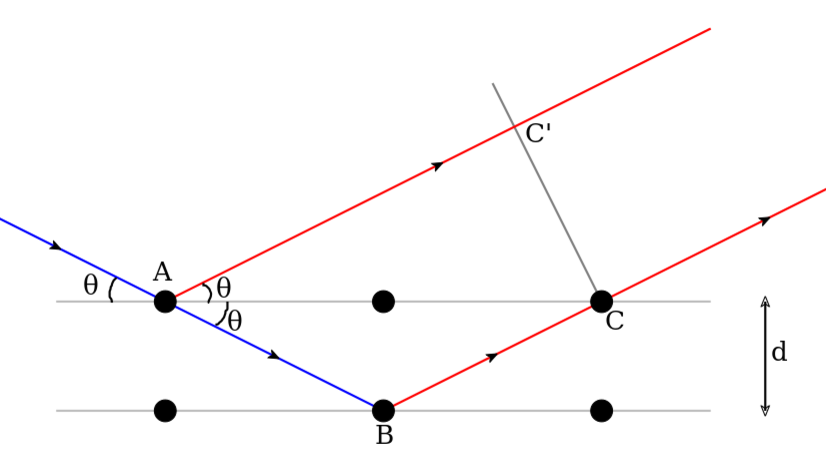
\includegraphics[width=75mm, height=50mm]{images/Bragg.png}
      \tiny \url{https://en.wikipedia.org/wiki/Bragg\%27s_law}
\end{minipage}

\\ \hline
\end{tabular}
\flushleft

\subsection{Thermal properties} 

%%%%%%%%%%%%%%%%%%%%%%%%%%%%%%%

\subsection{Electron theory of metals}
\center
\begin{tabular}{|c|c|}
\hline

\MiniPg{.4}{

At the highest energies of the valence band in many semiconductors (Ge, Si, GaAs, ...), and the lowest energies of the conduction band in some semiconductors (GaAs, ...), the band structure $E(\bold{k})$ can be locally approximated as

}

&
 
$E(\bold{k}) = E_0 + \dfrac{\hbar^2 \bold{k}^2}{2m^*}$
 
\\ \hline

\MiniPg{.4}{

Effective mass of electron in metals

}
 
& 

\MiniPg{.6}{
\center

\MPalign{
E & = \dfrac{\hbar^2 k^2}{2m} \\
\dfrac{dE}{dk} & = \dfrac{\hbar^2 k}{m} = \hbar v_g \\
\dfrac{dv_g}{dt} &= \dfrac{1}{\hbar} \dfrac{d^2E}{dt^2} \dfrac{dk}{dt} = \dfrac{1}{\hbar} \dfrac{d^2E}{dt^2} \dfrac{F}{\hbar} \\
F &= \hbar^2 \BigP{\dfrac{d^2E}{dt^2}}^{-1} \dfrac{dv_g}{dt} \\
m^* &= \hbar^2 \BigP{\dfrac{d^2E}{dt^2}}^{-1} 

}

}

\\ \hline
\end{tabular}
\flushleft

%%%%%%%%%%%%%%%%%%%%%%%%%%%%%%%%%


\subsection{Semiconductors}
\Table{
\hline

\MiniPg{.3}{\center
$n$-doped semiconductor
}

&

\MiniPg{.7}{\center
$n$ stands for negative, so $n$-type silicon is doped with negatively charged atoms (say, phosphorus) . This means that these atoms have extra electrons, and can easily part with the extra electron. Hence, they are donors.
}

\\ \hline
}

%%%%

\Table{
\hline

\MiniPg{.3}{\center
$p$-doped semiconductor
}

&

\MiniPg{.7}{\center
$p$ stands for positive, so $p$-type silicon is doped with positively charged atoms (say, boron). This means that these atoms have missing electrons, so they can easily accept new electrons to fill the vacancy. Hence, they are acceptors.
}

\\ \hline
}

%%%%%%%%%%%%%%%%%%%%%%%%%%%%%%%%%

\subsection{Superconductors} 

%%%%%%%%%%%%%%%%%%%%%%%%%%%%%%%%%

\subsection{Astrophysics} 

\Table{
\hline

Schwarzschild radius

&

$R = \dfrac{2MG}{c^2}$

\\ \hline
}

%%%%%%%%%%%%%%%%%%%%%%%%%%%%%%%%%

\subsection{Mathematical methods}

%%%%%%%%%%%%%%%%%%%%%%%%%%%%%%%%%

\subsection{Computer applications}





\end{document}

%%%%%%%%%%%%%%%%%%%%%%%%%%%%%%%%%
%===========================================%
%%%%%%%%%%%%%%%%%%%%%%%%%%%%%%%%%